\documentclass [a4paper, 12pt]{book}
\usepackage [italian] {babel}	
\usepackage{graphicx}
\usepackage{hyperref}
\usepackage{listings}
\usepackage{color}
\graphicspath{ {../Screenshots/} }



\definecolor {background}{RGB}{237,241,247}
\definecolor{commentColor}{rgb}{0.4,0.4,0.4}
\definecolor {keywordColor}{RGB}{224,162,4}
\definecolor {stringColor}{RGB}{142,74,49}
\definecolor{tagColor}{rgb}{0.0,0.0,0.6}

\lstdefinestyle{XML}{
	language = XML,
	extendedchars=true,
	breaklines = true,
	breakatwhitespace=true,	
	basicstyle=\ttfamily\footnotesize,
	columns=fullflexible,
	commentstyle=\color{commentColor}\upshape,
	morecomment=[s]{<?}{?>},
	backgroundcolor = \color{background},
	keywordstyle = \color{keywordColor},
	stringstyle = \ttfamily\color{black}\normalfont,
	tagstyle = \color{tagColor}\bf,
	showstringspaces=false,
	otherkeywords ={codFisc=,numero=,id=,tipologia=,xmlns:xsi=,
	xsi:noNamespaceSchemaLocation=,xmlns:xsd=,name=,ref=,minOccurs=,maxOccurs=,
	type=,use=,base=,value=},
}



\begin{document}
\author{Angelo Trifelli , Simone Amoriello}
\title{Tesina LWEB}
\maketitle
\tableofcontents

\chapter{Introduzione e descrizione dei dati}

Si propone di realizzare un sito web dedicato ad un hotel ed in grado di permettere all'utente di usufruire di tutte le varie funzionalità che l'hotel mette a disposizione.\\\\
Il sito è visitabile a partire da una pagina home iniziale, accessibile da tutte le tipologie di utenti, che descrive l'hotel fornendo informazioni su quest'ultimo, una serie di FAQ ed alcune attività che vengono messe a disposizione. Dalla home è poi possibile accedere ad una pagina dedicata per la prenotazione di una camera oppure direttamente alla schermata di login nel caso in cui l'utente è già cliente dell'hotel.\\\\
Il login (mediante username e password) può essere effettuato da tre tipologie di utenti:
\begin{itemize}
\item \textbf{Utente registrato:} cioè un utente che deve essere necessariamente registrato all'interno del sito dell'hotel. La registrazione può essere effettuata dall'utente in un qualunque momento e solo dopo averla effettuata l'utente potrà prenotare una camera.
\item \textbf{Concierge:} utente moderatore che disporrà di credenziali personali e potrà svolgere operazioni volte alla moderazione del sito.
\item \textbf{Admin:} un utente amministratore che disporrà di credenziali personali e che potrà effettuare operazioni riservate.
\end{itemize}
Nel caso in cui il login venga effettuato da un utente registrato allora si verrà portati in una pagina personale dedicata all'utente dalla quale, oltre a poter ottenere un riepilogo dei propri dati personali (con la possibilità di modificarli) e del proprio soggiorno, sarà possibile scegliere di quali servizi si intende usufruire. In particolare viene messo a disposizione: un servizio di ristorazione ed un elenco di attività svolte all'interno dell'hotel. \\\\Un cliente dell'hotel potrà inoltre scrivere una recensione che sarà visibile in una pagina raggiungibile direttamente dalla home page del sito, ed avrà ad esso associata un proprio voto, una categoria ed eventuali commenti di risposta lasciati da altri utenti clienti dell'hotel. Per ogni recensione e per ogni commento è possibile inserire due ulteriori voti: il primo riguardante l'apprezzamento per l'utilità del contenuto ed il secondo riguardante l'accordo con il contenuto della recensione o del commento (questi voti verranno inseriti da altri clienti dell'hotel).\\\\
Infine, un cliente dell'hotel avrà anche la possibilità di inserire una domanda riguardante una particolare categoria e ricevere risposte da altri clienti dell'hotel oppure dal concierge. Le domande con la risposta migliore potranno essere selezionate dalla concierge per essere elevate a FAQ.  \\\\
Ogni cliente potrà inoltre accumulare dei crediti. Tali crediti verranno assegnati al momento del completamento di un soggiorno oppure quotidianamente in base ad i giudizi ricevuti dalle proprie recensioni e commenti e potranno essere utilizzati per integrare un pagamento.\\\\
Se invece il login viene effettuato dal concierge o da un utente amministratore allora essi verranno portati in delle pagine personali, dalle quali potranno scegliere quale operazione intendono svolgere ed essere portati a pagine dedicate alla specifica operazione che si intende compiere.

\medskip

\section{Tipi di utente}
Le tipologie di utenti in grado di utilizzare il sito sono le seguenti:
\begin{enumerate}
\item \textbf{Visitatore (utente non autenticato/non registrato)}
\item \textbf{Cliente (utente prenotato)}
\item \textbf{Concierge}
\item \textbf{Admin}
\end{enumerate}
Vengono di seguito elencate le varie funzionalità associate a ciascuno di esso.

\subsection{Visitatore}
Un utente visitatore sarà in grado di:
\begin{enumerate}
\item Visualizzare le informazioni relative all'hotel reperibili dalla pagina home (comprese le FAQ e le recensioni).
\item Prenotare un soggiorno presso l'hotel.
\item Registrarsi presso il sito dell'hotel (nel caso in cui non sia già registrato)
\item Effettuare il login (nel caso in cui egli abbia completato la registrazione).
\end{enumerate}

\medskip

\subsection{Cliente}
Un utente che ha effettuato l'autenticazione mediante il login sarà in grado di:
\begin{enumerate}
\item Visualizzare e modificare le proprie informazioni personali.
\item Effettuare un pagamento mediante denaro e/o crediti.
\item Accedere alla home del servizio di ristorazione dalla quale potrà visualizzare il menù del ristorante, prenotare un tavolo o un servizio in camera e visualizzare/cancellare le eventuali prenotazioni già effettuate.
\item Accedere alla home delle attività offerte dall'hotel dalla quale potrà visualizzare le attività che vengono messe a disposizione, effettuare una prenotazione e visualizzare/cancellare le eventuali prenotazioni già effettuate.
\item Lasciare una recensione riguardante l'hotel oppure commentare una recensione o un commento già esistente.
\item Esprimere una valutazione su una recensione (o un commento) a cui è abilitato.
\item Inserire una domanda riguardante una particolare categoria oppure rispondere ad una domanda già esistente.
\end{enumerate}

\medskip

\subsection{Concierge}
Un utente che si è autenticato come un utente moderatore (concierge) sarà in grado di:
\begin{enumerate}
\item Modificare il menù del ristorante mediante l'inserimento di nuove portate oppure la modifica/cancellazione di portate già esistenti
\item Modificare gli orari del ristorante o di una specifica attività
\item Modificare le informazioni relative ad una specifica attività
\item Visualizzare tutte le prenotazioni di uno specifico cliente con la possibilità di modificare o annullare una specifica prenotazione
\item Elevare una particolare domanda effettuata da un cliente ed una specifica risposta a FAQ oppure inserire una nuova domanda come FAQ
\end{enumerate}
\subsection{Amministratore}
Un utente che si è autenticato come un utente amministratore (admin) sarà in grado di:
\begin{enumerate}
\item Effettuare tutte le operazioni che può svolgere il concierge
\item Inserire una nuova categoria per le recensioni/domande o disattivare una specifica categoria
\item Approvare il pagamento di un cliente relativo ad una prenotazione di una camera
\item Visualizzare i clienti attuali (compresi anche quelli non ancora presenti in struttura) e modificare i loro dati
\end{enumerate}

\medskip
\medskip

\section{Casi d'uso}
In questa sezione verranno approfondite le funzionalità che vengono fornite a ciascun tipo d'utente.

\subsection{Visualizzazione informazioni relative all'hotel}
Essenzialmente vengono semplicemente mostrate le informazioni principali relative all'hotel quali: 
\begin{enumerate}
\item Una breve descrizione dell'hotel e delle camere.
\item Locazione ed attività messe a disposizione (il tutto accompagnato da una serie di immagini illustrative).
\item Recensioni lasciate dai clienti.
\item Una serie di contatti.
\end{enumerate}
Dalla pagina home sarà poi possibile accedere ad una pagina dedicata alle FAQ , nella quale verrà mostrato un elenco di domande che vengono effettuate frequentemente, seguite da una risposta.

\medskip

\subsection{Prenotazione di un soggiorno}
\label{PrenotazioneCamera}
Mediante un'apposita pagina dedicata è possibile prenotare un soggiorno presso l'hotel. Ciò avviene mediante l'inserimento da parte dell'utente di due date: la data di arrivo presso l'hotel e la data di ripartenza. Sulla base di queste date il sito mostrerà un elenco di camere disponibili che vengono distinte in tre categorie:
\begin{itemize}
\item \textbf{Camera standard singola} (prezzo pari a 30€ a notte).
\item \textbf{Camera standard doppia} (prezzo pari a 60€ a notte).
\item \textbf{Camera suite} (prezzo pari a 150€ a notte).
\end{itemize}
Una camera può essere messa a disposizione anche se ha già una o più prenotazioni associate ad essa (l'importante è che i periodi delle varie prenotazioni non si sovrappongano). Dopo aver selezionato una camera, se l'utente non ha già effettuato l'autenticazione, verrà richiesto di eseguire il login:
\begin{enumerate}
\item Se l'utente ha già effettuato la registrazione allora dovrà semplicemente inserire il proprio \textit{username} e \textit{password} per completare la prenotazione in tempi brevi.
\item Altrimenti, l'utente dovrà necessariamente effettuare la registrazione per effettuare la sua prima prenotazione all'interno del sito.
\end{enumerate}


\subsection{Registrazione}
La registrazione all'interno del sito del hotel può essere effettuata esclusivamente da un utente che non sia già registrato (e dunque che non disponga di un account). Verrà richiesto di inserire i seguenti dati: \textit{nome}, \textit{cognome}, \textit{codice fiscale}, \textit{data di nascita}, \textit{indirizzo}, \textit{telefono}, \textit{email} e \textit{numero della carta di credito}. Una volta inseriti i dati, l'utente per poter diventare a tutti gli effetti un \textit{cliente registrato} dovrà scegliere le proprie credenziali (\textit{username} e \textit{password}) con cui effettuerà il login.

\medskip

\subsection{Login}
\label{Login}
Mediante un apposita pagina l'utente è in grado di inserire le proprie credenziali (username e password) per poter effettuare l'autenticazione. Poiché anche il concierge o l'admin potranno effettuare l'autenticazione, per distinguere la tipologia di utente verrà richiesto nella pagina di login di specificare il proprio ruolo.

\medskip

\subsection{Visualizzazione e modifica delle informazioni personali}
Un cliente dopo che avrà effettuato l'autenticazione potrà andare in una pagina personale in cui potrà ottenere un riepilogo di tutti i dati inseriti al momento della registrazione (compresi \textit{username} e \textit{password}). Eventualmente, avrà la possibilità di scegliere un qualsiasi dato per poterlo modificare. Tutte queste possibilità vengono date anche ad i clienti che non hanno un soggiorno prenotato. Inoltre, i clienti potranno visualizzare i dati relativi ad eventuali prenotazioni di soggiorni passati e presenti (senza però poterli modificare)

\medskip

\subsection{Pagamento mediante denaro e/o crediti}
\label{Crediti}
Un cliente avrà la possibilità di eseguire il pagamento della prenotazione di un soggiorno, di un servizio in camera o di un'attività in tre modi distinti:
\begin{itemize}
\item \textbf{Interamente in denaro}
\item \textbf{Interamente in crediti}
\item \textbf{Misto} (sia denaro che crediti)
\end{itemize}
Ovviamente, un cliente potrà pagare la prenotazione di una camera usando i crediti esclusivamente se ha già effettuato precedenti soggiorni in passato e dunque risulta essere un utente registrato da tempo (un utente che effettua la prima prenotazione non potrà pagare in crediti poiché essendosi appena registrato non ha avuto la possibilità di accumularli).\\\\
I crediti seguono le seguenti regole: 
\begin{enumerate}
\item Cinque crediti corrispondono ad 1€
\item Al termine di un soggiorno vengono assegnati al cliente 25 crediti per ogni giorno di soggiorno
\item Quotidianamente vengono assegnati ad un cliente un numero di crediti pari alla somma dei giudizi ricevuti nelle proprie recensioni o nei propri commenti. L'assegnazione avviene nel momento del login: se l'utente non dovesse effettuare il login ogni giorno allora il numero di crediti quotidiani da dover assegnare verrà accumulato e verranno tutti assegnati al momento del successivo login.

\end{enumerate}

\medskip

\subsection{Servizio di ristorazione}
\label{ServizioRistorazione}
Esso presenta una home page accessibile esclusivamente dalla pagina personale di un \textit{cliente prenotato}. Mediante un apposito menù all'interno di questa home page, sarà possibile selezionare diverse voci per poter:
\begin{itemize}
\item \textbf{Visualizzare il menù del ristorante:} si verrà portati in una pagina dedicata in cui sarà possibile visualizzare il menù attualmente disponibile. Verrà mostrata dunque una lista delle portate disponibili con il loro prezzo associato.
\item \textbf{Prenotare un tavolo:} si verrà portati in una pagina in cui verrà richiesto di specificare alcuni dati di prenotazione:
\begin{enumerate}
\item La \textbf{data} a cui la prenotazione fa riferimento (deve essere compresa nell'intervallo temporale di soggiorno del cliente).
\item \textbf{L'orario} a cui la prenotazione fa riferimento (deve essere compresa negli intervalli di apertura a pranzo o a cena del ristorante).
\item La \textbf{locazione} del tavolo (che può essere \textit{interna} o \textit{esterna})
\end{enumerate}
Tramite un apposito pulsante sarà poi possibile confermare la propria prenotazione (nel caso in cui non vi siano tavoli disponibili che soddisfano le richieste inserite verrà mostrato un apposito messaggio d'errore).
\item \textbf{Prenotare un servizio in camera:} un cliente potrà effettuare questo tipo di prenotazione esclusivamente al di fuori del range orario di modifica nel menu (cioè, l'ora corrente non deve rientrare all'interno del range orario in cui il menù si trova in fase di modifica). Come per la prenotazione del tavolo, verrà richiesto di inserire la \textbf{data} e \textbf{l'orario} della prenotazione. Tuttavia, verrà richiesto inoltre:
\begin{enumerate}
\item Le \textbf{portate} che il cliente intende ordinare (volendo un cliente potrà ordinare anche più volte la stessa portata)
\item Delle eventuali \textbf{richieste} riguardanti il servizio o un particolare piatto, che il cliente può specificare (ad esempio per indicare delle allergie) 
\end{enumerate}
Verrà poi mostrato un riepilogo delle proprie scelte ed il prezzo totale calcolato in base alle portate che sono state inserite nell'ordine. Se il cliente conferma il pagamento allora l'ordine verrà registrato.
\item \textbf{Visualizzare le proprie prenotazioni:} nel caso in cui l'utente abbia già effettuato una prenotazione egli mediante questa pagina sarà in grado di ottenere un riepilogo delle proprie prenotazioni effettuate (sia del servizio al tavolo e sia del servizio in camera). Tale pagina permette anche la loro cancellazione: sarà sufficiente selezionare una prenotazione da cancellare e poi mediante un apposito pulsante la prenotazione verrà rimossa (ovviamente solo se il cliente non ha ancora usufruito della prenotazione).
\end{itemize} 

\medskip

\subsection{Attività}
\label{Attività}
Dalla pagina personale di un \textit{cliente prenotato} è possibile accedere ad una pagina dedicata alle attività che l'hotel mette a disposizione dei propri clienti. In questa pagina verrà visualizzata una lista delle attività disponibili, ciascuna avente una breve descrizione ed un'immagine illustrativa. Per ogni attività saranno inoltre visualizzati i rispettivi orari di apertura e di chiusura, un eventuale prezzo orario (alcune attività possono essere gratuite). Il cliente potrà scegliere di prenotare un'attività andando a specificare:
\begin{enumerate}
\item La \textbf{data} di prenotazione (deve essere compresa nell'intervallo temporale di soggiorno del cliente).
\item \textbf{L'orario di inizio e di fine} della prenotazione (che devono essere compresi nell'intervallo di apertura e di chiusura dell'attività che si sta prenotando).
\end{enumerate}
Sempre da questa pagina sarà possibile, tramite una voce di un apposito menù,  visualizzare le proprie prenotazioni che eventualmente sono state già effettuate. Nel caso, l'utente potrà selezionare una prenotazione (di cui non ha ancora usufruito) e cancellarla.

\medskip

\subsection{Scrittura e commento di recensioni/commenti}
\label{Recensioni}
Mediante un'apposita voce di un menù della pagina home sarà possibile accedere ad una pagina per poter visualizzare tutte le recensioni che sono state create da utenti clienti dell'hotel. L'utente, oltre a poter visualizzare la lista di recensioni, se ha già effettuato l'autenticazione sarà in grado di scrivere un commento ad una recensione già esistente oppure inserire una propria recensione. Ogni recensione sarà composta da:
\begin{itemize}
\item \textbf{Nome e cognome dell'autore}
\item \textbf{Una categoria}
\item \textbf{Testo della recensione}.
\item \textbf{Un voto} (lasciato dall'autore; può variare da 1 a 5)
\item \textbf{Giudizi lasciati da altri utenti} (la recensione mostrerà solo la somma totale)
\item \textbf{Eventuali commenti di risposta} (che verranno aggiunti da altri utenti).
\end{itemize}
I commenti di risposta a loro volta saranno caratterizzati da: nome e cognome dell'utente che scrive il commento, il testo del commento, giudizi lasciati da altri utenti (analoghi a quelli delle recensioni) ed eventualmente altri commenti di risposta al commento (non sarà però possibile rispondere ad un commento di risposta di un altro commento).\\\\
Tuttavia, un cliente potrà inserire o giudicare una particolare recensione solamente se la categoria di tale recensione corrisponde ad un servizio utilizzato dal cliente. Analogamente, un cliente potrà giudicare un commento già esistente solamente nell'ambito di recensioni con categorie "valide" per lo specifico cliente.

\medskip

\subsection{Valutazione di recensioni e di commenti}
\label{ValutazioneRecensioni}
Nella pagina dedicata alle recensioni, un cliente che ha effettuato l'autenticazione avrà la possibilità di inserire un proprio giudizio sulle recensioni e sui commenti che visualizza. In particolare, è possibile inserire due tipologie di giudizi:
\begin{itemize}
\item \textbf{Apprezzamento per l'utilità della recensione/commento} (voto da 1 a 5)
\item \textbf{Accordo con il contenuto} (voto da 1 a 3)
\end{itemize}
Un cliente potrà inserire giudizi solo su recensioni e commenti riguardanti una categoria associata ad un servizio di cui il cliente ha usufruito.\\\\
Un cliente potrà inserire solo una volta un particolare giudizio associato ad una specifica recensione o uno specifico commento ma potrà modificare un giudizio che ha inserito precedentemente (in sostanza, non possono essere presenti due giudizi distinti dello stesso tipo, inseriti dallo stesso cliente ed associati alla stessa recensione o allo stesso commento).

\medskip

\subsection{Inserimento e risposta alle domande}
Dalla propria pagina personale l'utente avrà la possibilità di accedere ad una pagina dedicata alle domande inserite dagli utenti clienti dell'hotel. Esse non sono da confondere con le FAQ:
\begin{enumerate}
\item Le FAQ sono accessibili direttamente dalla home page del sito e visibili a tutte le tipologie di utenti (e sono in numero ridotto)
\item Le \textit{domande} che inseriscono i clienti dell'hotel sono visibili esclusivamente da un utente che abbia effettuato l'autenticazione (e dunque la registrazione)
\end{enumerate}
Ogni domanda sarà composta da una \textit{categoria}, un \textit{testo} e da eventuali risposte lasciate da altri clienti dell'hotel o dal concierge. Tuttavia, un cliente dell'hotel potrà inserire delle domande o rispondere a domande già esistenti solo  se la categoria della domanda fa parte di un servizio utilizzato effettivamente dal cliente.


\subsection{Modifica del menù del ristorante}
\label{ModificaMenu}
L'utente moderatore/amministratore potranno andare nella pagina per visualizzare il menù e disporre di funzionalità aggiuntive rispetto al cliente. In particolare, potranno effettuare le seguenti azioni:
\begin{itemize}
\item \textbf{Aggiunta:} verrà mostrato all'utente un form in cui egli dovrà inserire tutti gli attributi (\textit{tipologia}, \textit{nome} e \textit{prezzo}) della portata che intende aggiungere.
\item \textbf{Modifica:} l'utente avrà la possibilità di selezionare una particolare portata e modificare il suo nome oppure il suo prezzo.
\item \textbf{Cancellazione:} l'utente potrà selezionare una portata per eliminarla completamente dal menù 
\end{itemize} 
Occorre tuttavia precisare che tutte queste azioni saranno concesse esclusivamente  durante il range orario di modifica del menù. Tale range orario potrà essere modificato dall'admin.
\medskip

\subsection{Modifica degli orari}
Verrà mostrata all'utente moderatore/amministratore una lista contenente tutte le attività organizzate dall'hotel con i loro rispettivi orari di inizio e di fine. In questa lista sarà inoltre incluso il ristorante dell'hotel con i rispettivi orari di apertura e chiusura a pranzo ed a cena. L'utente poi potrà selezionare l'attività della quale intende modificare l'orario, inserire le nuove fasce orarie e confermare la modifica mediante un apposito pulsante. Ciò vale anche per il ristorante con la differenza che l'utente potrà modificare al più \textbf{due fasce orarie} (quella del pranzo e quella della cena). Inoltre, l'utente amministratore avrà la possibilità di modificare anche il range orario di modifica del menù (cioè gli orari in cui sarà concesso di modificare il menù del ristorante).

\medskip

\subsection{Modifica delle attività}
All'utente moderatore/amministratore verrà data la possibilità di modificare tutte le informazioni relative ad un'attività. Verrà prima mostrata una lista contenente tutte le attività dell'hotel; dopodiché, dopo aver selezionato l'attività che si intende modificare, verrà data la possibilità di modificare la sua \textit{descrizione}, \textit{l'immagine} ed il suo \textit{prezzo orario} (gli orari non possono essere modificati poiché la loro modifica avviene nella pagina dedicata alla modifica degli orari).

\subsection{Visualizzazione delle prenotazioni dei clienti}
\label{VisualizzaPrenotazioniClienti}
Verrà mostrata al concierge (o all'admin) una pagina contenente le prenotazioni di ogni singolo cliente. Le prenotazioni sono distinte tra: prenotazioni del servizio di ristorazione e prenotazioni di attività. A prescindere dal tipo, l'utente sarà in grado di selezionare una specifica prenotazione e poi potrà scegliere se intende annullarla (e quindi cancellarla) oppure modificarla. La modifica dipende dal tipo di prenotazione che è stata selezionata:
\begin{enumerate}
\item Se si vuole modificare una prenotazione del servizio al tavolo: l'utente potrà modificare la locazione del tavolo, l'orario di prenotazione o la data di prenotazione.
\item Se si vuole modificare una prenotazione del servizio in camera: l'utente potrà modificare l'orario di prenotazione, la data di prenotazione oppure potrà aggiungere/rimuovere una particolare portata dall'ordine.
\item Se si vuole modificare una prenotazione di una attività: l'utente potrà modificare l'orario di inizio o di fine della prenotazione oppure la data della prenotazione stessa.
\end{enumerate}

\medskip

\subsection{Elevazione/inserimento di domande come FAQ}
Tra le tante domande che i clienti dell'hotel pongono, alcune possono essere selezionate da un utente moderatore o amministratore per poterle elevare a FAQ. In sostanza, tale domanda verrà trasportata direttamente nella pagina dedicata alle FAQ insieme ad una risposta che potrà:
\begin{enumerate}
\item Essere stata inserita precedentemente da un'utente moderatore/amministratore
\item Essere scelta tra le varie risposte date da i clienti dell'hotel.
\end{enumerate}
In particolare, l'utente moderatore/amministratore avrà anche la possibilità di modificare la risposta selezionata (ad esempio per specificare meglio qualcosa) prima di completare l'elevazione a FAQ. L'utente che ha scritto la domanda verrà inoltre premiato mediante l'assegnazione di 100 crediti.\\\\
In alternativa, l'utente moderatore/amministratore avrà la possibilità di ideare una propria FAQ personale mediante l'inserimento di una domanda e di una risposta entrambe ideate dall'utente (non basandosi dunque sulle domande dei clienti dell'hotel).

\medskip

\subsection{Inserimento/disattivazione di una categoria} 
Di default all'interno del sito saranno presenti tre categorie per le recensioni e domande:
\begin{itemize}
\item \textbf{Generale} (per indicare l'hotel in generale)
\item \textbf{Stanze}
\item \textbf{Servizi} (per indicare in modo generico i servizi che l'hotel offre)
\end{itemize}
Tuttavia, l'amministratore avrà la possibilità di inserire nuove categorie, eventualmente anche più specifiche (ad esempio potrebbe inserire la categoria del servizio in camera). Per poter inserire una nuova categoria l'admin dovrà specificare, oltre al \textit{nome} di quest'ultima, le particolari \textit{azioni} che un cliente dovrà fare per averla assegnata ad esso.\\\\
Una categoria può anche essere \textit{disattivata} da un utente amministratore: se una categoria è disattivata allora i clienti non potranno effettuare domande e scrivere recensioni riguardo tale categoria finché essa non verrà riattivata

\medskip

\subsection{Approvazione di un pagamento}
\label{ApprovazionePagamento}
Essenzialmente l'utente amministratore avrà il compito di approvare il pagamento di una prenotazione di una camera (si presume che l'approvazione avvenga nel momento in cui egli abbia verificato che i soldi siano arrivati). Vi sarà dunque una pagina dedicata in cui sarà presente una lista di tutti i pagamenti in sospeso. Un cliente non potrà usufruire delle funzionalità aggiuntive (prenotazione di servizi, accesso alla home del servizio di ristorazione, ecc..) finché il pagamento non verrà approvato. Se un utente amministratore dovesse rifiutare un pagamento allora la prenotazione verrà annullata e saranno restituiti gli eventuali crediti utilizzati.
\subsection{Visualizzazione dei clienti attuali}
L'amministratore verrà portato in una pagina dedicata per ottenere un \textit{report} dei clienti che hanno prenotato un soggiorno presso l'hotel. In particolare viene visualizzata una lista che, per ogni cliente, mostra le generalità di quest'ultimo e la prenotazione che egli ha effettuato. Sono inoltre mostrati, in modo distinto da i clienti precedenti, anche i clienti che \textit{non sono ancora presenti in struttura} (per poterli identificare la piattaforma effettua un confronto tra la data odierna e la data di inizio prenotazione). Eventualmente, l'admin potrà modificare i dati personali di uno specifico cliente.

\medskip
\medskip

\section{Strutture dati}
In questa sezione verranno descritti la serie di file xml necessari per gestire i dati dell'applicazione.

\subsection{Clienti.xml}
File che servirà per memorizzare tutti i clienti dell'hotel (e quindi tutti gli utenti che hanno prenotato una camera o che abbiano effettuato la registrazione). Per ogni utente verranno memorizzati tutti i campi richiesti al momento della prenotazione (\textit{nome}, \textit{cognome}, \textit{codice fiscale}, \textit{data di nascita}, \textit{indirizzo}, \textit{telefono}, \textit{email} e \textit{numero della carta di credito}) insieme alle credenziali che verranno utilizzate per l'autenticazione (\textit{username} e \textit{password}). Verranno inoltre memorizzati il \textit{numero di crediti}, la più recente \textit{data di assegnazione} dei crediti giornalieri e la \textit{somma totale} dei giudizi ricevuti nelle proprie recensioni e nei propri commenti (viene memorizzata per evitare di doverla ricalcolare ogni volta al momento dell'assegnazione dei crediti giornalieri). Per motivi pratici, le prenotazioni di ogni cliente verranno memorizzate in altri file xml.
\subsubsection{Clienti.xml}
\begin{lstlisting}[style=XML]
<?xml version="1.0" encoding="UTF-8"?>
<listaClienti xmlns:xsi="http://www.w3.org/2001/XMLSchema-instance" xsi:noNamespaceSchemaLocation="Clienti.xsd">
    <cliente codFisc= "RSSGNN64R03E472G">
        <nome>Giovanni</nome>
        <cognome>Rossi</cognome>
        <dataDiNascita>1964-10-03</dataDiNascita>
        <indirizzo>via del quasimodo 7</indirizzo>
        <telefono>0123456789</telefono>
        <email>giovanni.rossi64@gmail.com</email>
        <numeroCarta>0000-0000-0000-0000</numeroCarta>
        <credenziali>
            <username>GiovanniRossi</username>
            <password>qwerty</password>
        </credenziali>
        <crediti>0</crediti>
        <dataAssegnazioneCrediti>2022-01-01</dataAssegnazioneCrediti>
        <sommaGiudizi>0</sommaGiudizi>
    </cliente>
</listaClienti>


\end{lstlisting}
\subsubsection{Clienti.xsd}
\begin{lstlisting}[style=XML]
<?xml version="1.0" encoding="UTF-8"?>
<xsd:schema xmlns:xsd="http://www.w3.org/2001/XMLSchema">
    <xsd:element name="listaClienti">
        <xsd:complexType>
            <xsd:sequence>
                <xsd:element ref="cliente" minOccurs="0" maxOccurs="unbounded" />
            </xsd:sequence>
        </xsd:complexType>
    </xsd:element>

    <xsd:element name="cliente">
        <xsd:complexType>
            <xsd:sequence>
                <xsd:element ref="nome" minOccurs="1" maxOccurs="1" />
                <xsd:element ref="cognome" minOccurs="1" maxOccurs="1" />
                <xsd:element ref="dataDiNascita" minOccurs="1" maxOccurs="1" />
                <xsd:element ref="indirizzo" minOccurs="1" maxOccurs="1" />
                <xsd:element ref="telefono" minOccurs="1" maxOccurs="1" />
                <xsd:element ref="email" minOccurs="1" maxOccurs="1" />
                <xsd:element ref="numeroCarta" minOccurs="1" maxOccurs="1" />
                <xsd:element ref="credenziali" minOccurs="1" maxOccurs="1" />
                <xsd:element ref="crediti" minOccurs="1" maxOccurs="1" />
                <xsd:element ref="dataAssegnazioneCrediti" minOccurs="1" maxOccurs="1" />
                <xsd:element ref="sommaGiudizi" minOccurs="1" maxOccurs="1" />
            </xsd:sequence>
            <xsd:attribute name="codFisc" type="xsd:ID"  use="required" />
        </xsd:complexType>
    </xsd:element>

    <xsd:element name="nome" type="xsd:string" />
    <xsd:element name="cognome" type="xsd:string" />
    <xsd:element name="dataDiNascita" type="xsd:date" />
    <xsd:element name="indirizzo" type="xsd:string" />
    <xsd:element name="telefono">
        <xsd:simpleType>
            <xsd:restriction base="xsd:string">
                <xsd:pattern value="[0-9]{10}" />
            </xsd:restriction>
        </xsd:simpleType>
    </xsd:element>
    <xsd:element name="email" type="xsd:string" />
    <xsd:element name="numeroCarta">
        <xsd:simpleType>
            <xsd:restriction base="xsd:string">
                <xsd:pattern value="[0-9]{4}-[0-9]{4}-[0-9]{4}-[0-9]{4}" />
            </xsd:restriction>
        </xsd:simpleType>
    </xsd:element>

    <xsd:element name="credenziali">
        <xsd:complexType>
            <xsd:sequence>
                <xsd:element ref="username" minOccurs="1" maxOccurs="1" />
                <xsd:element ref="password" minOccurs="1" maxOccurs="1" />
            </xsd:sequence>
        </xsd:complexType>
    </xsd:element>

    <xsd:element name="username" type="xsd:string" />
    <xsd:element name="password" type="xsd:string" />
    <xsd:element name="crediti">
        <xsd:simpleType>
            <xsd:restriction base="xsd:int">
                <xsd:minInclusive value="0" />
            </xsd:restriction>
        </xsd:simpleType>
    </xsd:element>

    <xsd:element name="dataAssegnazioneCrediti" type="xsd:date" />
    <xsd:element name="sommaGiudizi">
        <xsd:simpleType>
            <xsd:restriction base="xsd:int">
                <xsd:minInclusive value="0" />
            </xsd:restriction>
        </xsd:simpleType>
    </xsd:element>
</xsd:schema>

\end{lstlisting}

\subsection{Concierge.xml}
Questo file avrà il solo scopo di conservare le credenziali degli utenti moderatori (concierge) del sistema (\textit{username} e \textit{password})

\subsubsection{Concierge.xml}
\begin{lstlisting}[style=XML]
<?xml version="1.0" encoding="UTF-8"?>
<listaModeratori xmlns:xsi="http://www.w3.org/2001/XMLSchema-instance" xsi:noNamespaceSchemaLocation="Concierge.xsd">
    <moderatore>
        <username>Concierge1</username>
        <password>Concierge1</password>
    </moderatore>
</listaModeratori>
\end{lstlisting}
\subsubsection{Concierge.xsd}
\begin{lstlisting}[style=XML]
<?xml version="1.0" encoding="UTF-8"?>
<xsd:schema xmlns:xsd="http://www.w3.org/2001/XMLSchema">
    <xsd:element name="listaModeratori">
        <xsd:complexType>
            <xsd:sequence>
                <xsd:element ref="moderatore" minOccurs="0" maxOccurs="unbounded" />
            </xsd:sequence>
        </xsd:complexType>
    </xsd:element>

    <xsd:element name="moderatore">
        <xsd:complexType>
            <xsd:sequence>
                <xsd:element ref="username" minOccurs="1" maxOccurs="1" />
                <xsd:element ref="password" minOccurs="1"
                 maxOccurs="1" />
            </xsd:sequence>
        </xsd:complexType>
    </xsd:element>

    <xsd:element name="username" type="xsd:string" />
    <xsd:element name="password" type="xsd:string" />
</xsd:schema>
\end{lstlisting}
\subsection{Amministratori.xml}
Questo file essenzialmente ha il solo scopo di conservare le credenziali degli utenti amministratori del sistema (\textit{username} e \textit{password}).
\subsubsection{Amministratori.xml}
\begin{lstlisting}[style=XML]
<?xml version="1.0" encoding="UTF-8"?>
<listaAdmin xmlns:xsi="http://www.w3.org/2001/XMLSchema-instance" xsi:noNamespaceSchemaLocation="Amministratori.xsd">
    <Admin>
        <username>Admin</username>
        <password>hotel123</password>
    </Admin>
</listaAdmin> 
\end{lstlisting}
\subsubsection{Amministratori.xsd}
\begin{lstlisting}[style=XML]
<?xml version="1.0" encoding="UTF-8"?>
<xsd:schema xmlns:xsd="http://www.w3.org/2001/XMLSchema">
    <xsd:element name="listaAdmin">
        <xsd:complexType>
            <xsd:sequence>
                <xsd:element ref="Admin" minOccurs="0" maxOccurs="unbounded" />
            </xsd:sequence>
        </xsd:complexType>
    </xsd:element>

    <xsd:element name="Admin">
        <xsd:complexType>
            <xsd:sequence>
                <xsd:element ref="username" minOccurs="1" maxOccurs="1" />
                <xsd:element ref="password" minOccurs="1" maxOccurs="1" />
            </xsd:sequence>
        </xsd:complexType>
    </xsd:element>

    <xsd:element name="username" type="xsd:string" />
    <xsd:element name="password" type="xsd:string" />
</xsd:schema>
\end{lstlisting}
\subsection{Camere.xml}
File che servirà per memorizzare la lista di camere che l'hotel mette a disposizione. Ogni camera sarà costituita da: un \textit{numero} (univoco) , un campo \textit{tipo}, un campo \textit{prezzo} (dipendente dal tipo di camera) ed una serie di \textit{prenotazioni} associate alla camera. Per ogni \textit{prenotazione} viene registrato un \textit{id} (univoco), il \textit{codice fiscale} del cliente che ha prenotato la camera, lo \textit{stato} del soggiorno (che potrà essere: \textit{pagamento sospeso}, \textit{pagamento rifiutato}, \textit{approvato} e \textit{terminato}) ed i \textit{crediti} utilizzati per quest'ultimo, la \textit{data di arrivo} e la \textit{data di partenza}.
\subsubsection{Camere.xml}
\begin{lstlisting}[style=XML] 	
<?xml version="1.0" encoding="UTF-8"?>
<listaCamere xmlns:xsi="http://www.w3.org/2001/XMLSchema-instance" xsi:noNamespaceSchemaLocation="Camere.xsd">
    <Camera numero="C110">
        <tipo>Standard Doppia</tipo>
        <prezzo>60</prezzo>
        <listaPrenotazioni>
            <prenotazione>
                <idPrenotazione>C110-PC1</idPrenotazione>
                <codFisc>RSSGNN64R03E472G</codFisc>
                <statoSoggiorno>Approvato</statoSoggiorno>
                <creditiUsati>0</creditiUsati>
                <dataArrivo>2022-10-28</dataArrivo>
                <dataPartenza>2022-10-31</dataPartenza>
            </prenotazione>
        </listaPrenotazioni>
    </Camera>
</listaCamere>
\end{lstlisting}
\subsubsection{Camere.xsd}
\begin{lstlisting}[style=XML]
<?xml version="1.0" encoding="UTF-8"?>
<xsd:schema xmlns:xsd="http://www.w3.org/2001/XMLSchema">
    <xsd:element name="listaCamere">
        <xsd:complexType>
            <xsd:sequence>
                <xsd:element ref="Camera" minOccurs="1" maxOccurs="unbounded" />
            </xsd:sequence>
        </xsd:complexType>
    </xsd:element>

    <xsd:element name="Camera">
        <xsd:complexType>
            <xsd:sequence>
                <xsd:element ref="tipo" minOccurs="1" maxOccurs="1" />
                <xsd:element ref="prezzo" minOccurs="1" maxOccurs="1" />
                <xsd:element ref="listaPrenotazioni" minOccurs="1" maxOccurs="1" />
            </xsd:sequence>
            <xsd:attribute name="numero" type="xsd:ID" use="required" />
        </xsd:complexType>
    </xsd:element>

    <xsd:element name="tipo">
        <xsd:simpleType>
            <xsd:restriction base="xsd:string">
                <xsd:enumeration value="Standard Singola" />
                <xsd:enumeration value="Standard Doppia" />
                <xsd:enumeration value="Suite" />
            </xsd:restriction>
        </xsd:simpleType>
    </xsd:element>

    <xsd:element name="prezzo">
        <xsd:simpleType>
            <xsd:restriction base="xsd:int">
                <xsd:enumeration value="30" />
                <xsd:enumeration value="60" />
                <xsd:enumeration value="150" />
            </xsd:restriction>
        </xsd:simpleType>
    </xsd:element>

    <xsd:element name="listaPrenotazioni">
        <xsd:complexType>
            <xsd:sequence>
                <xsd:element ref="prenotazione" minOccurs="0" maxOccurs="unbounded" />
            </xsd:sequence>
        </xsd:complexType>
    </xsd:element>

    <xsd:element name="prenotazione">
        <xsd:complexType>
            <xsd:sequence>
                <xsd:element ref="idPrenotazione" minOccurs="1" maxOccurs="1" />
                <xsd:element ref="codFisc" minOccurs="1" maxOccurs="1" />
                <xsd:element ref="statoSoggiorno" minOccurs="1" maxOccurs="1" />
                <xsd:element ref="creditiUsati" minOccurs="1" maxOccurs="1" />
                <xsd:element ref="dataArrivo" minOccurs="1" maxOccurs="1" />
                <xsd:element ref="dataPartenza" minOccurs="1" maxOccurs="1" />
            </xsd:sequence>
        </xsd:complexType>
    </xsd:element>

    <xsd:element name="idPrenotazione" type="xsd:ID" />
    <xsd:element name="codFisc" type="xsd:string" />
    <xsd:element name="statoSoggiorno">
        <xsd:simpleType>
            <xsd:restriction base="xsd:string">
                <xsd:enumeration value="Pagamento sospeso" />
                <xsd:enumeration value="Pagamento rifiutato" />
                <xsd:enumeration value="Approvato" />
                <xsd:enumeration value="Terminato" />
            </xsd:restriction>
        </xsd:simpleType>
    </xsd:element>

    <xsd:element name="creditiUsati">
        <xsd:simpleType>
            <xsd:restriction base="xsd:int">
                <xsd:minInclusive value="0" />
            </xsd:restriction>
        </xsd:simpleType>
    </xsd:element>

    <xsd:element name="dataArrivo" type="xsd:date" />
    <xsd:element name="dataPartenza" type="xsd:date" />
</xsd:schema>
\end{lstlisting}
\subsection{Ristorante.xml}
Questo file verrà utilizzato per conservare al suo interno gli orari di apertura e di chiusura del ristorante, gli orari di inizio e di fine modifica del menu ed il menu stesso. In particolare, si avrà: \textit{ora apertura pranzo}, \textit{ora chiusura pranzo}, \textit{ora apertura cena}, \textit{ora chiusura cena}, \textit{ora inizio update}, \textit{ora fine update} ed una \textit{lista di portate}. Ogni \textit{portata} sarà caratterizzata da:
una \textit{tipologia} (che può essere \textit{antipasto}, \textit{primo piatto}, \textit{secondo piatto} o \textit{dolce}), una \textit{descrizione} ed il \textit{prezzo}.
\subsubsection{Ristorante.xml}
\begin{lstlisting}[style=XML]
<?xml version="1.0" encoding="UTF-8"?>
<ristoranti xmlns:xsi="http://www.w3.org/2001/XMLSchema-instance" xsi:noNamespaceSchemaLocation="Ristorante.xsd">
    <ristorante>
        <oraAperturaPranzo>12:00:00</oraAperturaPranzo>
        <oraChiusuraPranzo>15:00:00</oraChiusuraPranzo>
        <oraAperturaCena>19:00:00</oraAperturaCena>
        <oraChiusuraCena>23:00:00</oraChiusuraCena>
        <oraInizioUpdate>07:00:00</oraInizioUpdate>
        <oraFineUpdate>09:00:00</oraFineUpdate>     
        <menu>
            <portata>
                <tipologia>primo piatto</tipologia>
                <descrizione>Spaghetti alla carbonara</descrizione>
                <prezzo>8</prezzo>
            </portata>
        </menu>
    </ristorante>
</ristoranti>
\end{lstlisting}
\subsubsection{Ristorante.xsd}
\begin{lstlisting}[style=XML]
<?xml version="1.0" encoding="UTF-8"?>
<xsd:schema xmlns:xsd="http://www.w3.org/2001/XMLSchema">
    <xsd:element name="ristoranti">
        <xsd:complexType>
            <xsd:sequence>
                <xsd:element ref="ristorante" minOccurs="1" maxOccurs="unbounded" />
            </xsd:sequence>
        </xsd:complexType>
    </xsd:element>

    <xsd:element name="ristorante">
        <xsd:complexType>
            <xsd:sequence>
                <xsd:element ref="oraAperturaPranzo" minOccurs="1" maxOccurs="1" />
                <xsd:element ref="oraChiusuraPranzo" minOccurs="1" maxOccurs="1" />
                <xsd:element ref="oraAperturaCena" minOccurs="1" maxOccurs="1" />
                <xsd:element ref="oraChiusuraCena" minOccurs="1" maxOccurs="1" />
                <xsd:element ref="oraInizioUpdate" minOccurs="1" maxOccurs="1" />
                <xsd:element ref="oraFineUpdate" minOccurs="1" maxOccurs="1" />
                <xsd:element ref="menu" minOccurs="1" maxOccurs="1" />
            </xsd:sequence>
        </xsd:complexType>
    </xsd:element>

    <xsd:element name="oraAperturaPranzo" type="xsd:time" />
    <xsd:element name="oraChiusuraPranzo" type="xsd:time" />
    <xsd:element name="oraAperturaCena" type="xsd:time" />
    <xsd:element name="oraChiusuraCena" type="xsd:time" />
    <xsd:element name="oraInizioUpdate" type="xsd:time" />
    <xsd:element name="oraFineUpdate" type="xsd:time" />
    <xsd:element name="menu">
        <xsd:complexType>
            <xsd:sequence>
                <xsd:element ref="portata" minOccurs="1" maxOccurs="unbounded" />
            </xsd:sequence>
        </xsd:complexType>
    </xsd:element>

    <xsd:element name="portata">
        <xsd:complexType>
            <xsd:sequence>
                <xsd:element ref="tipologia" minOccurs="1" maxOccurs="1" />
                <xsd:element ref="descrizione" minOccurs="1" maxOccurs="1" />
                <xsd:element ref="prezzo" minOccurs="1" maxOccurs="1" />
            </xsd:sequence>
        </xsd:complexType>
    </xsd:element>

    <xsd:element name="tipologia">
        <xsd:simpleType>
            <xsd:restriction base="xsd:string">
                <xsd:enumeration value="antipasto" />
                <xsd:enumeration value="primo piatto" />
                <xsd:enumeration value="secondo piatto" />
                <xsd:enumeration value="dolce" />
            </xsd:restriction>
        </xsd:simpleType>
    </xsd:element>
    
    <xsd:element name="descrizione" type="xsd:string" />
    <xsd:element name="prezzo">
        <xsd:simpleType>
            <xsd:restriction base="xsd:int">
                <xsd:minExclusive value="0" />
            </xsd:restriction>
        </xsd:simpleType>
    </xsd:element>
</xsd:schema>
\end{lstlisting}

\medskip

\subsection{Tavoli.xml}
Il file in questione memorizza tutti i tavoli che vengono messi a disposizione dal ristorante, con le relative prenotazioni associate effettuate dai clienti dell'hotel. In particolare, ogni \textit{tavolo} avrà associato ad esso: il proprio \textit{numero} (univoco), la \textit{locazione} (che può essere \textit{esterna} o \textit{interna}) ed una \textit{lista di prenotazioni}. Ogni \textit{prenotazione} avrà ad esso associata: un \textit{id univoco}, il \textit{codice fiscale} del cliente, la \textit{data} e \textit{l'orario} della prenotazione.
\subsubsection{Tavoli.xml}
\begin{lstlisting}[style=XML]
<?xml version="1.0" encoding="UTF-8"?>
<listaTavoli xmlns:xsi="http://www.w3.org/2001/XMLSchema-instance" xsi:noNamespaceSchemaLocation="Tavoli.xsd">
    <tavolo numero="T2">
        <locazione>Interna</locazione>
        <listaPrenotazioni>
            <prenotazione>
            	<idPrenotazione>T2-PT1</idPrenotazione>
                <codFisc>RSSGNN64R03E472G</codFisc>
                <data>2022-10-30</data>
                <ora>21:30:00</ora>
            </prenotazione>
        </listaPrenotazioni>
    </tavolo>
</listaTavoli>
\end{lstlisting}
\subsubsection{Tavoli.xsd}
\begin{lstlisting}[style=XML]
<?xml version="1.0" encoding="UTF-8"?>
<xsd:schema xmlns:xsd="http://www.w3.org/2001/XMLSchema">
    <xsd:element name="listaTavoli">
        <xsd:complexType>
            <xsd:sequence>
                <xsd:element ref="tavolo" minOccurs="1" maxOccurs="unbounded" />
            </xsd:sequence>
        </xsd:complexType>
    </xsd:element>

    <xsd:element name="tavolo">
        <xsd:complexType>
            <xsd:sequence>
                <xsd:element ref="locazione" minOccurs="1" maxOccurs="1" />
                <xsd:element ref="listaPrenotazioni" minOccurs="1" maxOccurs="1" />
            </xsd:sequence>
            <xsd:attribute name="numero" type="xsd:ID" use="required" />
        </xsd:complexType>
    </xsd:element>

    <xsd:element name="locazione">
        <xsd:simpleType>
            <xsd:restriction base="xsd:string">
                <xsd:enumeration value="Interna" />
                <xsd:enumeration value="Esterna" />
            </xsd:restriction>
        </xsd:simpleType>
    </xsd:element>
    
    <xsd:element name="listaPrenotazioni">
        <xsd:complexType>
            <xsd:sequence>
                <xsd:element ref="prenotazione" minOccurs="0" maxOccurs="unbounded" />
            </xsd:sequence>
        </xsd:complexType>
    </xsd:element>

    <xsd:element name="prenotazione">
        <xsd:complexType>
            <xsd:sequence>
                <xsd:element ref="idPrenotazione" minOccurs="1" maxOccurs="1" />
                <xsd:element ref="codFisc" minOccurs="1" maxOccurs="1" />
                <xsd:element ref="data" minOccurs="1" maxOccurs="1" />
                <xsd:element ref="ora" minOccurs="1" maxOccurs="1" />
            </xsd:sequence>
        </xsd:complexType>
    </xsd:element>

    <xsd:element name="idPrenotazione" type="xsd:ID" />
    <xsd:element name="codFisc" type="xsd:string" />
    <xsd:element name="data" type="xsd:date" />
    <xsd:element name="ora" type="xsd:time" />
</xsd:schema>
\end{lstlisting}

\medskip

\subsection{ServizioCamera.xml}
Questo file servirà per memorizzare al suo interno tutte le prenotazioni dei servizi in camera richiesti da i clienti. Per ogni prenotazione verrà memorizzato: un \textit{id} (univoco), il \textit{codice fiscale} del cliente che ha effettuato la prenotazione, la \textit{data}, l'\textit{ora} ed il \textit{prezzo totale} della prenotazione, le eventuali \textit{richieste}, i \textit{crediti} utilizzati per il pagamento e la \textit{lista di portate} ordinate. Per ogni portata si avrà un \textit{nome}, il \textit{prezzo} e la \textit{quantità} che è stata richiesta.

\subsubsection{ServizioCamera.xml}
\begin{lstlisting}[style=XML]
<?xml version="1.0" encoding="UTF-8"?>
<listaPrenotazioni xmlns:xsi="http://www.w3.org/2001/XMLSchema-instance" xsi:noNamespaceSchemaLocation="ServizioCamera.xsd">
    <prenotazione id="PSC1">
        <codFisc>RSSGNN64R03E472G</codFisc>
        <data>2022-10-29</data>
        <ora>13:00:00</ora>
        <richieste>Spaghetti senza pecorino</richieste>
        <prezzoTotale>16</prezzoTotale>
        <creditiUsati>0</creditiUsati>
        <listaPortate>
            <portata>
                <nome>Spaghetti alla carbonara</nome>
                <prezzo>8</prezzo>
                <quantita>2</quantita>
            </portata>
        </listaPortate>
    </prenotazione>
</listaPrenotazioni>
\end{lstlisting}
\subsubsection{ServizioCamera.xsd}
\begin{lstlisting}[style=XML]
<?xml version="1.0" encoding="UTF-8"?>
<xsd:schema xmlns:xsd="http://www.w3.org/2001/XMLSchema">
    <xsd:element name="listaPrenotazioni">
        <xsd:complexType>
            <xsd:sequence>
                <xsd:sequence>
                    <xsd:element ref="prenotazione" minOccurs="0" maxOccurs="unbounded" />
                </xsd:sequence>
            </xsd:sequence>
        </xsd:complexType>
    </xsd:element>

    <xsd:element name="prenotazione">
        <xsd:complexType>
            <xsd:sequence>
                <xsd:element ref="codFisc" minOccurs="1"
                 maxOccurs="1" />
                <xsd:element ref="data" minOccurs="1" maxOccurs="1" />
                <xsd:element ref="ora" minOccurs="1" maxOccurs="1" />
                <xsd:element ref="richieste" minOccurs="0"
                 maxOccurs="1" />
                <xsd:element ref="prezzoTotale" minOccurs="1" maxOccurs="1" />
                <xsd:element ref="creditiUsati" minOccurs="1" maxOccurs="1" />
                <xsd:element ref="listaPortate" minOccurs="1" maxOccurs="1" />
            </xsd:sequence>
            <xsd:attribute name="id" type="xsd:ID" use="required" />
        </xsd:complexType>
    </xsd:element>

    <xsd:element name="codFisc" type="xsd:string" />
    <xsd:element name="data" type="xsd:date" />
    <xsd:element name="ora" type="xsd:time" />
    <xsd:element name="richieste" type="xsd:string" />
    <xsd:element name="prezzoTotale">
        <xsd:simpleType>
            <xsd:restriction base="xsd:int">
                <xsd:minExclusive value="0" />
            </xsd:restriction>
        </xsd:simpleType>
    </xsd:element>

    <xsd:element name="creditiUsati">
        <xsd:simpleType>
            <xsd:restriction base="xsd:int">
                <xsd:minInclusive value="0" />
            </xsd:restriction>
        </xsd:simpleType>
    </xsd:element>

    <xsd:element name="listaPortate">
        <xsd:complexType>
            <xsd:sequence>
                <xsd:element ref="portata" minOccurs="1" maxOccurs="unbounded" />
            </xsd:sequence>
        </xsd:complexType>
    </xsd:element>

    <xsd:element name="portata">
        <xsd:complexType>
            <xsd:sequence>
                <xsd:element ref="nome" minOccurs="1" maxOccurs="1" />
                <xsd:element ref="prezzo" minOccurs="1" maxOccurs="1" />
                <xsd:element ref="quantita" minOccurs="1"
                 maxOccurs="1" />
            </xsd:sequence>
        </xsd:complexType>
    </xsd:element>

    <xsd:element name="nome" type="xsd:string" />
    <xsd:element name="prezzo">
        <xsd:simpleType>
            <xsd:restriction base="xsd:int">
                <xsd:minExclusive value="0" />
            </xsd:restriction>
        </xsd:simpleType>
    </xsd:element>
    
    <xsd:element name="quantita">
        <xsd:simpleType>
            <xsd:restriction base="xsd:int">
                <xsd:minInclusive value="1" />
            </xsd:restriction>
        </xsd:simpleType>
    </xsd:element>
</xsd:schema>
\end{lstlisting}
\subsection{Attivita.xml}
Questo file verrà utilizzato per memorizzare al suo interno tutte le \textit{attività} che l'hotel mette a disposizione, con le relative prenotazioni associate. Per ogni attività si avrà: un \textit{id} (univoco), il relativo \textit{nome}, una \textit{descrizione}, un \textit{link di un'immagine}, l'\textit{ora d'apertura} e di \textit{chiusura}, il \textit{prezzo orario} ed una \textit{lista di prenotazioni}. Per ogni \textit{prenotazione} si avrà: un \textit{id} univoco, il \textit{codice fiscale} del cliente, la \textit{data}, l'\textit{ora d'inizio e di fine} prenotazione e il \textit{prezzo totale} (dipendente dal prezzo orario dell'attività e dal numero di ore della prenotazione) ed i \textit{crediti} utilizzati per il pagamento.

\subsubsection{Attivita.xml}
\begin{lstlisting}[style=XML]
<?xml version="1.0" encoding="UTF-8"?>
<listaAttivita xmlns:xsi="http://www.w3.org/2001/XMLSchema-instance" xsi:noNamespaceSchemaLocation="Attivita.xsd">
    <attivita id="A1">
        <nome>Palestra</nome>
        <descrizione>
            Ubicata all'interno dell'hotel ed equipaggiata con le ultime
            macchine di Technogym, una palestra interna rappresenta la
            soluzione perfetta per mantenersi in forma anche se lontani
            da casa. Hotel Sapienza vi propone una palestra dotata di:
            <![CDATA[<br />]]>Tapis roulant e cyclette<![CDATA[
            <br />]]>Materassini e ball per aerobica e pilates
            <![CDATA[<br />]]>Pesi e bilancieri di varie dimensioni
            <![CDATA[<br />]]>. Vengono inoltre messi a disposizione
            gli spogliatoi dotati di armadietti e docce
        </descrizione>
        <linkImmagine>https://www.destinazioneavventura.it/wp-content/
        uploads/2019/01/Excelsior-Sport-Hotel-Gala-Milano-Vacanza
        -Sportive.jpg</linkImmagine>
        <oraApertura>06:00:00</oraApertura>
        <oraChiusura>22:00:00</oraChiusura>
        <prezzoOrario>10</prezzoOrario>
        <listaPrenotazioni>
            <prenotazione>
            	<idPrenotazione>A1-PA1</idPrenotazione>
                <codFisc>RSSGNN64R03E472G</codFisc>
                <data>2022-10-29</data>
                <oraInizio>17:00:00</oraInizio>
                <oraFine>19:00:00</oraFine>
                <prezzoTotale>20</prezzoTotale>
                <creditiUsati>0</creditiUsati>
            </prenotazione>
        </listaPrenotazioni>
    </attivita>
</listaAttivita>
\end{lstlisting}

\subsubsection{Attivita.xsd}
\begin{lstlisting}[style=XML]
<?xml version="1.0" encoding="UTF-8"?>
<xsd:schema xmlns:xsd="http://www.w3.org/2001/XMLSchema">
    <xsd:element name="listaAttivita">
        <xsd:complexType>
            <xsd:sequence>
                <xsd:element ref="attivita" minOccurs="1" maxOccurs="unbounded" />
            </xsd:sequence>
        </xsd:complexType>
    </xsd:element>

    <xsd:element name="attivita">
        <xsd:complexType>
            <xsd:sequence>
                <xsd:element ref="nome" minOccurs="1" maxOccurs="1" />
                <xsd:element ref="descrizione" minOccurs="1" maxOccurs="1" />
                <xsd:element ref="linkImmagine" minOccurs="1" maxOccurs="1" />
                <xsd:element ref="oraApertura" minOccurs="1" maxOccurs="1" />
                <xsd:element ref="oraChiusura" minOccurs="1" maxOccurs="1" />
                <xsd:element ref="prezzoOrario" minOccurs="1" maxOccurs="1" />
                <xsd:element ref="listaPrenotazioni" minOccurs="1" maxOccurs="1" />
            </xsd:sequence>
            <xsd:attribute name="id" type="xsd:ID" use="required" />
        </xsd:complexType>
    </xsd:element>

    <xsd:element name="nome" type="xsd:ID" />
    <xsd:element name="descrizione" type="xsd:string" />
    <xsd:element name="linkImmagine" type="xsd:string" />
    <xsd:element name="oraApertura" type="xsd:time" />
    <xsd:element name="oraChiusura" type="xsd:time" />
    <xsd:element name="prezzoOrario">
        <xsd:simpleType>
            <xsd:restriction base="xsd:double">
                <xsd:minInclusive value="0" />
            </xsd:restriction>
        </xsd:simpleType>
    </xsd:element>

    <xsd:element name="listaPrenotazioni">
        <xsd:complexType>
            <xsd:sequence>
                <xsd:element ref="prenotazione" minOccurs="0" maxOccurs="unbounded" /> 
            </xsd:sequence>
        </xsd:complexType>
    </xsd:element>

    <xsd:element name="prenotazione">
        <xsd:complexType>
            <xsd:sequence>
                <xsd:element ref="idPrenotazione" minOccurs="1" maxOccurs="1" />
                <xsd:element ref="codFisc" minOccurs="1" maxOccurs="1" />
                <xsd:element ref="data" minOccurs="1" maxOccurs="1" />
                <xsd:element ref="oraInizio" minOccurs="1" maxOccurs="1" />
                <xsd:element ref="oraFine" minOccurs="1" maxOccurs="1" />
                <xsd:element ref="prezzoTotale" minOccurs="1" maxOccurs="1" />
                <xsd:element ref="creditiUsati" minOccurs="1" maxOccurs="1" />
            </xsd:sequence>
        </xsd:complexType>
    </xsd:element>

    <xsd:element name="idPrenotazione" type="xsd:ID" />
    <xsd:element name="codFisc" type="xsd:string" />
    <xsd:element name="data" type="xsd:date" />
    <xsd:element name="oraInizio" type="xsd:time" />
    <xsd:element name="oraFine" type="xsd:time" />
    <xsd:element name="prezzoTotale">
        <xsd:simpleType>
            <xsd:restriction base="xsd:double">
                <xsd:minExclusive value="0" />
            </xsd:restriction>
        </xsd:simpleType>
    </xsd:element>

    <xsd:element name="creditiUsati">
        <xsd:simpleType>
            <xsd:restriction base="xsd:int">
                <xsd:minInclusive value="0" />
            </xsd:restriction>
        </xsd:simpleType>
    </xsd:element>
</xsd:schema>
\end{lstlisting}
\subsection{Recensioni.xml}
Poiché l'hotel mette a disposizione la possibilità di visualizzare ed eventualmente scrivere delle recensioni, sarà necessario memorizzare tutte le recensioni che vengono scritte dai clienti dell'hotel. Per ogni \textit{recensione} si avrà: un \textit{id} univoco, il \textit{nome}, \textit{cognome} ed il \textit{codice fiscale} del cliente che ha scritto la recensione, la \textit{categoria}, un \textit{testo}, un \textit{voto} (compreso tra 1 e 5), una somma dei giudizi di \textit{apprezzamento per l'utilità} ricevuti da altri utenti ed una somma dei giudizi di \textit{accordo} con il contenuto ricevuti da altri utenti.

\subsubsection{Recensioni.xml}
\begin{lstlisting}[style=XML]
<?xml version="1.0" encoding="UTF-8"?>
<listaRecensioni xmlns:xsi="http://www.w3.org/2001/XMLSchema-instance" xsi:noNamespaceSchemaLocation="Recensioni.xsd">
    <recensione id="R1">
        <nomeAutore>Giovanni</nomeAutore>
        <cognomeAutore>Rossi</cognomeAutore>
        <codFiscAutore>RSSGNN64R03E472G</codFiscAutore>
        <categoria>Servizi</categoria>
        <testoRecensione>
            Soggiorno fantastico! Il ristorante offre sempre piatti di
            immensa qualita' ed il personale e' estremamente professionale
            e sempre disponibile. 
        </testoRecensione>
        <voto>5</voto>
        <utilita>0</utilita>
        <accordo>0</accordo>
    </recensione>
</listaRecensioni>
\end{lstlisting}
\subsubsection{Recensioni.xsd}
\begin{lstlisting}[style=XML]
<?xml version="1.0" encoding="UTF-8"?>
<xsd:schema xmlns:xsd="http://www.w3.org/2001/XMLSchema">
    <xsd:element name="listaRecensioni">
        <xsd:complexType>
            <xsd:sequence>
                <xsd:element ref="recensione" minOccurs="0" maxOccurs="unbounded" />
            </xsd:sequence>
        </xsd:complexType>
    </xsd:element>

    <xsd:element name="recensione">
        <xsd:complexType>
            <xsd:sequence>
                <xsd:element ref="nomeAutore" minOccurs="1" maxOccurs="1" />
                <xsd:element ref="cognomeAutore" minOccurs="1"  maxOccurs="1" />
                <xsd:element ref="codFiscAutore" minOccurs="1" maxOccurs="1" />
                <xsd:element ref="categoria" minOccurs="1" maxOccurs="1" />
                <xsd:element ref="testoRecensione" minOccurs="1" maxOccurs="1" />
                <xsd:element ref="voto" minOccurs="1" maxOccurs="1" />
                <xsd:element ref="utilita" minOccurs="1" maxOccurs="1" />
                <xsd:element ref="accordo" minOccurs="1" maxOccurs="1" />
            </xsd:sequence>
            <xsd:attribute name="id" type="xsd:ID" use="required" />
        </xsd:complexType>
    </xsd:element>

    <xsd:element name="nomeAutore" type="xsd:string" />
    <xsd:element name="cognomeAutore" type="xsd:string" />
    <xsd:element name="codFiscAutore" type="xsd:string" />
    <xsd:element name="categoria" type="xsd:string" />
    <xsd:element name="testoRecensione" type="xsd:string" />
    <xsd:element name="voto">
        <xsd:simpleType>
            <xsd:restriction base="xsd:int">
                <xsd:minInclusive value="1" />
                <xsd:maxInclusive value="5" />
            </xsd:restriction>
        </xsd:simpleType>
    </xsd:element>

    <xsd:element name="utilita">
        <xsd:simpleType>
            <xsd:restriction base="xsd:int">
                <xsd:minInclusive value="0" />
            </xsd:restriction>
        </xsd:simpleType>
    </xsd:element>

    <xsd:element name="accordo">
        <xsd:simpleType>
            <xsd:restriction base="xsd:int">
                <xsd:minInclusive value="0" />
            </xsd:restriction>
        </xsd:simpleType>
    </xsd:element>
</xsd:schema>
\end{lstlisting}

\subsection{Commenti.xml}
Poiché gli utenti avranno la possibilità di commentare le recensioni (ed anche i commenti) questo file memorizzerà tutti i commenti lasciati da i clienti dell'hotel. Per ogni commento si avrà: un \textit{id} univoco, l'\textit{id della recensione} in cui è contenuto il commento, il \textit{nome} \textit{cognome} ed il \textit{codice fiscale} dell'autore del commento, il \textit{testo}, una somma dei giudizi di \textit{apprezzamento per l'utilità} ricevuti da altri utenti ed una somma dei giudizi di \textit{accordo} con il contenuto ricevuti da altri utenti.. Per ogni commento si avrà poi una \textit{lista di risposte} (poiché ogni risposta è un commento ognuna di esse sarà essenzialmente strutturata nello stesso modo appena descritto)

\subsubsection{Commenti.xml}
\begin{lstlisting}[style=XML]
<?xml version="1.0" encoding="UTF-8"?>
<listaCommenti xmlns:xsi="http://www.w3.org/2001/XMLSchema-instance" xsi:noNamespaceSchemaLocation="Commenti.xsd">
    <commento id="CM1">
        <idRecensione>R1</idRecensione>
        <nomeAutore>Roberto</nomeAutore>
        <cognomeAutore>Verdi</cognomeAutore>
        <codFiscAutore>VRDRRT00L13E472M</codFiscAutore>
        <testo>Concordo pienamente!</testo>
        <utilita>0</utilita>
        <accordo>0</accordo>
        <listaRisposte>
            <risposta>
            	<idRisposta>CM1-RCM1</idRisposta>
                <nomeAutoreRisposta>
                	Carlo
                </nomeAutoreRisposta>
                <cognomeAutoreRisposta>
                	Bianchi
                </cognomeAutoreRisposta>
                <codFiscAutoreRisposta>
                	BNCCRL01P23E472A
                </codFiscAutoreRisposta>
                <testoRisposta>Lo consiglio anche io!</testoRisposta>
                <utilitaRisposta>0</utilitaRisposta>
                <accordoRisposta>0</accordoRisposta>
            </risposta>
        </listaRisposte>
    </commento>
</listaCommenti>
\end{lstlisting}
\subsubsection{Commenti.xsd}
\begin{lstlisting}[style=XML]
<?xml version="1.0" encoding="UTF-8"?>
<xsd:schema xmlns:xsd="http://www.w3.org/2001/XMLSchema">
    <xsd:element name="listaCommenti">
        <xsd:complexType>
            <xsd:sequence>
                <xsd:element ref="commento" minOccurs="0" maxOccurs="unbounded" />
            </xsd:sequence>
        </xsd:complexType>
    </xsd:element>

    <xsd:element name="commento">
        <xsd:complexType>
            <xsd:sequence>
                <xsd:element ref="idRecensione" minOccurs="1" maxOccurs="1" />
                <xsd:element ref="nomeAutore" minOccurs="1" maxOccurs="1" />
                <xsd:element ref="cognomeAutore" minOccurs="1" maxOccurs="1" />
                <xsd:element ref="codFiscAutore" minOccurs="1" maxOccurs="1" />
                <xsd:element ref="testo" minOccurs="1" maxOccurs="1" />
                <xsd:element ref="utilita" minOccurs="1" maxOccurs="1" />
                <xsd:element ref="accordo" minOccurs="1" maxOccurs="1" />
                <xsd:element ref="listaRisposte" minOccurs="1" maxOccurs="1" />
            </xsd:sequence>
            <xsd:attribute name="id" type="xsd:ID" use="required" />
        </xsd:complexType>
    </xsd:element>

    <xsd:element name="idRecensione" type="xsd:string" />
    <xsd:element name="nomeAutore" type="xsd:string" />
    <xsd:element name="cognomeAutore" type="xsd:string" />
    <xsd:element name="codFiscAutore" type="xsd:string" />
    <xsd:element name="testo" type="xsd:string" />
    
    <xsd:element name="utilita">
        <xsd:simpleType>
            <xsd:restriction base="xsd:int">
                <xsd:minInclusive value="0" />
            </xsd:restriction>
        </xsd:simpleType>
    </xsd:element>

    <xsd:element name="accordo">
        <xsd:simpleType>
            <xsd:restriction base="xsd:int">
                <xsd:minInclusive value="0" />
            </xsd:restriction>
        </xsd:simpleType>
    </xsd:element>

    <xsd:element name="listaRisposte">
        <xsd:complexType>
            <xsd:sequence>
                <xsd:element ref="risposta" minOccurs="0" maxOccurs="unbounded" />
            </xsd:sequence>
        </xsd:complexType>
    </xsd:element>

    <xsd:element name="risposta">
        <xsd:complexType>
            <xsd:sequence>
                <xsd:element ref="idRisposta" minOccurs="1" maxOccurs="1" />
                <xsd:element ref="nomeAutoreRisposta" minOccurs="1" maxOccurs="1" />
                <xsd:element ref="cognomeAutoreRisposta" minOccurs="1" maxOccurs="1" />
                <xsd:element ref="codFiscAutoreRisposta" minOccurs="1" maxOccurs="1" />
                <xsd:element ref="testoRisposta" minOccurs="1" maxOccurs="1" />
                <xsd:element ref="utilitaRisposta" minOccurs="1" maxOccurs="1" />
                <xsd:element ref="accordoRisposta" minOccurs="1" maxOccurs="1" />
            </xsd:sequence>
        </xsd:complexType>
    </xsd:element>

    <xsd:element name="idRisposta" type="xsd:ID" />
    <xsd:element name="nomeAutoreRisposta" type="xsd:string" />
    <xsd:element name="cognomeAutoreRisposta" type="xsd:string" />
    <xsd:element name="codFiscAutoreRisposta" type="xsd:string" />
    <xsd:element name="testoRisposta" type="xsd:string" />

    <xsd:element name="utilitaRisposta">
        <xsd:simpleType>
            <xsd:restriction base="xsd:int">
                <xsd:minInclusive value="0" />
            </xsd:restriction>
        </xsd:simpleType>
    </xsd:element>

    <xsd:element name="accordoRisposta">
        <xsd:simpleType>
            <xsd:restriction base="xsd:int">
                <xsd:minInclusive value="0" />
            </xsd:restriction>
        </xsd:simpleType>
    </xsd:element>

</xsd:schema>
\end{lstlisting}

\subsection{Valutazioni.xml}
Questo file servirà per tener traccia delle valutazioni che i vari utenti inseriscono nelle recensioni o nei commenti. Per ogni valutazione si avrà: un \textit{id dell'oggetto valutato} (che può essere una recensione o un commento), il \textit{codice fiscale} dell'autore della valutazione, il \textit{voto dell'apprezzamento per l'utilità} ed il \textit{voto per l'accordo} con il contenuto (se uno dei due è pari a zero allora significa che il cliente non ha inserito tale voto)

\subsubsection{Valutazioni.xml}
\begin{lstlisting}[style=XML]
<?xml version="1.0" encoding="UTF-8"?>
<listaValutazioni xmlns:xsi="http://www.w3.org/2001/XMLSchema-instance" xsi:noNamespaceSchemaLocation="Valutazioni.xsd">
    <valutazione>
        <idOggettoValutato>CM1</idOggettoValutato>
        <codFisc>RSSGNN64R03E472G</codFisc>
        <votoUtilita>5</votoUtilita>
        <votoAccordo>3</votoAccordo>
    </valutazione>
</listaValutazioni>
\end{lstlisting}
\subsubsection{Valutazioni.xsd}
\begin{lstlisting}[style=XML]
<?xml version="1.0" encoding="UTF-8"?>
<xsd:schema xmlns:xsd="http://www.w3.org/2001/XMLSchema">
    <xsd:element name="listaValutazioni">
        <xsd:complexType>
            <xsd:sequence>
                <xsd:element ref="valutazione" minOccurs="0" maxOccurs="unbounded" />
            </xsd:sequence>
        </xsd:complexType>
    </xsd:element>

    <xsd:element name="valutazione">
        <xsd:complexType>
            <xsd:sequence>
                <xsd:element ref="idOggettoValutato" minOccurs="1" maxOccurs="1" />
                <xsd:element ref="codFisc" minOccurs="1" maxOccurs="1" />
                <xsd:element ref="votoUtilita" minOccurs="1" maxOccurs="1" />
                <xsd:element ref="votoAccordo" minOccurs="1" maxOccurs="1" />
            </xsd:sequence>
        </xsd:complexType>
    </xsd:element>

    <xsd:element name="idOggettoValutato" type="xsd:string" />
    <xsd:element name="codFisc" type="xsd:string" />

    <xsd:element name="votoUtilita">
        <xsd:simpleType>
            <xsd:restriction base="xsd:int">
                <xsd:minInclusive value="0" />
                <xsd:maxInclusive value="5" />
            </xsd:restriction>
        </xsd:simpleType>
    </xsd:element>

    <xsd:element name="votoAccordo">
        <xsd:simpleType>
            <xsd:restriction base="xsd:int">
                <xsd:minInclusive value="0" />
                <xsd:maxInclusive value="3" />
            </xsd:restriction>
        </xsd:simpleType>
    </xsd:element>
</xsd:schema>
\end{lstlisting}

\subsection{Domande.xml}
Questo file andrà a memorizzare al suo interno tutte le domande che verranno scritte da i clienti dell'hotel. Ciascuna domanda sarà composta da:  un \textit{id} univoco, un attributo \textit{faq} (opzionale, la sua presenza indicherà che tale domanda è stata già scelta per essere elevata a faq), il \textit{nome}, \textit{cognome} ed il \textit{codice fiscale} dell'autore della domanda, una \textit{categoria}, un \textit{testo} ed una \textit{lista di risposte}. Ciascuna risposta sarà composta da: un \textit{id} univoco, l'\textit{autore} della risposta (che potrà essere un cliente o il concierge o l'amministratore), il \textit{nome} \textit{cognome} ed il \textit{codice fiscale} dell'autore della risposta (questi tre campi saranno presenti solo se l'autore è un cliente) ed il \textit{testo} della risposta.

\subsubsection{Domande.xml}
\begin{lstlisting}[style=XML]
<?xml version="1.0" encoding="UTF-8"?>
<listaDomande xmlns:xsi="http://www.w3.org/2001/XMLSchema-instance" xsi:noNamespaceSchemaLocation="Domande.xsd">
    <domanda id="D1">
        <nomeAutore>Giovanni</nomeAutore>
        <cognomeAutore>Rossi</cognomeAutore>
        <codFiscAutore>RSSGNN64R03E472G</codFiscAutore>
        <categoria>Generale</categoria>
        <testoDomanda>La palestra ha un phon?</testoDomanda>
        <listaRisposte>
            <risposta>
            	<idRisposta>D1-RSP1</idRisposta>
                <autore>Cliente</autore>
                <nomeAutoreRisposta>Roberto</nomeAutoreRisposta>
                <cognomeAutoreRisposta>Verdi</cognomeAutoreRisposta>
                <codFiscAutoreRisposta>
                	VRDRRT00L13E472M
                </codFiscAutoreRisposta>
                <testoRisposta>Si, certo</testoRisposta>
            </risposta>
        </listaRisposte>
    </domanda>
</listaDomande>
\end{lstlisting}
\subsubsection{Domande.xsd}
\begin{lstlisting}[style=XML]
<?xml version="1.0" encoding="UTF-8"?>
<xsd:schema xmlns:xsd="http://www.w3.org/2001/XMLSchema">
    <xsd:element name="listaDomande">
        <xsd:complexType>
            <xsd:sequence>
                <xsd:element ref="domanda" minOccurs="0" maxOccurs="unbounded" />
            </xsd:sequence>
        </xsd:complexType>
    </xsd:element>

    <xsd:element name="domanda">
        <xsd:complexType>
            <xsd:sequence>
                <xsd:element ref="nomeAutore" minOccurs="1" maxOccurs="1" />
                <xsd:element ref="cognomeAutore" minOccurs="1" maxOccurs="1" />
                <xsd:element ref="codFiscAutore" minOccurs="1" maxOccurs="1" />
                <xsd:element ref="categoria" minOccurs="1" maxOccurs="1" />
                <xsd:element ref="testoDomanda" minOccurs="1" maxOccurs="1" />
                <xsd:element ref="listaRisposte" minOccurs="1" maxOccurs="1" />
            </xsd:sequence>
            <xsd:attribute name="id" type="xsd:ID" use="required" />
            <xsd:attribute name="faq" use="optional">
                <xsd:simpleType>
                    <xsd:restriction base="xsd:string">
                        <xsd:enumeration value="true" />
                    </xsd:restriction>
                </xsd:simpleType>
            </xsd:attribute>
        </xsd:complexType>
    </xsd:element>

    <xsd:element name="nomeAutore" type="xsd:string" />
    <xsd:element name="cognomeAutore" type="xsd:string" />
    <xsd:element name="codFiscAutore" type="xsd:string" />
    <xsd:element name="categoria" type="xsd:string" />
    <xsd:element name="testoDomanda" type="xsd:string" />
    <xsd:element name="listaRisposte">
        <xsd:complexType>
            <xsd:sequence>
                <xsd:element ref="risposta" minOccurs="0" maxOccurs="unbounded" />
            </xsd:sequence>
        </xsd:complexType>
    </xsd:element>

    <xsd:element name="risposta">
        <xsd:complexType>
            <xsd:sequence>
                <xsd:element ref="idRisposta" minOccurs="1" maxOccurs="1" />
                <xsd:element ref="autore" minOccurs="1" maxOccurs="1" />
                <xsd:element ref="nomeAutoreRisposta" minOccurs="0" maxOccurs="1" />
                <xsd:element ref="cognomeAutoreRisposta" minOccurs="0" maxOccurs="1" />
                <xsd:element ref="codFiscAutoreRisposta" minOccurs="0" maxOccurs="1" />
                <xsd:element ref="testoRisposta" minOccurs="1" maxOccurs="1" />
            </xsd:sequence>
        </xsd:complexType>
    </xsd:element>

    <xsd:element name="idRisposta" type="xsd:ID" />
    <xsd:element name="autore">
        <xsd:simpleType>
            <xsd:restriction base="xsd:string">
                <xsd:enumeration value="Cliente" />
                <xsd:enumeration value="Staff" />
            </xsd:restriction>
        </xsd:simpleType>
    </xsd:element>

    <xsd:element name="nomeAutoreRisposta" type="xsd:string" />
    <xsd:element name="cognomeAutoreRisposta" type="xsd:string" />
    <xsd:element name="codFiscAutoreRisposta" type="xsd:string" />
    <xsd:element name="testoRisposta" type="xsd:string" />
</xsd:schema>
\end{lstlisting}

\subsection{FAQs.xml}
Poiché il concierge o l'amministratore avranno la possibilità di elevare qualsiasi domanda a FAQ oppure di inserire un qualsiasi numero di FAQ a proprio piacimento, questo file servirà per poter permettere tale azioni. Ogni FAQ sarà composta da un \textit{id} (univoco), il \textit{testo della domanda}, una \textit{risposta} ed un eventuale \textit{id} della domanda del cliente (tale id sarà presente esclusivamente se la FAQ proviene da una domanda effettuata da un cliente dell'hotel).

\subsubsection{FAQs.xml}
\begin{lstlisting}[style=XML]
<?xml version="1.0" encoding="UTF-8"?>
<listaFAQ xmlns:xsi="http://www.w3.org/2001/XMLSchema-instance" xsi:noNamespaceSchemaLocation="FAQs.xsd">
    <FAQ id="F1">
        <testoDomanda>
            La colazione viene inclusa con la prenotazione di un
            qualsiasi tipo di camera?
        </testoDomanda>
        <testoRisposta>
            Certamente. Il ristorante offre la colazione a tutti i
            clienti, a prescindere dalla tipologia di camera
            prenotata.
        </testoRisposta>
    </FAQ>
</listaFAQ>
\end{lstlisting}
\subsubsection{FAQs.xsd}
\begin{lstlisting}[style=XML]
<?xml version="1.0" encoding="UTF-8"?>
<xsd:schema xmlns:xsd="http://www.w3.org/2001/XMLSchema">
    <xsd:element name="listaFAQ">
        <xsd:complexType>
            <xsd:sequence>
                <xsd:element ref="FAQ" minOccurs="1" maxOccurs="unbounded" />
            </xsd:sequence>
        </xsd:complexType>
    </xsd:element>

    <xsd:element name="FAQ">
        <xsd:complexType>
            <xsd:sequence>
                <xsd:element ref="idDomandaCliente" minOccurs="0" maxOccurs="1" />
                <xsd:element ref="testoDomanda" minOccurs="1" maxOccurs="1" />
                <xsd:element ref="testoRisposta" minOccurs="1" maxOccurs="1" />
            </xsd:sequence>
            <xsd:attribute name="id" type="xsd:ID" use="required" />
        </xsd:complexType>
    </xsd:element>


    <xsd:element name="idDomandaCliente" type="xsd:string" />
    <xsd:element name="testoDomanda" type="xsd:string" />
    <xsd:element name="testoRisposta" type="xsd:string" />
</xsd:schema>
\end{lstlisting}

\subsection{Categorie.xml}
Anche se le categorie di default sono tre, l'amministratore avrà la possibilità di espandere tale numero aggiungendo nuove categorie. Questo file servirà dunque per memorizzare al suo interno tutte le categorie e per poter permettere all'amministratore di aggiungerne delle nuove. Ogni categoria sarà composta da un \textit{nome}, uno \textit{stato della categoria} (che può essere \textit{attiva} o \textit{disabilitata}) una serie di \textit{azioni} che l'utente dovrà compiere per poter essere associato a  tale categoria ed una \textit{lista di utenti} associati a tale categoria. Per ogni utente verrà memorizzato solo il suo \textit{codice fiscale}

\subsubsection{Categorie.xml}
\begin{lstlisting}[style=XML]
<?xml version="1.0" encoding="UTF-8"?>
<listaCategorie xmlns:xsi="http://www.w3.org/2001/XMLSchema-instance" xsi:noNamespaceSchemaLocation="Categorie.xsd">
    <categoria>
        <nome>Stanza</nome>
        <stato>Attiva</stato>
        <listaAzioni>
            <azioneUtente>
                <nomeAzione>Prenotazione soggiorno</nomeAzione>
            </azioneUtente>
        </listaAzioni>        
        <listaUtenti>
            <utente>
                <codFisc>RSSGNN64R03E472G</codFisc>
            </utente>
        </listaUtenti>
    </categoria>
</listaCategorie>
\end{lstlisting}
\subsubsection{Categorie.xsd}
\begin{lstlisting}[style=XML]
<?xml version="1.0" encoding="UTF-8"?>
<xsd:schema xmlns:xsd="http://www.w3.org/2001/XMLSchema">
    <xsd:element name="listaCategorie">
        <xsd:complexType>
            <xsd:sequence>
                <xsd:element ref="categoria" minOccurs="1" maxOccurs="unbounded" />
            </xsd:sequence>
        </xsd:complexType>
    </xsd:element>

    <xsd:element name="categoria">
        <xsd:complexType>
            <xsd:sequence>
                <xsd:element ref="nome" minOccurs="1" maxOccurs="1" />
                <xsd:element ref="stato" minOccurs="1" maxOccurs="1" />
                <xsd:element ref="listaAzioni" minOccurs="1" maxOccurs="1" />
                <xsd:element ref="listaUtenti" minOccurs="1" maxOccurs="1" />
            </xsd:sequence>
        </xsd:complexType>
    </xsd:element>

    <xsd:element name="nome" type="xsd:string" />
    <xsd:element name="stato">
        <xsd:simpleType>
            <xsd:restriction base="xsd:string">
                <xsd:enumeration value="Attiva" />
                <xsd:enumeration value="Disabilitata" />
            </xsd:restriction>
        </xsd:simpleType>
    </xsd:element>

    <xsd:element name="listaAzioni">
        <xsd:complexType>
            <xsd:sequence>
                <xsd:element ref="azioneUtente" minOccurs="1" maxOccurs="unbounded" />
            </xsd:sequence>
        </xsd:complexType>
    </xsd:element>

    <xsd:element name="listaUtenti">
        <xsd:complexType>
            <xsd:sequence>
                <xsd:element ref="utente" minOccurs="0" maxOccurs="unbounded" />
            </xsd:sequence>
        </xsd:complexType>
    </xsd:element>

    <xsd:element name="azioneUtente">
        <xsd:complexType>
            <xsd:sequence>
                <xsd:element ref="nomeAzione" minOccurs="1" maxOccurs="1" />
            </xsd:sequence>
        </xsd:complexType>
    </xsd:element>

    <xsd:element name="utente">
        <xsd:complexType>
            <xsd:sequence>
                <xsd:element ref="codFisc" minOccurs="1" maxOccurs="1" />
            </xsd:sequence>
        </xsd:complexType>
    </xsd:element>

    <xsd:element name="nomeAzione" type="xsd:string" />
    <xsd:element name="codFisc" type="xsd:string" />
</xsd:schema>
\end{lstlisting}

\medskip

\section{Elementi XML}
In questa sezione verranno analizzati dodici elementi XML scelti a campione, per poter giustificare la loro presenza nei vari file XML appena presentati.

\subsubsection{Clienti.xml: dataAssegnazioneCrediti}
Come descritto nella sezione \hyperref[Crediti]{\textbf{1.2.6}}, ad un utente vengono assegnati quotidianamente dei crediti sulla base della somma totale dei giudizi ricevuti nelle proprie recensioni e commenti. Lo scopo di questo campo sarà dunque quello di tener traccia della data di assegnazione dei crediti giornalieri. Ciò non solo impedisce di assegnare i crediti giornalieri più volte allo stesso utente nello stesso giorno, ma permette anche di stabilire se sarà necessario contare più giorni. Infatti, l'assegnazione avviene nel momento del login ma poiché l'utente potrebbe non effettuarlo ogni giorno, potrebbe capitare che al momento del login dovranno essere assegnati i crediti giornalieri di più giorni.

\subsubsection{Clienti.xml: sommaGiudizi}
Nella sezione \hyperref[Crediti]{\textbf{1.2.6}} viene detto che i crediti giornalieri sono assegnati in base alla somma totale dei giudizi ricevuti nelle proprie recensioni e commenti. Tuttavia, poiché ogni volta che verrà effettuato il login in un giorno diverso vi sarà la necessità di svolgere tale assegnazione, lo scopo di questo campo è quello di tener traccia della somma totale dei giudizi ricevuti senza doverla ricalcolare ogni volta. Senza questo campo si dovrebbe ogni volta ricercare all'interno dei file \textit{Recensioni.xml} e \textit{Commenti.xml} le recensioni ed i commenti scritti dall'utente che ha effettuato il login, per poi ricercare all'interno del file \textit{Giudizi.xml} i rispettivi giudizi che sono stati assegnati. Questo campo \textit{sommaGiudizi} verrà modificato in modo appropriato ogni volta che un cliente inserisce o modifica un giudizio. 

\subsubsection{Camere.xml: idPrenotazione}
Nella sezione \hyperref[ApprovazionePagamento]{\textbf{1.2.18}} viene detto che un utente amministratore dovrà approvare i pagamenti effettuati da i clienti per la prenotazione di una camera. Tuttavia, poiché potrebbe capitare che l'amministratore abbia più pagamenti da dover approvare, sarà necessario identificare univocamente ogni prenotazione di ogni camera per poter modificare correttamente il suo stato al momento del rifiuto o dell'approvazione del pagamento (senza questa identificazione univoca si rischierebbe di modificare lo stato di un'altra prenotazione). Per convenzione, l'id segue la seguente struttura:
\begin{center}
C\textit{"numero di camera"} - PC\textit{"id prenotazione associata alla camera"}
\end{center}
C e PC sono le abbreviazioni di "Camera" e "Prenotazione Camera". In particolare, l'id della prenotazione associata alla camera è sequenziale (cioè verrà incrementato di uno ogni volta che verrà aggiunta una prenotazione alla camera). Poiché tale id è univoco solo all'interno della lista delle prenotazioni in cui si trova, esso può essere replicato nelle liste di prenotazioni associate ad altre camere. Esso viene dunque combinato insieme al \textit{numero di camera} per poter ottenere l'univocità all'interno del documento.

\subsubsection{Camere.xml: codFisc}
Nell'introduzione del capitolo viene detto che un cliente dell'hotel, dopo che ha effettuato il login, verrà portato ad una pagina personale in cui potrà visualizzare un riepilogo del proprio soggiorno. La presenza di questo elemento è dunque giustificata dalla necessità di dover associare correttamente la prenotazione di una camera al cliente che l'ha effettuata (per poter poi reperire i dati corretti). In particolare, tutti gli altri elementi omonimi presenti nelle prenotazioni che si trovano in altri file XML, avranno lo stesso scopo (cioè quello di associare correttamente la prenotazione).

\subsubsection{Ristorante.xml: tipologia}
La presenza di questo attributo è giustificata da ciò che viene detto nella sezione \hyperref[ModificaMenu]{\textbf{1.2.9}}. Infatti, l'admin dovrà prima di tutto inserire la tipologia della quale fa parte la portata che intende modificare/cancellare. Inoltre, per poter inserire una nuova portata, l'admin dovrà specificare la tipologia di quest'ultima. La presenza di questo elemento inoltre, permette una corretta suddivisione delle portate durante l'elencazione del menù.

\subsubsection{Tavoli.xml: idPrenotazione}
Come detto nelle sezioni \hyperref[ServizioRistorazione]{\textbf{1.2.7}} e \hyperref[VisualizzaPrenotazioniClienti]{\textbf{1.2.15}}, sia il cliente che il concierge (o l'admin) avranno la possibilità di visualizzare tutte le prenotazioni che sono state effettuate per ogni tavolo: il cliente può annullarle, il concierge e l'admin potranno anche modificarle. A prescindere dell'azione che si intende compiere, in entrambi i casi quando un utente selezionerà una prenotazione sarà necessario identificarla univocamente per poterla ritrovare correttamente all'interno del file XML e compiere l'azione richiesta. Poiché un tavolo può avere più prenotazioni associate ad esso, questo campo \textbf{\textit{idPrenotazione}} avrà dunque lo scopo di garantire tale univocità. Esso ha la seguente struttura:
\begin{center}
T\textit{"numero tavolo"} - PT\textit{"id prenotazione associata al tavolo"}
\end{center}
\textbf{T} e \textbf{PT} sono le abbreviazioni di "Tavolo" e "Prenotazione Tavolo". Il motivo di questa logica è analogo a ciò che è stato detto per l'idPrenotazione di \textit{Camere.xml}

\subsubsection{Tavoli.xml: ora}
Come detto nella sezione \hyperref[ServizioRistorazione]{\textbf{1.2.4}}, il cliente dovrà inserire l'orario nel quale intende prenotare il tavolo. Lo scopo principale di questo elemento è dunque quello di conservare tale informazione. Tuttavia, non è l'unico: infatti, nel momento in cui si andrà a verificare se un tavolo può essere assegnato o meno ad una prenotazione, il controllo del \textit{range} dell'orario diventa fondamentale. Per esempio, se un cliente intende prenotare un tavolo ad un orario appartenente al range orario del pranzo, un tavolo che è stato prenotato per l'ora di cena dello stesso giorno deve essere considerato disponibile per soddisfare la prenotazione del pranzo (ovviamente deve valere anche il viceversa).

\subsubsection{Attivita.xml: prezzoTotale}
Nella sezione \hyperref[Attività]{\textbf{1.2.8}} viene detto che un cliente, per poter effettuare la prenotazione di un attività, dovrà necessariamente inserire l'ora di inizio e di fine prenotazione. Però, poiché ciascuna attività è caratterizzata da un prezzo \textit{orario} (nel caso in cui non sia gratuita), il prezzo di ogni prenotazione è \textit{variabile}. Questo elemento avrà dunque lo scopo di registrare al suo interno il prezzo corretto di ogni prenotazione effettuata per ogni attività. In particolare, tale prezzo dipenderà dall'ora di inizio e di fine prenotazione e dal prezzo orario della specifica attività (il calcolo verrà effettuato a livello applicativo nella pagina di prenotazione).

\subsubsection{Recensioni.xml: id}
Lo scopo di questo attributo è quello di identificare univocamente la singola recensione. Infatti, nella sezione \hyperref[Recensioni]{\textbf{1.2.9}} viene detto che un cliente avrà la possibilità di inserire un commento in una recensione già esistente. Tuttavia, poiché possono essere presenti più recensioni, diventa necessario identificare univocamente la singola recensione che il cliente intende commentare per poter associare correttamente il commento ad essa.

\subsubsection{Recensioni.xml: utilita}
Nella sezione \hyperref[Recensioni]{\textbf{1.2.9}} viene detto che per ogni recensione verrà mostrata solo la somma \textbf{totale} dei giudizi di utilità ricevuti (stessa cosa per i giudizi di accordo con il contenuto). Pertanto, lo scopo di questo campo sarà quello di tener traccia di tale somma e di evitare di doverla calcolare ogni volta per ogni recensione che dovrà essere visualizzata all'utente che apre la pagina delle recensioni. In particolare, questo campo verrà modificato in modo appropriato ogni volta che un utente inserisce o modifica un giudizio per una particolare recensione (il campo \textbf{accordo} avrà lo stesso scopo con la differenza che terrà traccia della somma dei giudizi di accordo con il contenuto).

\subsubsection{Commenti.xml: idRisposta}
Poiché ogni utente avrà la possibilità di rispondere ad i commenti, come detto nella sezione \hyperref[Recensioni]{\textbf{1.2.9}}, vi sarà la necessità di identificare univocamente anche le risposte. Infatti, questa necessità deriva dal fatto che nella sezione \hyperref[ValutazioneRecensioni]{\textbf{1.2.10}} viene detto che un cliente potrà valutare anche i commenti (le risposte ad i commenti sono sempre dei commenti). In questo modo, si avrà la garanzia che la valutazione inserita da un utente venga assegnata correttamente alla risposta selezionata. Questo campo ha la seguente struttura:
\begin{center}
CM\textit{"id commento"} - RCM\textit{"id risposta associata al commento"}
\end{center}
\textbf{CM} e \textbf{RCM} sono le abbreviazioni di "Commento" e "Risposta commento".  Il motivo di questa logica è analogo a ciò che è stato detto per l'idPrenotazione di \textit{Camere.xml} 

\subsubsection{Valutazioni.xml: idOggettoValutato}
Poiché nella sezione \hyperref[ValutazioneRecensioni]{\textbf{1.2.10}} viene detto che un utente avrà la possibilità di valutare sia le recensioni che i commenti, questo campo avrà lo scopo di identificare il tipo di oggetto a cui è associata la valutazione. In particolare, il suo contenuto dipende dall'oggetto valutato:
\begin{enumerate}
\item Se la valutazione è associata ad una \textbf{recensione} esso avrà la seguente struttura:
\begin{center}
R\textit{"id recensione"}
\end{center}
R è l'abbreviazione di "Recensione"
\item Se la valutazione è associata ad un \textbf{commento} esso avrà la seguente struttura:
\begin{center}
CM\textit{"id commento"}
\end{center}
CM è l'abbreviazione di "Commento"
\item Se la valutazione è associata ad una \textbf{risposta di un commento} esso avrà la seguente struttura:
\begin{center}
CM\textit{"id commento"} - RCM\textit{"id risposta associata al commento"}
\end{center}
CM e RCM sono le abbreviazioni di "Commento" e "Risposta commento"
\end{enumerate}
In questo modo, mediante una semplice analisi della struttura, si sarà in grado di determinare se l'oggetto valutato deve essere ricercato all'interno del file \textit{Recensioni.xml} o all'interno di \textit{Commenti.xml} (nel momento in cui un utente inserisce o modifica una valutazione).



\chapter{Manuale utente}
In questo capitolo sarà presentato al lettore un vero e proprio manuale per l'utilizzo dell'intera piattaforma web. Saranno analizzate tutte le varie interazioni possibili con la piattaforma a seconda dell'utenza che vi fa riferimento, che ricordiamo essere: l'utente \textbf{visitatore}, il \textbf{cliente}, la \textbf{concierge} e l'\textbf{admin}. 

\section{Utente visitatore}
Definiamo con utente visitatore un qualsiasi utente non registrato o non autenticato all'interno della piattaforma. In questa sezione andremo ad analizzare le varie funzionalità dell'utente in questione, il quale in primo luogo si trova nella schermata iniziale del sito, riportata nella figura \ref{intro}
\begin{figure}[h]
\centering
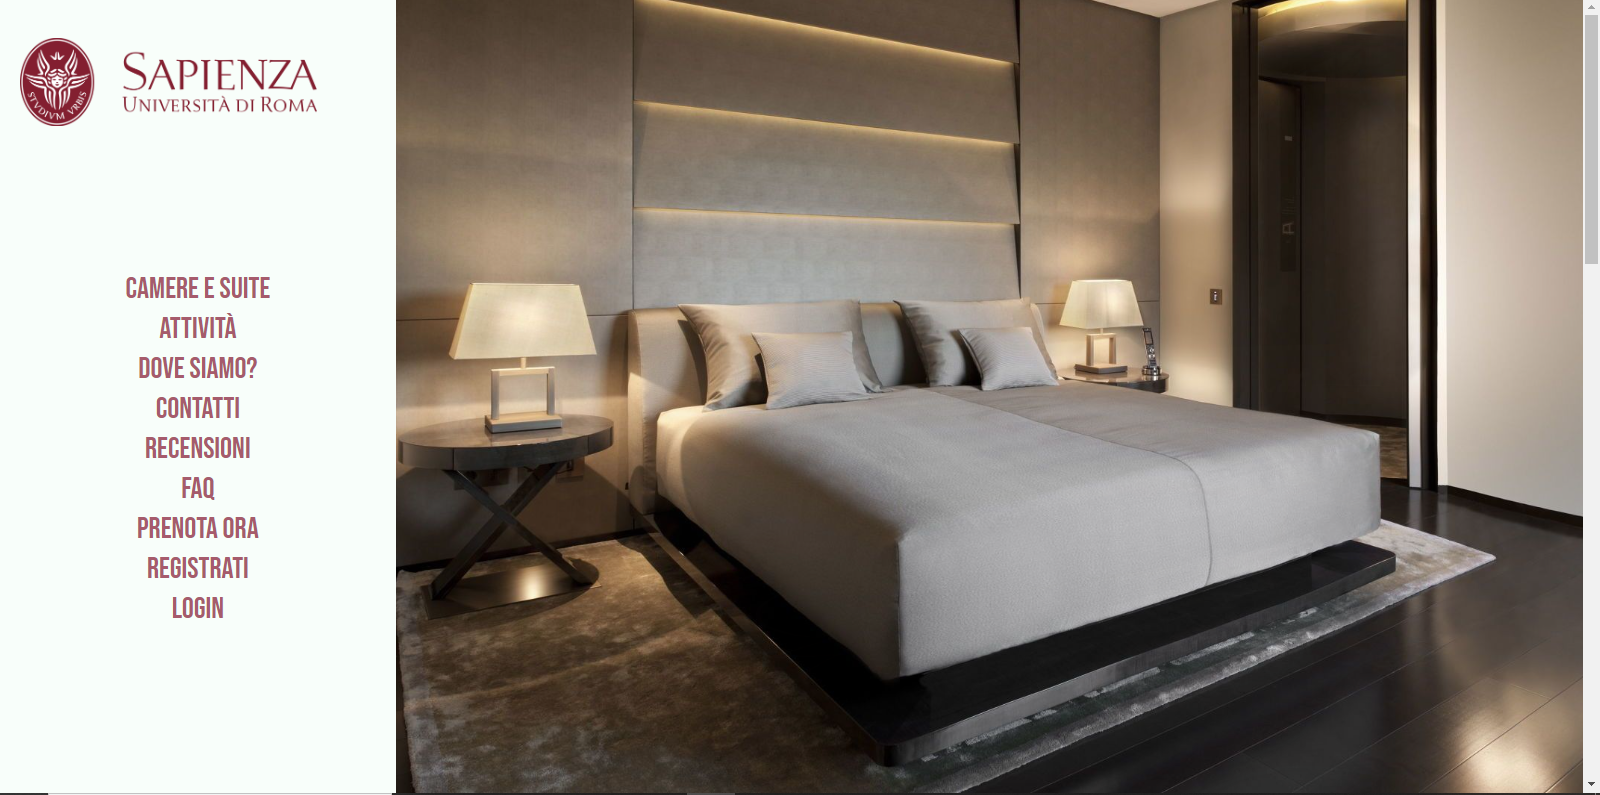
\includegraphics[scale=0.3]{HomePage.png}
\label{intro}
\caption{Homepage del sito}
\end{figure}\\
Tale pagina web è strutturata principalmente in \textbf{due sezioni verticali}, quella di sinistra e di destra. La sezione di destra è composta in \underline{quattro} \underline{sottosezioni orizzontali}: la prima dove vengono mostrate delle \textbf{immagini relative all'hotel} attraverso una animazione a scomparsa ,al di sotto si trovano le restanti sezioni nella quali vengono introdotte le \textbf{attività}, la \textbf{locazione} e i \textbf{contatti} dell'hotel.\\\\
Nella sezione di sinistra troveremo dei link con i quali l’utente potrà interagire cliccandoci sopra. Tra questi se ne possono trovare alcuni unicamente adibiti a scopo informativo che fanno riferimento a sezioni precise della pagina medesima, e sono: 
\begin{itemize}
\item \textbf{Attività:} la quale ci fornisce una piccola introduzione delle varie attività di cui potremmo usufruire avendo un soggiorno attivo.
\item \textbf{Dove siamo?:} fornisce indicazioni sulla locazione della struttura
\item \textbf{Contatti:} fornisce dei contatti di riferimento della struttura. 
\end{itemize}
I restanti link sono: camere e suite,  recensioni, faq, prenota ora, registrati e login. Le funzionalità dell'utente visitatore sono sei principalmente e le andremo ad analizzare più in dettaglio con i relativi link associati.

\medskip

\subsection{Visualizzare le camere e le suite}
\begin{figure}[h]
\centering 
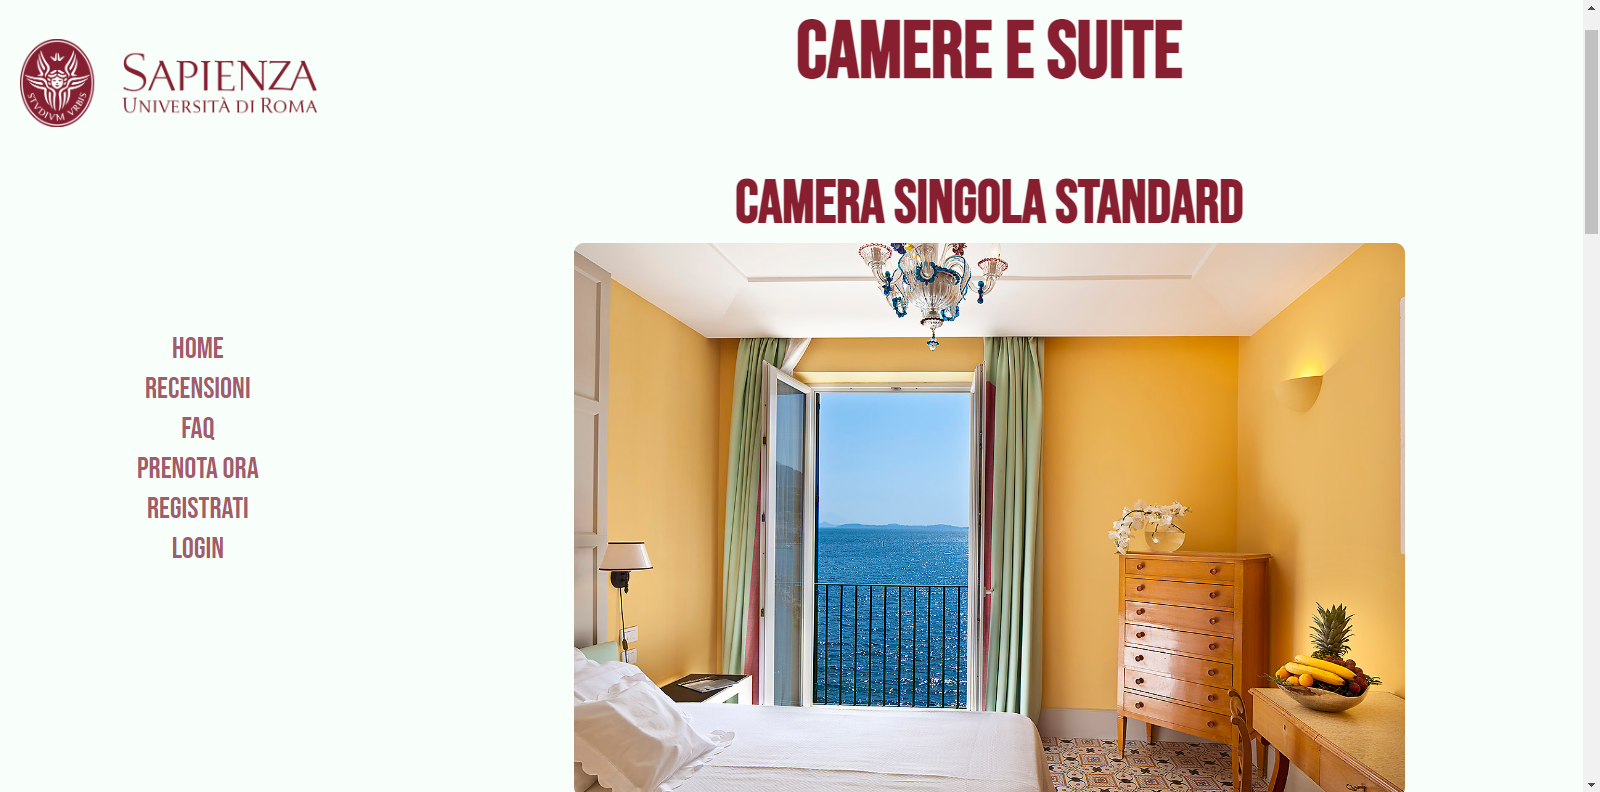
\includegraphics[scale=0.3]{Camere.png}
\caption{Camere e suite}
\label{Camere}
\end{figure}
Cliccando sul link denominato \textbf{"Camere e suite"} nella sezione sinistra della pagina, l'utente verrà indirizzato nella pagina mostrata in figura \ref{Camere}. La struttura della pagina è la stessa della homepage, con piccole differenze. La prima è che nella sezione di destra l'utente potrà prendere coscienza delle camere presenti all'interno della struttura con le relative informazioni associate ad ognuna di esse. La seconda è che nella sezione di sinistra troveremo solamente il link home, per tornare alla pagina principale dell'hotel ed i link delle recensioni, delle faq, della prenotazione di una camera, per la registrazione e per il login. 

\medskip

\subsection{Visualizzare le recensioni}
\begin{figure}[h]
\centering
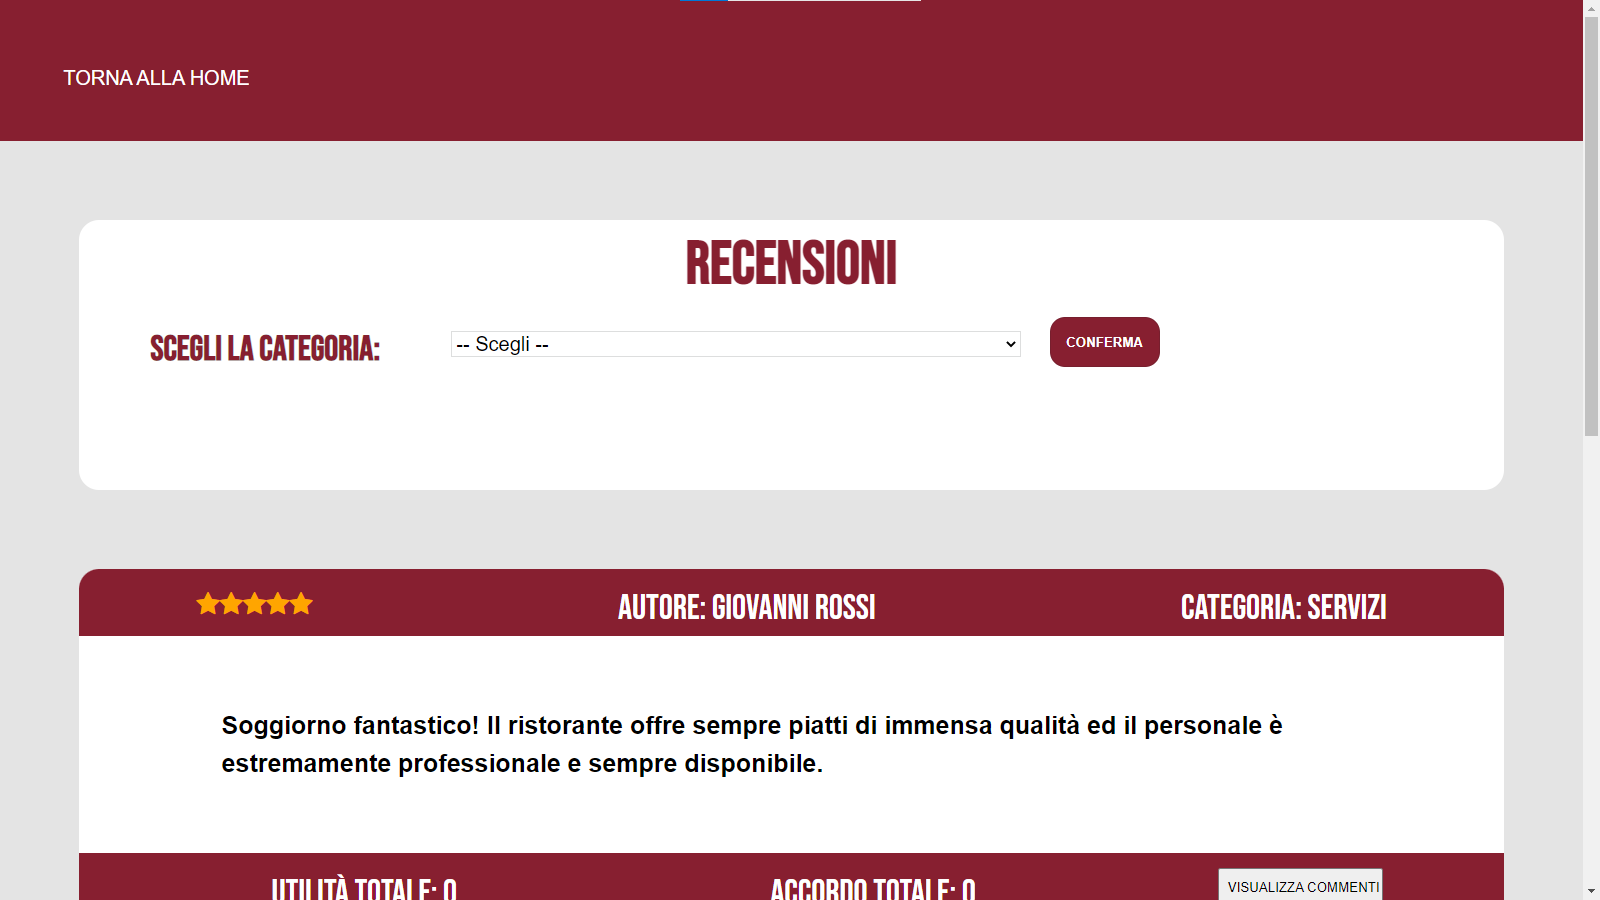
\includegraphics[scale=0.3]{RecensioniVisitatore.png}
\caption{Recensioni - visitatore}
\label{RecensioniVisitatore}
\end{figure}
Interagendo con il link \textbf{"Recensioni"} l'utente si ritroverà nella pagina rappresentata nella figura \ref{RecensioniVisitatore} In questa pagina potrà visionare  tutte le recensioni che sono state scritte dai clienti dell'hotel (cioè tutti utenti registrati all'interno del sito).\\\\
L'utente potrà visionare anche solamente le recensioni delle categorie che più lo interessano andando a selezionare la categoria dal menu a tendina presente nella parte superiore della pagina e andando a cliccare conferma.\\\\
L'utente visitatore avrà anche la possibilità di visualizzare tutti i commenti di risposta di una particolare recensione, andando a selezionare l'apposito pulsante \textbf{"visualizza commenti"} ed essere portato in una pagina come quella mostrata in figura \ref{RisposteRecensioneVisitatore} \newpage
\begin{figure}[h]
\centering
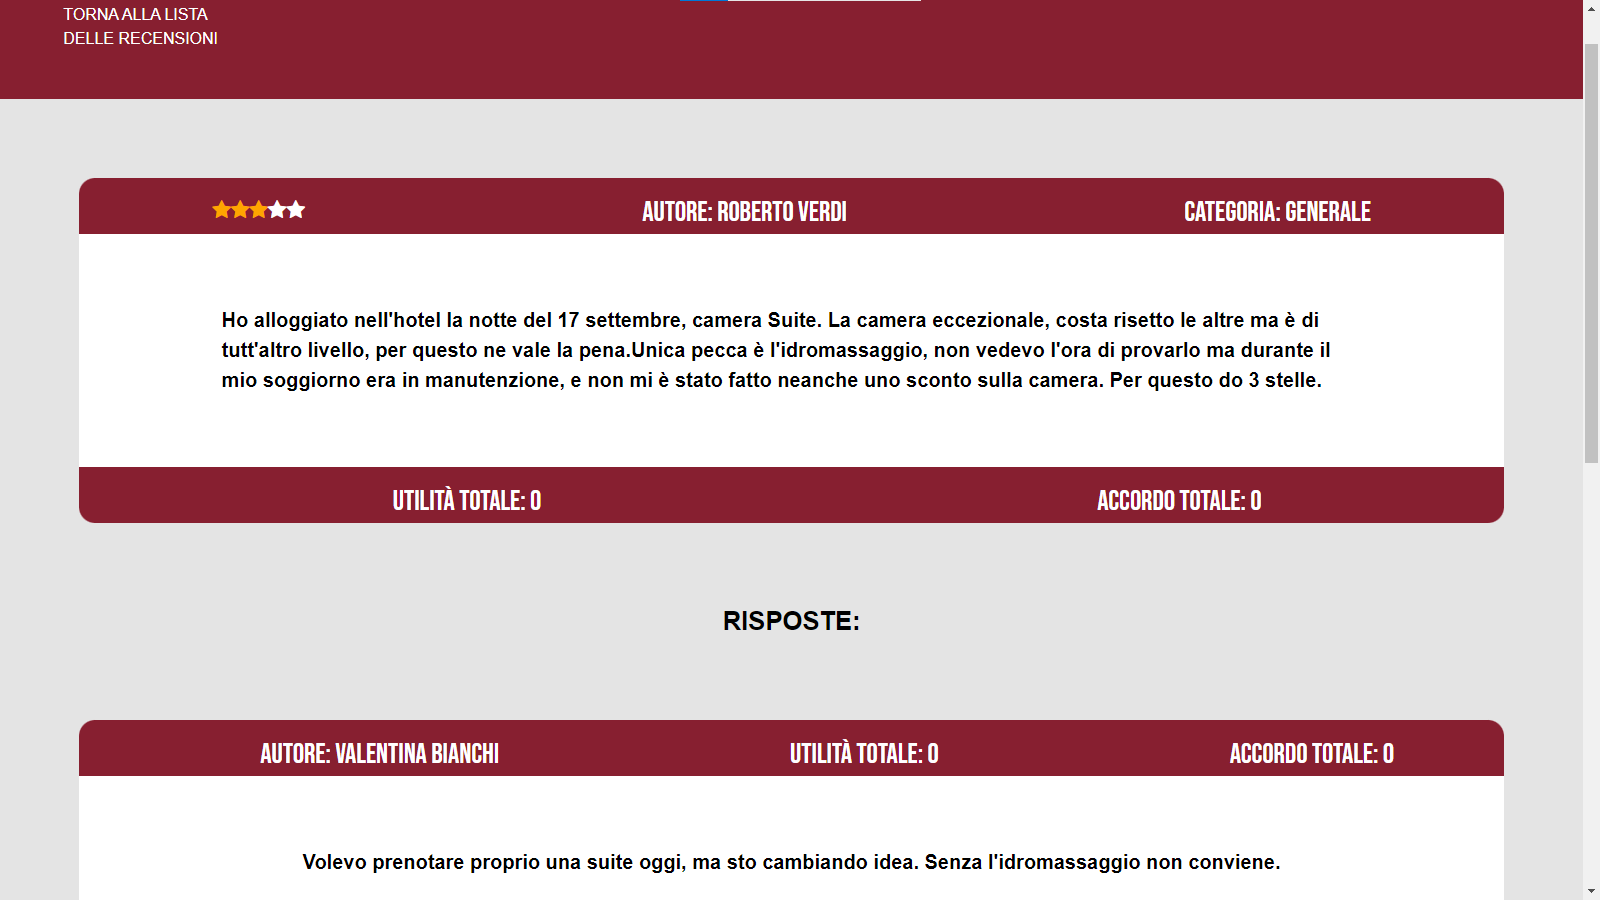
\includegraphics[scale=0.3]{RisposteRecensioneVisitatore.png}
\caption{Commenti di risposta di una recensione - visitatore}
\label{RisposteRecensioneVisitatore}
\end{figure}

\medskip

\subsection{Visualizzare le FAQ}
Nella pagina delle Faq, figura \ref{FaqVisitatore} , accessibile attraverso l'interazione del link presente in home denominato \textbf{"FAQ"}, l'utente è in grado di visionare tutte le Faq dell'hotel che, per definizione, sono delle domande di rilevante importanza e di maggiore frequenza tra l'utenza della piattaforma.
\begin{figure}[!ht]
\centering
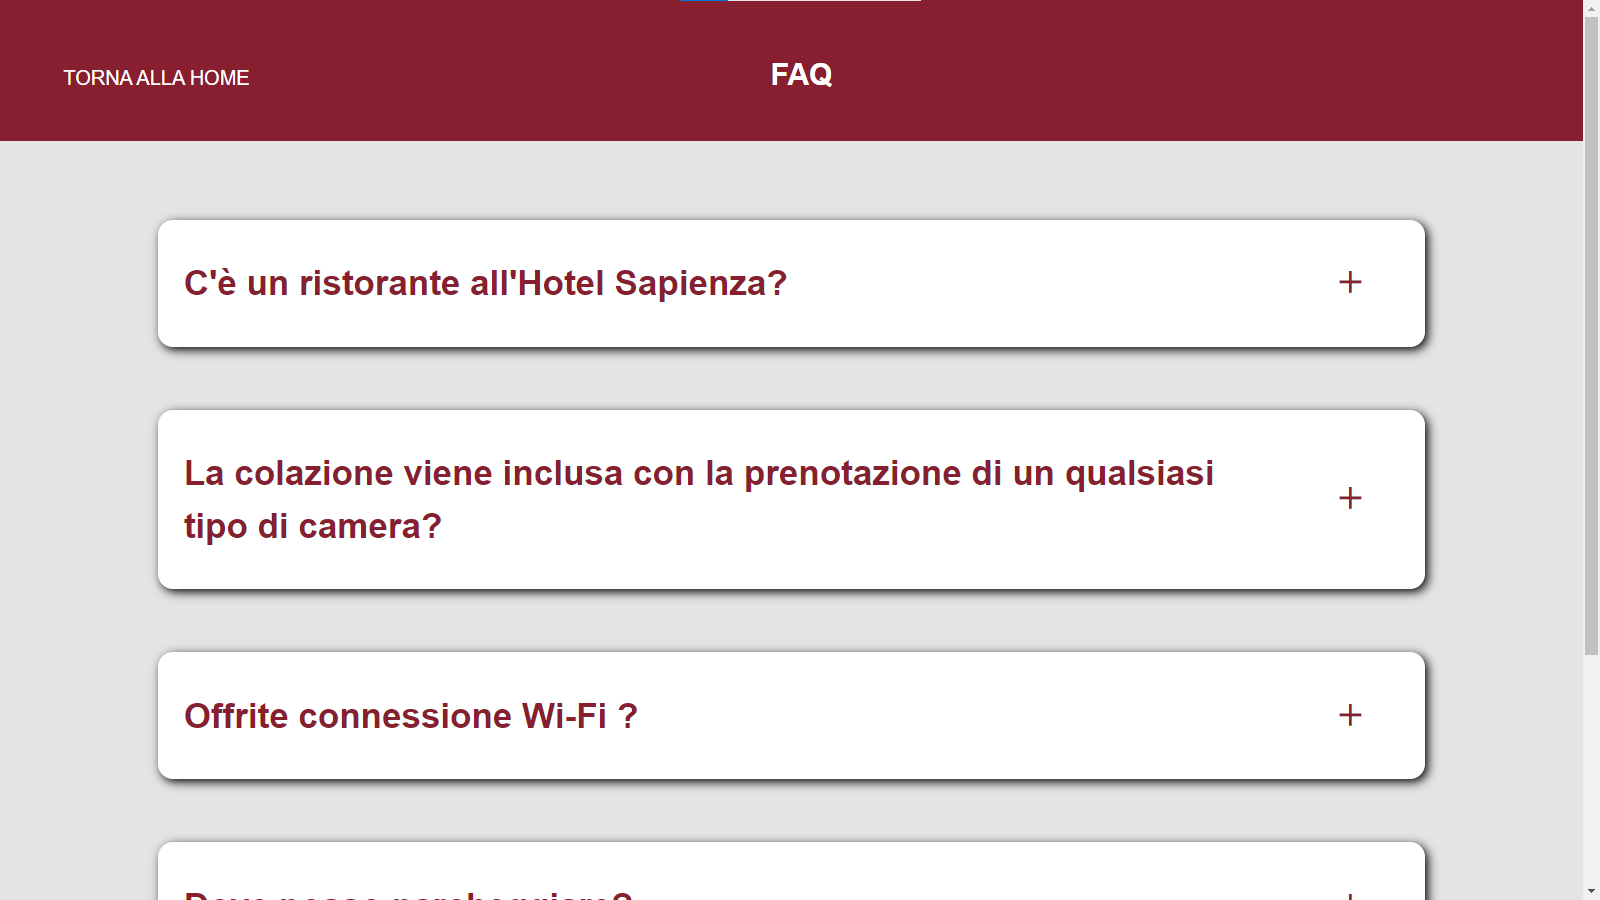
\includegraphics[scale=0.29]{FaqVisitatore.png}
\caption{Pagina delle FAQ}
\label{FaqVisitatore}
\end{figure}

\subsection{Prenotazione di un soggiorno}
Cliccando su \textbf{"PRENOTA ORA"} l'utente viene indirizzato nella pagina riportata nella figura \ref{PrenotaOra} nella quale potrà selezionare una data di arrivo e una di partenza; una volta selezionate le date e cliccato sul bottone \textbf{"verifica disponibilità"}, sarà indirizzato in una nuova pagina, figura \ref{VisualizzaDisponibilita}, dove vengono mostrate le camere disponibili nelle date selezionate con relativo prezzo. Andando a selezionarne una, l'utente verrà indirizzato forzatamente nella pagina di login, riportata nella figura \ref{LoginPrenotazione}, nella quale dovrà autenticarsi per poter completare la prenotazione del soggiorno, o annullare la prenotazione
\begin{figure}[h]
\centering
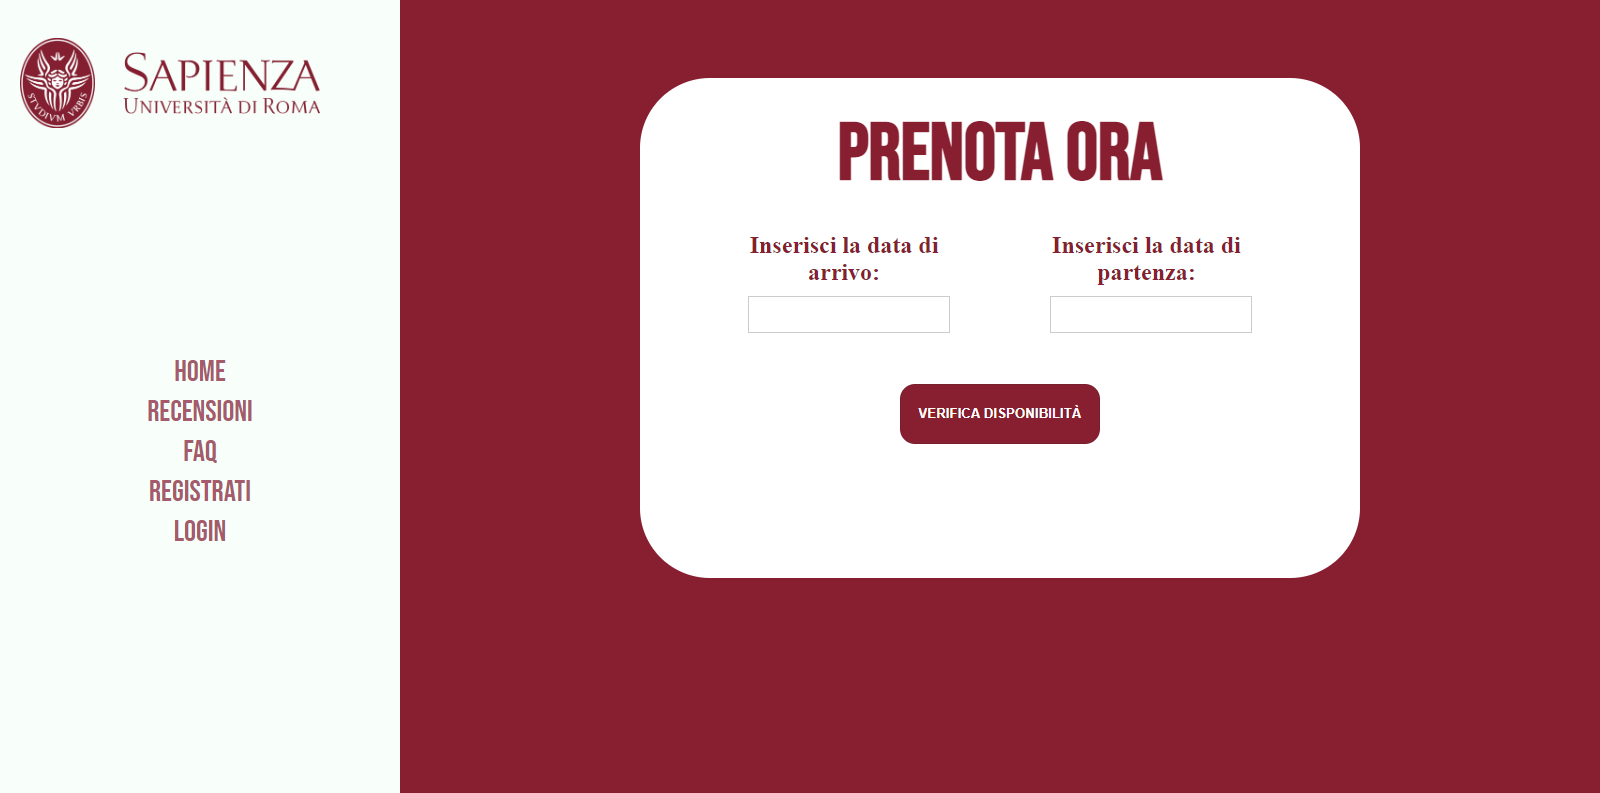
\includegraphics[scale=0.3]{PrenotaOra.png}
\caption{Prenotazione di un soggiorno}
\label{PrenotaOra}
\end{figure}

\begin{figure}[h]
\centering
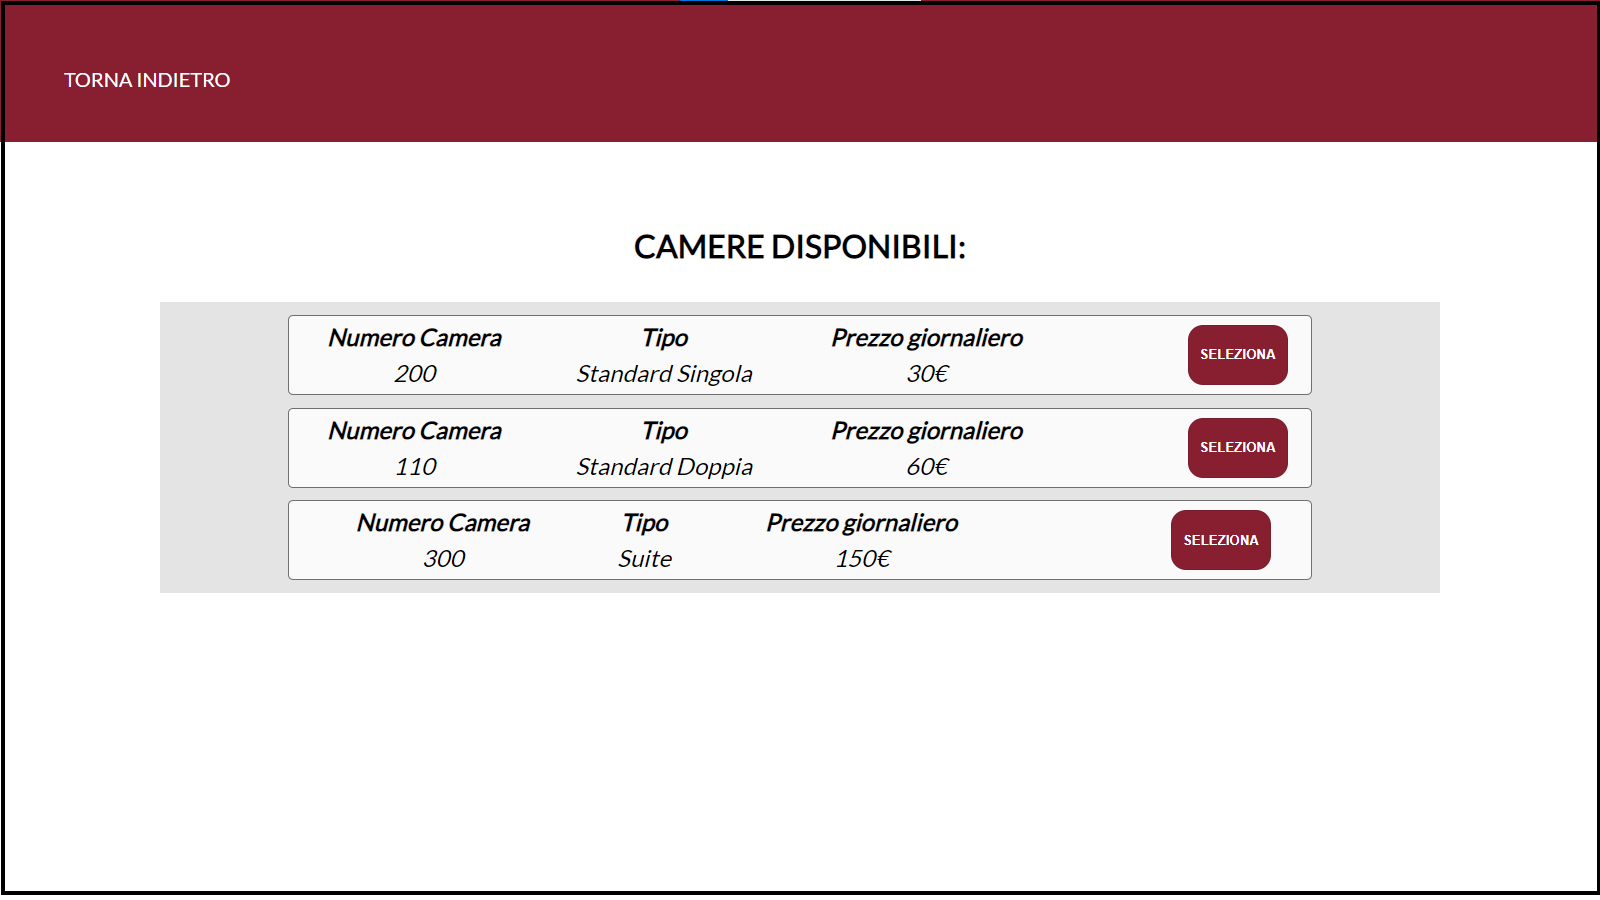
\includegraphics[scale=0.24]{VisualizzaDisponibilita.png}
\caption{Camere disponibili}
\label{VisualizzaDisponibilita}
\end{figure}\newpage

\begin{figure}[h]
\centering
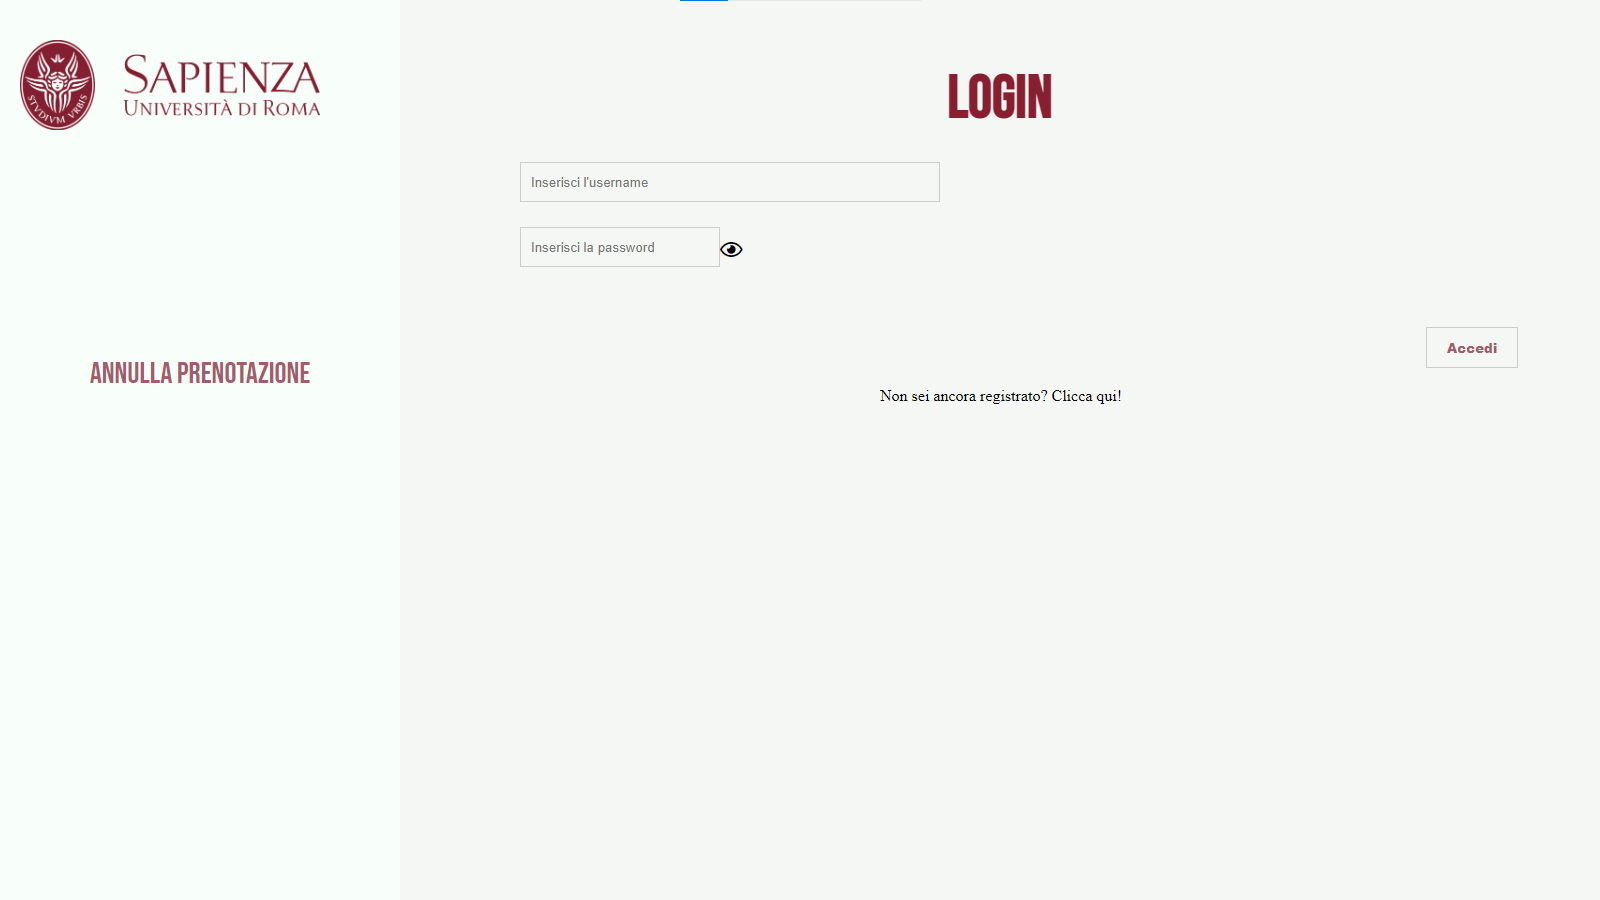
\includegraphics[scale=0.3]{LoginPrenotazione.png}
\caption{Login utente durante la prenotazione di una camera}
\label{LoginPrenotazione}
\end{figure}

\subsection{Autenticarsi}
\begin{figure}[!ht]
\centering
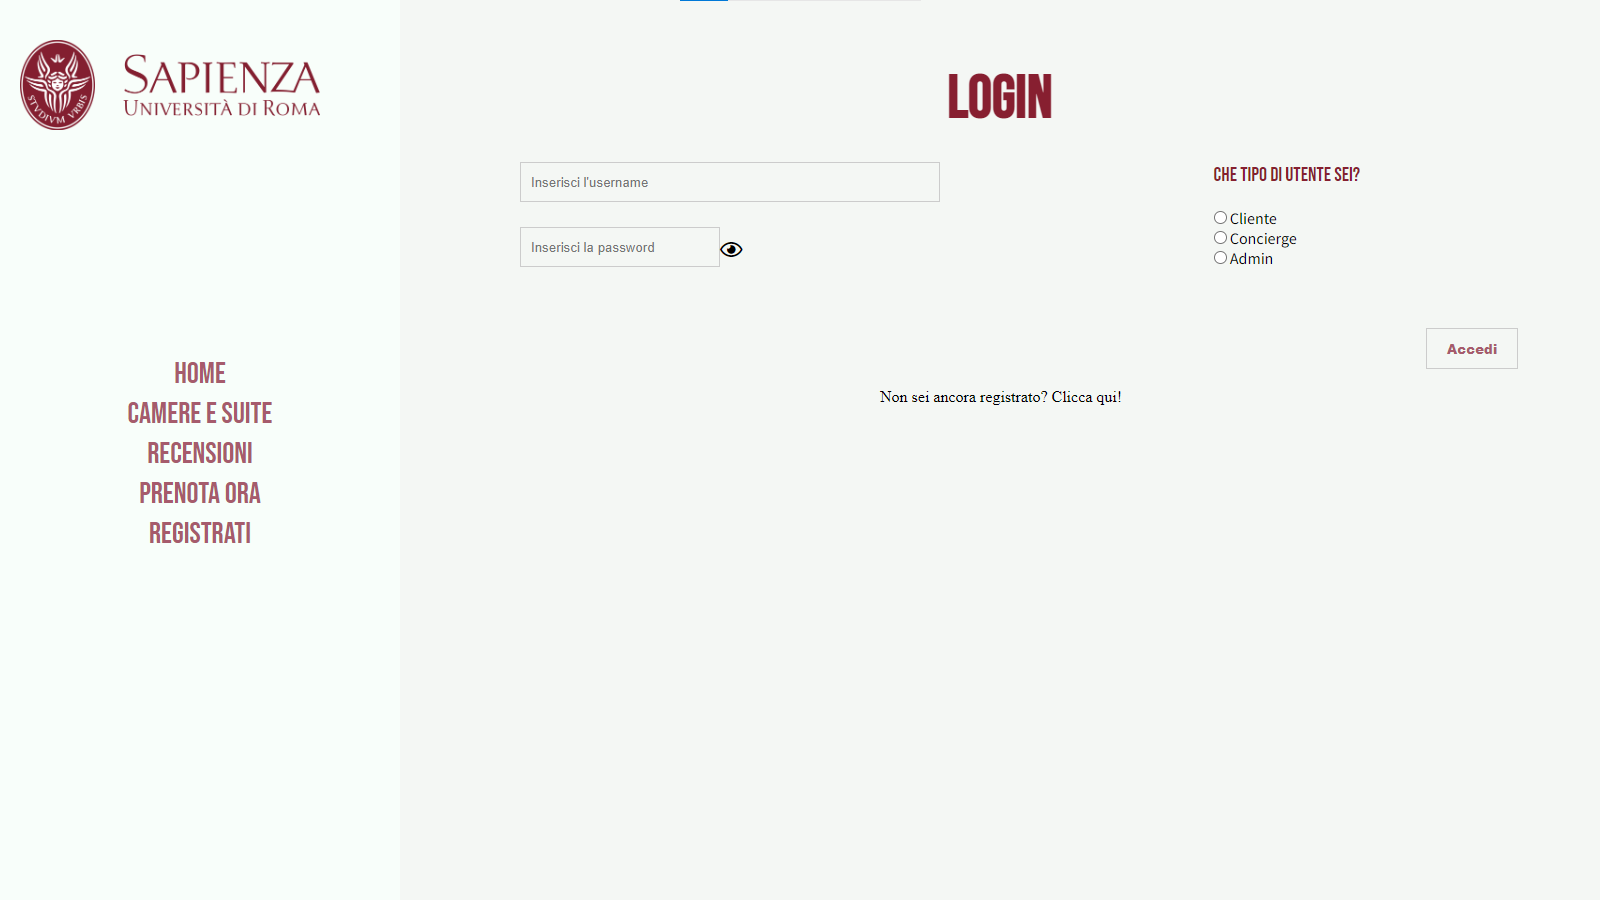
\includegraphics[scale=0.3]{Login.png}
\caption{Pagina di login}
\label{LoginNormale}
\end{figure}
L'utente visitatore potrà autenticarsi così da cambiare tipo di utenza e passare a quella di \textbf{"Cliente"} nella pagina di login, figura \ref{LoginNormale}, accessibile o dalla sezione sinistra della home attraverso l'interazione con il link\pagebreak \textbf{"LOGIN"} o attraverso la prenotazione di un soggiorno come descritto nel paragrafo 2.1.4. \\\\
Se si accede dalla home, la pagina risulterà lievemente differente, come rappresentato nella figura \ref{LoginNormale}, ovvero si richiederà all’utente visitatore di specificare il suo \underline{tipo di utenza} tra cliente, admin e concierge. È logico presumere che l'utente si autentifichi come cliente solamente dopo essersi registrato alla piattaforma. Per l'autenticazione, inoltre, l'utente deve inserire il proprio \textbf{username} e la propria \textbf{password}.\\\\
Una volta autenticato, l'utente cesserà di essere un semplice visitatore, potendo usufruire di tutte le ulteriori funzionalità che la propria tipologia di utenza le mette a disposizione. 

\subsection{Registrazione}
\begin{figure}[h]
\centering
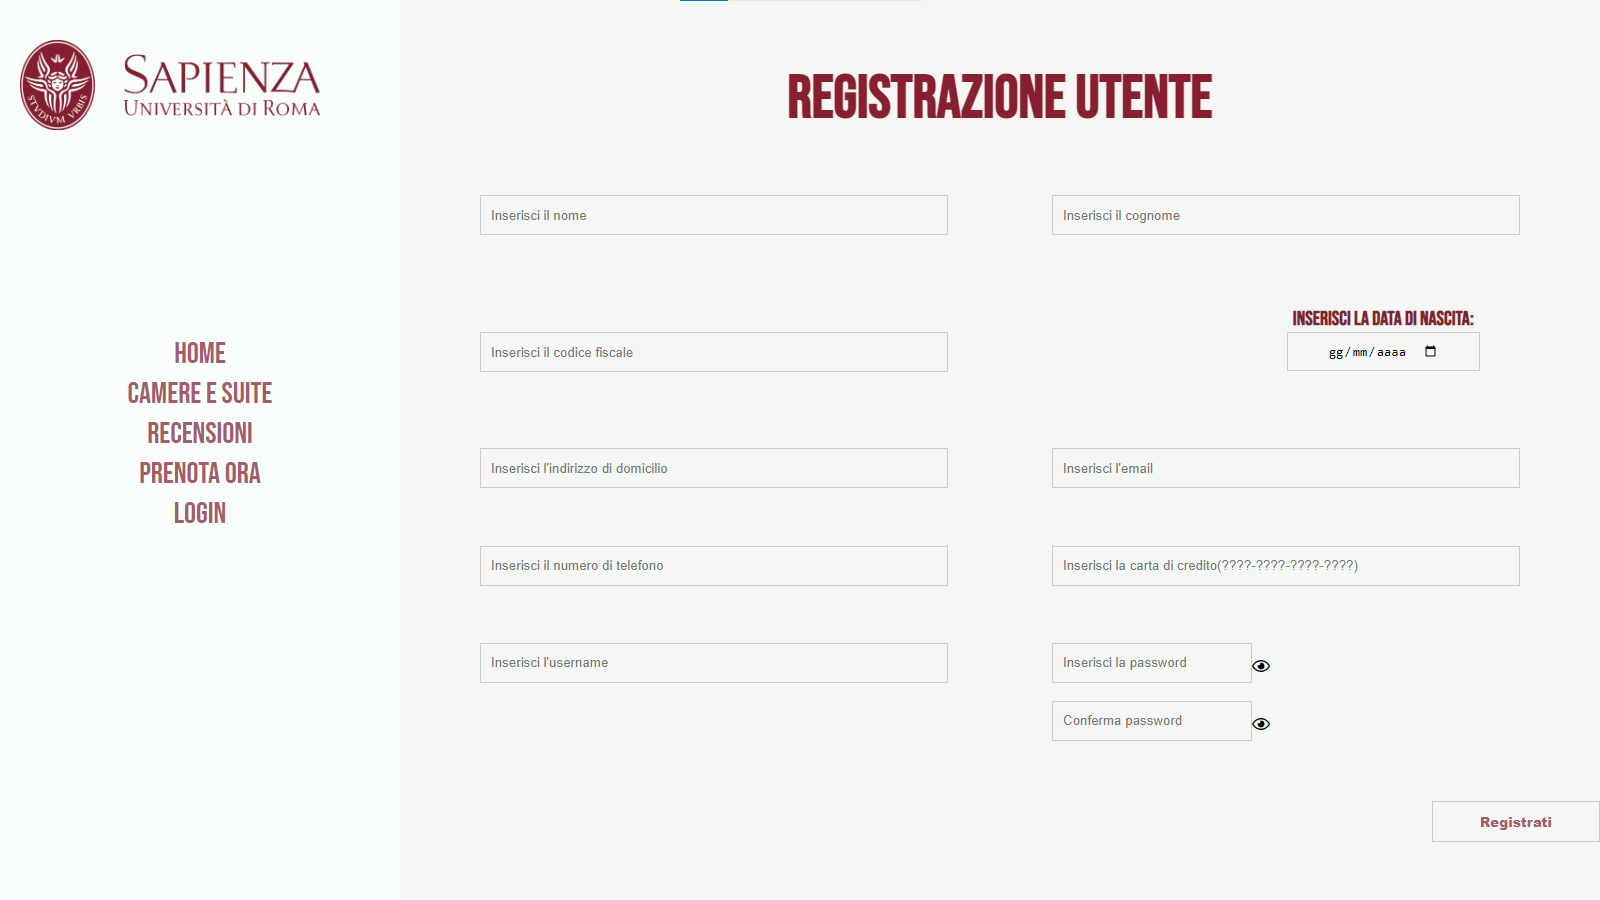
\includegraphics[scale=0.3]{Registrazione.png}
\caption{Pagina di registrazione}
\label{Registrazione}
\end{figure}
Qualora l'utente non disponesse delle credenziali per poter effettuare il login ma vorrebbe comunque poter usufruire delle funzionalità della tipologia cliente, non gli resta che registrarsi alla piattaforma attraverso il link \textbf{"REGISTRAZIONE"} presente nella sezione sinistra della home. Una volta arrivato nella pagina della registrazione utente, figura \ref{Registrazione}, l'utente non deve far altro che compilare tutti i campi mostrati nella pagina con i propri dati e cliccare sul bottone \textbf{"Registrati"} in basso a destra. Se la procedura prosegue senza alcun problema durante la compilazione della pagina, allora l'utente sarà a tutti gli effetti registrato all'interno della piattaforma e verrà reindirizzato alla pagina di login mostrata in figura \ref{LoginNormale}.

\medskip
\medskip

\section{Cliente}
In questa sezione andiamo ad analizzare tutte le funzionalità usufruibili da un tipo di utenza \textbf{"Cliente"}.\\\\
Assumiamo quindi che il nostro utente si sia prima di tutto autenticato attraverso la pagina di login come descritto nel paragrafo 2.1.5. Come schermata iniziale, il cliente si troverà una home identica a quella dell'utente visitatore con delle piccole differenze riguardo ai link accessibili sulla sezione verticale sinistra della pagina, come mostrato nella figura \ref{HomePageCliente}. Notiamo che il link \textbf{"LOGIN"} è stato sostituito dal link \textbf{"LOGOUT"}, è stato rimosso il link \textbf{"REGISTRATI"} e il prenota ora è presente solamente se il cliente risulti non avere neanche un soggiorno attivo. 
Il cliente gode altrettanto delle funzionalità dell'utente visitatore, escluse quelle dell'autenticazione e della registrazione.\\\\
Se il cliente non risulta avere tra i propri soggiorni, nemmeno uno con lo stato di soggiorno attivo, allora potrà godere unicamente delle funzionalità della prenotazione di un soggiorno, della visualizzazione dei propri dati con relativa modifica, della visualizzazione delle proprie prenotazioni, del menù e delle attività messe a disposizione dall'hotel.
\begin{figure}[!h]
\centering
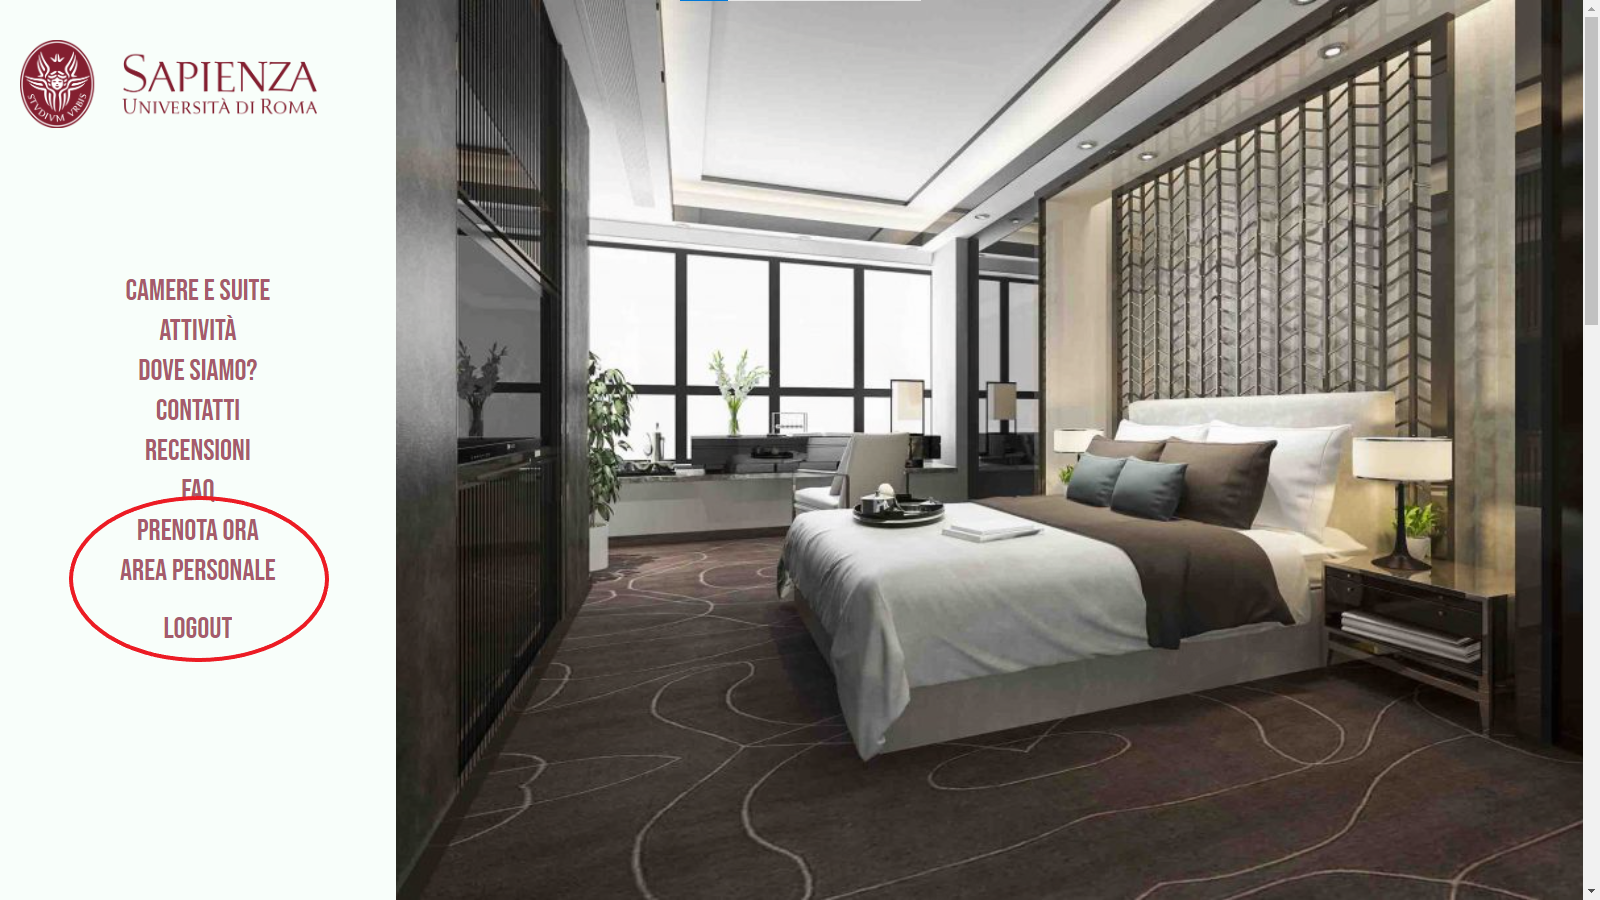
\includegraphics[scale=0.24]{HomePageCliente.png}
\caption{Homepage del sito - Cliente}
\label{HomePageCliente}
\end{figure}\newpage

\subsection{Accedere all'area cliente}
\begin{figure}[!h]
\centering

\includegraphics[scale=0.3]{AreaCliente.png}
\caption{Area cliente}
\label{AreaCliente}
\end{figure}
Dalla schermata iniziale il cliente può essere indirizzato nella propria area cliente, figura \ref{AreaCliente}, interagendo con il link \textbf{"AREA PERSONALE"}. La struttura della pagina è la stessa della homepage, ora però sul lato sinistro troviamo tutti quei link che rappresentano le vere e proprie funzionalità di un cliente. Tuttavia, come già detto, le funzionalità di un cliente dipendono molto dallo stato del soggiorno del cliente presso l'hotel.\\\\
Naturalmente cliccando il link \textbf{"HOME"} si ritorna alla schermata principale mostrata in figura \ref{HomePageCliente}

\subsection{Prenotare un soggiorno}
Il cliente che non risulta avere un soggiorno con stato pagamento approvato o con pagamento sospeso (ovvero un soggiorno attivo) potrà effettuare una prenotazione di un soggiorno attraverso il link \textbf{"PRENOTA ORA"}. Il procedimento è lo stesso descritto nella sottoparagrafo 2.1.4, con l'unica eccezione che una volta selezionata la camera disponibile e desiderata nella figura \ref{VisualizzaDisponibilita}, il cliente essendo già autentificato, non verrà più indirizzato nella pagina di login ma in una pagina conferma prenotazione, dove vengono riassunte tutte le informazioni riguardo la prenotazione con relativo prezzo totale. È qui che, se il cliente risulta essere in possesso di crediti, può utilizzarli per ricevere uno sconto sul prezzo totale del soggiorno. Un esempio viene mostrato nella figura \ref{ConfermaPrenotazioneCamera}. Il cliente qui può decidere se annullare la prenotazione o di confermarla. Nel secondo caso verrà portato in una pagina che lo assicura che la prenotazione del soggiorno è andata a buon fine, la pagina risulta essere come quella nella figura \ref{PrenotazioneCompletata}.  In questa pagina il cliente non deve fare altro che attendere per qualche secondo così da essere indirizzato automaticamente nell'area cliente. Ora il cliente dovrà attendere che il pagamento sia approvato dall'admin per poter usufruire di tutte le funzionalità di un cliente con un soggiorno approvato.
\begin{figure}[!h]
\centering
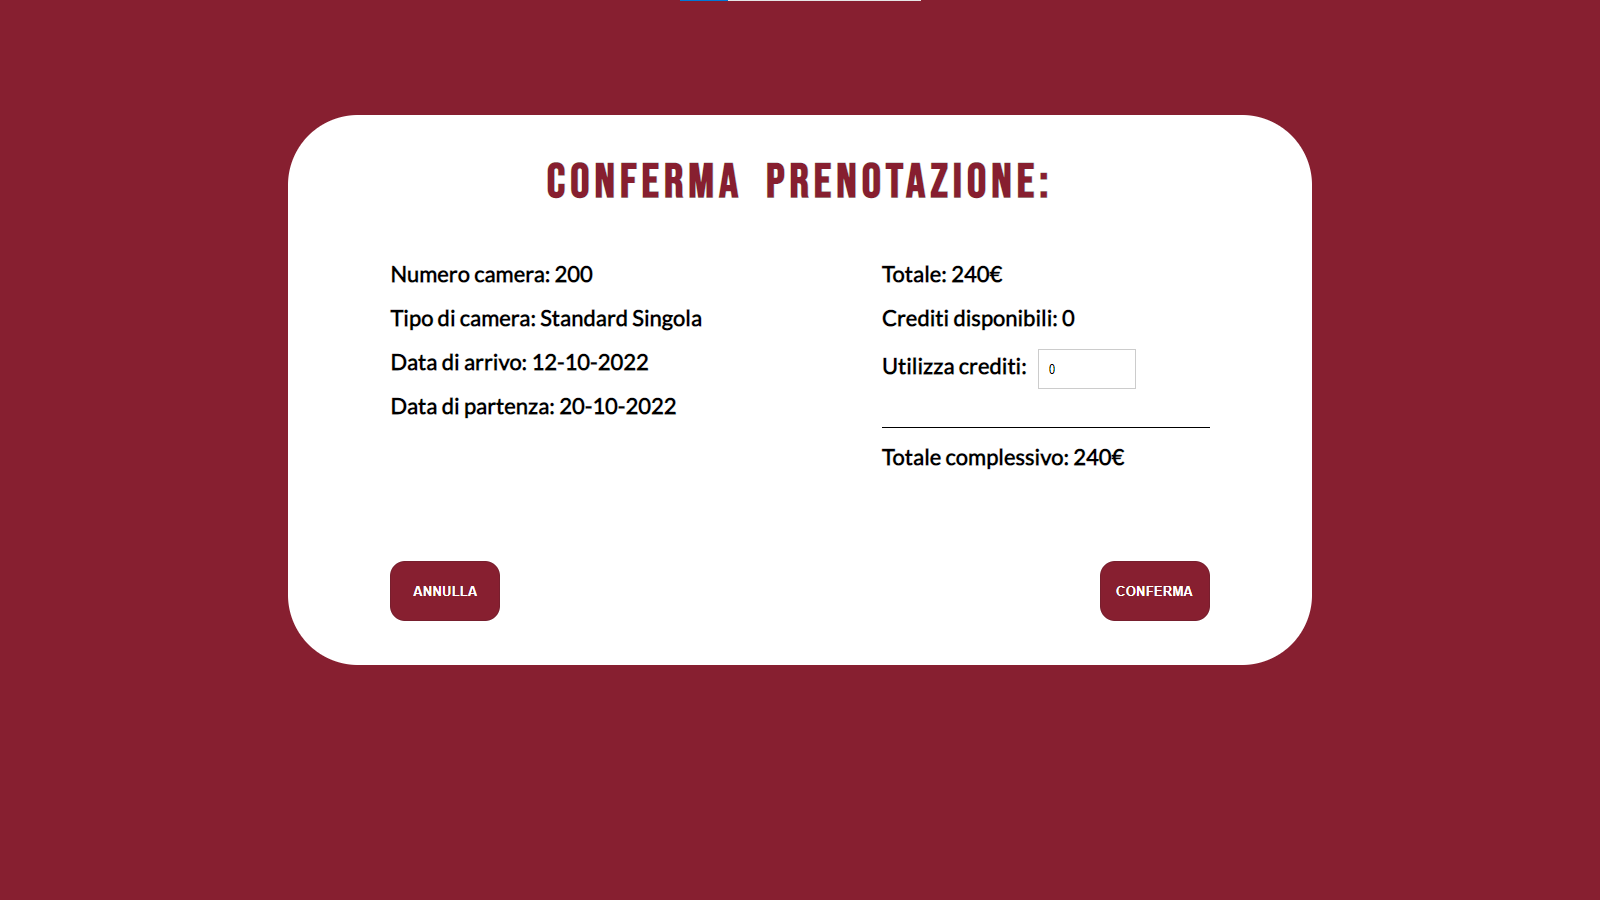
\includegraphics[scale=0.3]{ConfermaPrenotazioneCamera.png}
\caption{Conferma prenotazione di un soggiorno presso l'hotel}
\label{ConfermaPrenotazioneCamera}
\end{figure}
\begin{figure}[!h]
\centering

\includegraphics[scale=0.26]{PrenotazioneCompletata.png}
\caption{Prenotazione completata}
\label{PrenotazioneCompletata}
\end{figure}

\subsection{Prenotare un tavolo}
Se il cliente risulta avere un soggiorno approvato, cliccando su \textbf{"SERVIZIO DI RISTORAZIONE"}, il cliente viene indirizzato nella pagina del servizio di ristorazione, rappresentata nella figura \ref{HomepageRistorante}. Cliccando ora sul link \textbf{"PRENOTA TAVOLO"} nella sezione verticale sinistra della pagina il cliente può accedere ad una specifica pagina, figura \ref{PrenotaTavolo}, nella quale potrà effettuare la prenotazione di un tavolo. Qui dovrà inserire i dati nei vari campi, tra i quali la \underline{data di prenotazione}. (ovviamente saranno mostrate disponibili solamente le date comprese nel soggiorno approvato del cliente), la \underline{locazione} (interna o esterna), selezionare tra pranzo e cena e scegliere un \underline{orario} tra quelli proposti. Una volta inseriti tutti i campi e cliccato sul bottone di conferma il cliente visionerà la solita schermata di attesa che lo assicura che la prenotazione sia andata a buon fine e verrà automaticamente reindirizzato nell'area cliente pochi secondi dopo. 
\begin{figure}[!h]
\centering
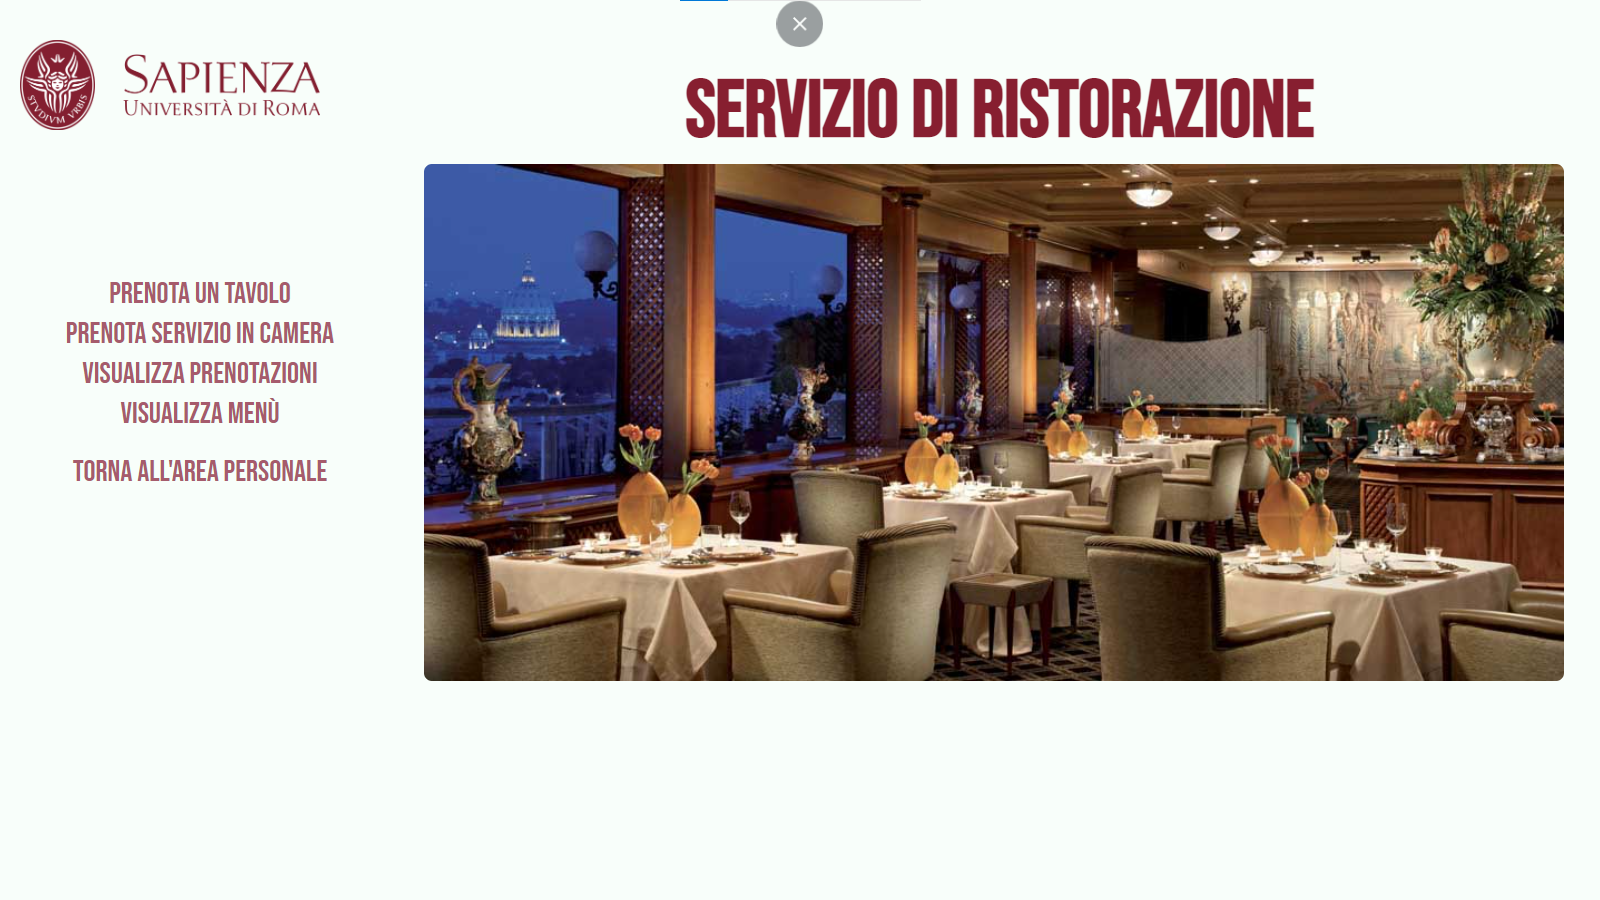
\includegraphics[scale=0.33]{HomepageRistorante.png}
\caption{Homepage del servizio di ristorazione}
\label{HomepageRistorante}
\end{figure}\newpage
\begin{figure}[!h]
\centering
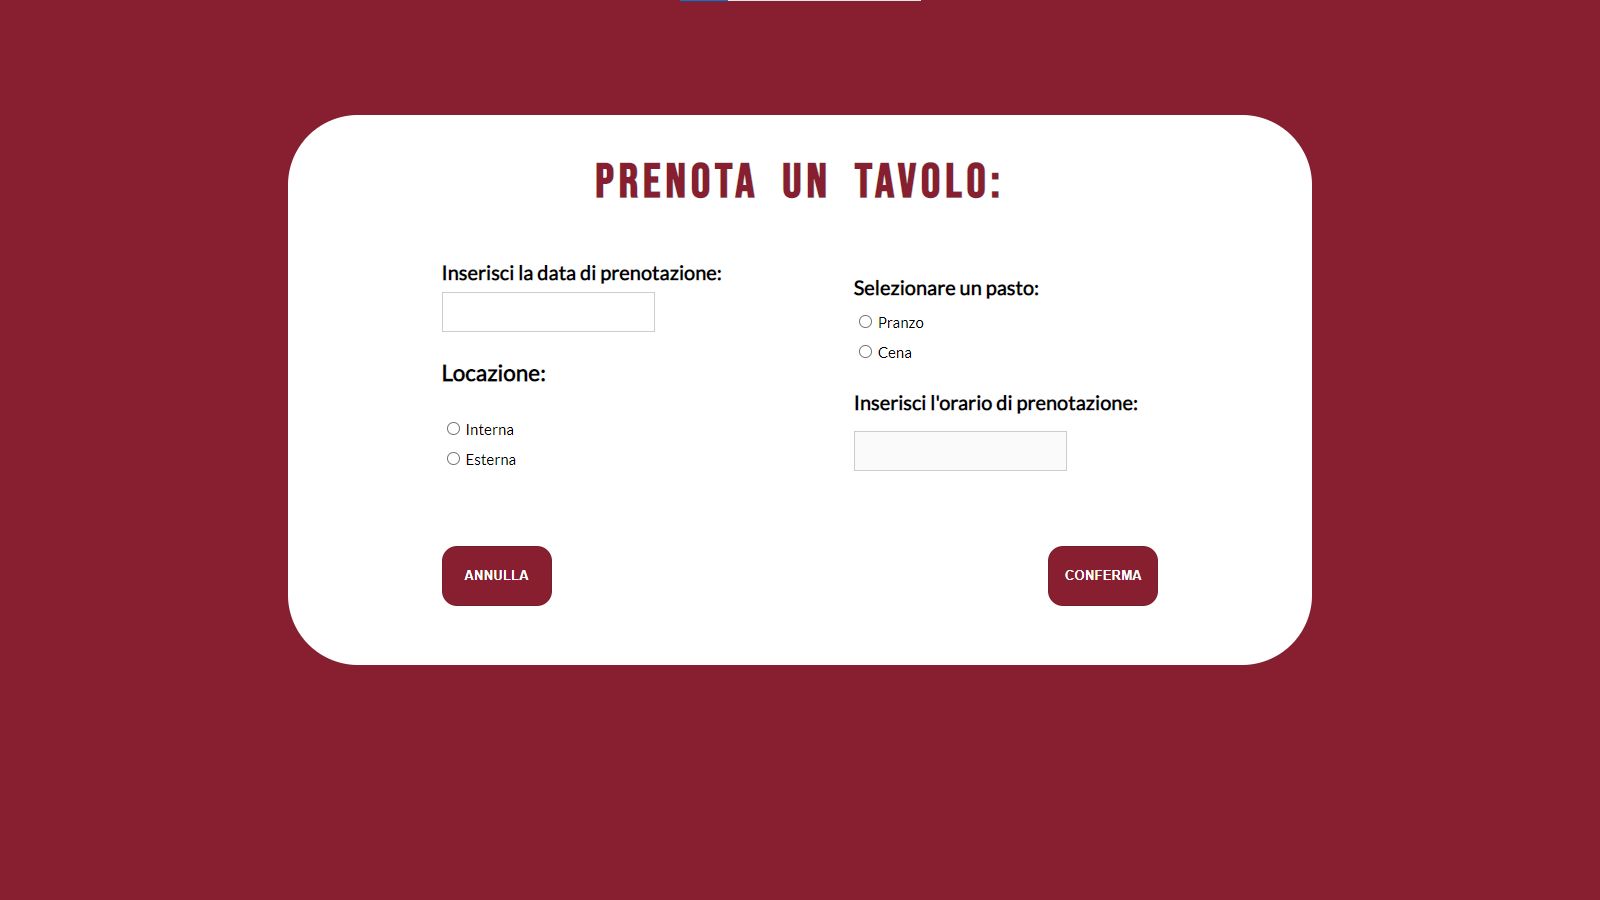
\includegraphics[scale=0.3]{PrenotaTavolo.png}
\caption{Pagina di prenotazione di un servizio al tavolo}
\label{PrenotaTavolo}
\end{figure}

\subsection{Prenotare un servizio in camera}
Oltre a prenotare un tavolo, se il cliente risulta avere un soggiorno approvato, nella pagina del servizio di ristorazione può prenotare un servizio in camera. Se il menù non è in fase di aggiornamento, allora il cliente interagendo con il link \textbf{"PRENOTA UN SERVIZIO IN CAMERA"} verrà portato nella pagina, mostrata nella figura \ref{PrenotaSC}, dove dovrà inserire il \underline{giorno del servizio in camera} (i giorni che può selezionare sono quelli compresi nel suo soggiorno approvato), selezionare tra pranzo e cena e scegliere un \underline{orario}. Ora l'utente può confermare le scelte e proseguire con la prenotazione oppure tornare indietro nell'area del servizio di ristorazione. Nel primo caso verrà mostrato al cliente il menù, come in figura \ref{ScegliPortateSC}, nel quale l'utente potrà selezionare le \underline{portate desiderate con le relative quantità} e aggiungere anche delle \underline{richieste aggiuntive}. Anche qui viene mostrata la possibilità al cliente di annullare o proseguire la prenotazione. Se si sceglie di proseguire, il cliente troverà un sommario delle informazioni relative alla prenotazione con la possibilità di poter utilizzare dei crediti per riceve uno sconto sul prezzo totale (se disponibili). Un esempio lo si può trovare raffigurato nella figura \ref{ConfermaPrenotazioneSC}. In caso di conferma della prenotazione il cliente verrà indirizzato nella pagina di conferma avvenuta prenotazione e pochi secondi dopo si ritroverà nuovamente nell'area cliente\newpage
\begin{figure}[!h]
\centering
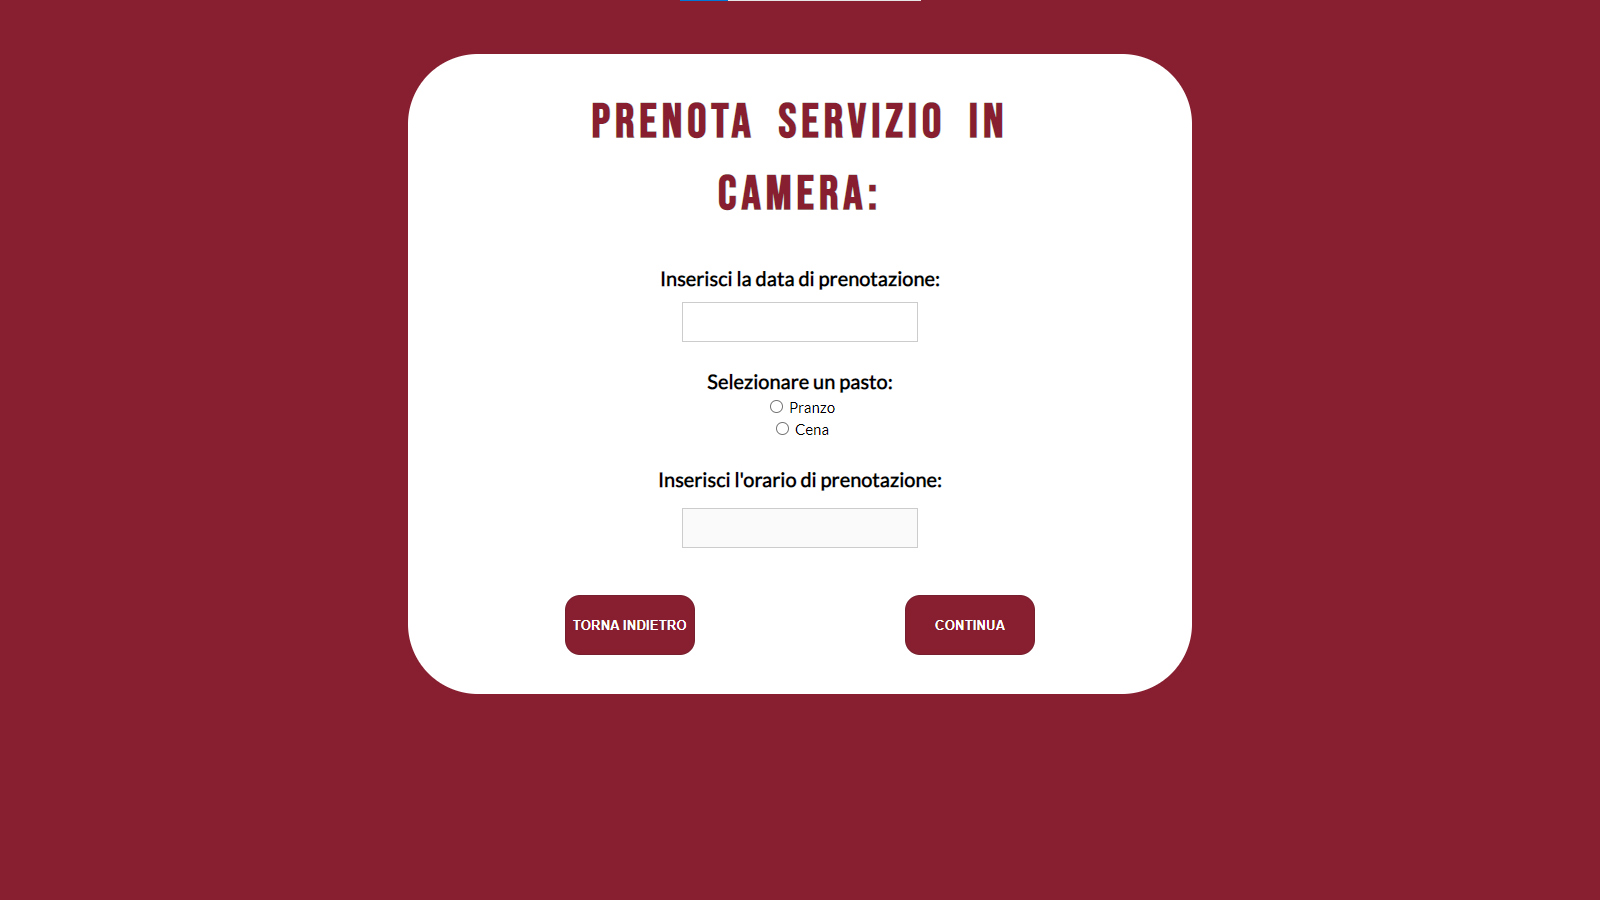
\includegraphics[scale=0.3]{PrenotaSC.png}
\caption{Pagina per inserire la data e l'orario del servizio in camera}
\label{PrenotaSC}
\end{figure}
\begin{figure}[!h]
\centering
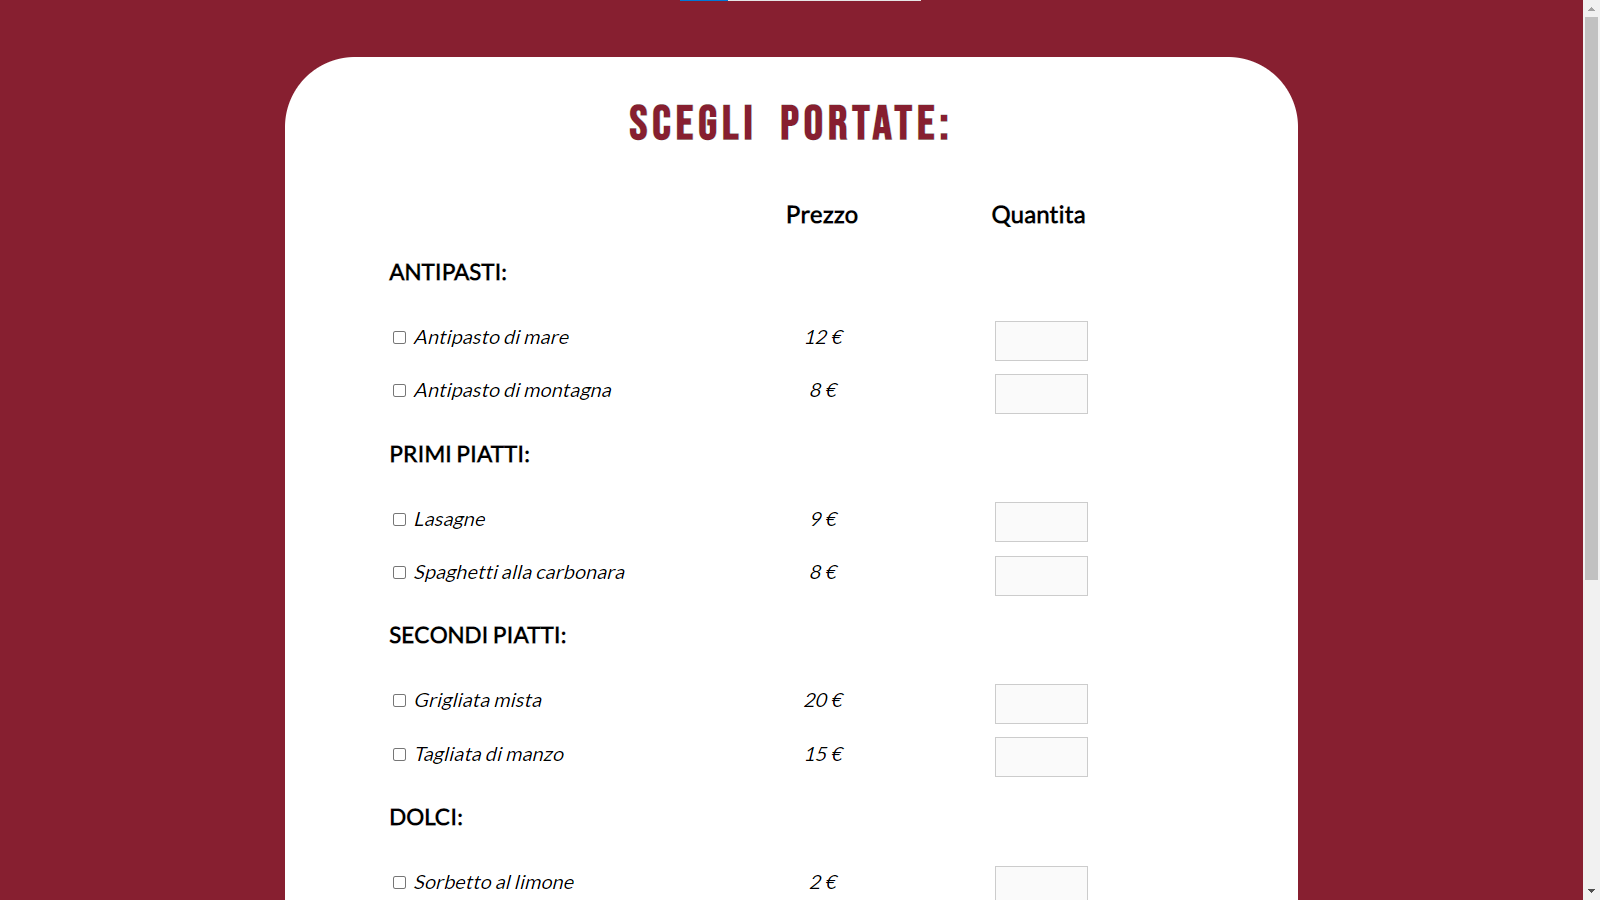
\includegraphics[scale=0.3]{ScegliPortateSC.png}
\caption{Scelta delle portate per il servizio in camera}
\label{ScegliPortateSC}
\end{figure}\newpage
\begin{figure}[!h]
\centering
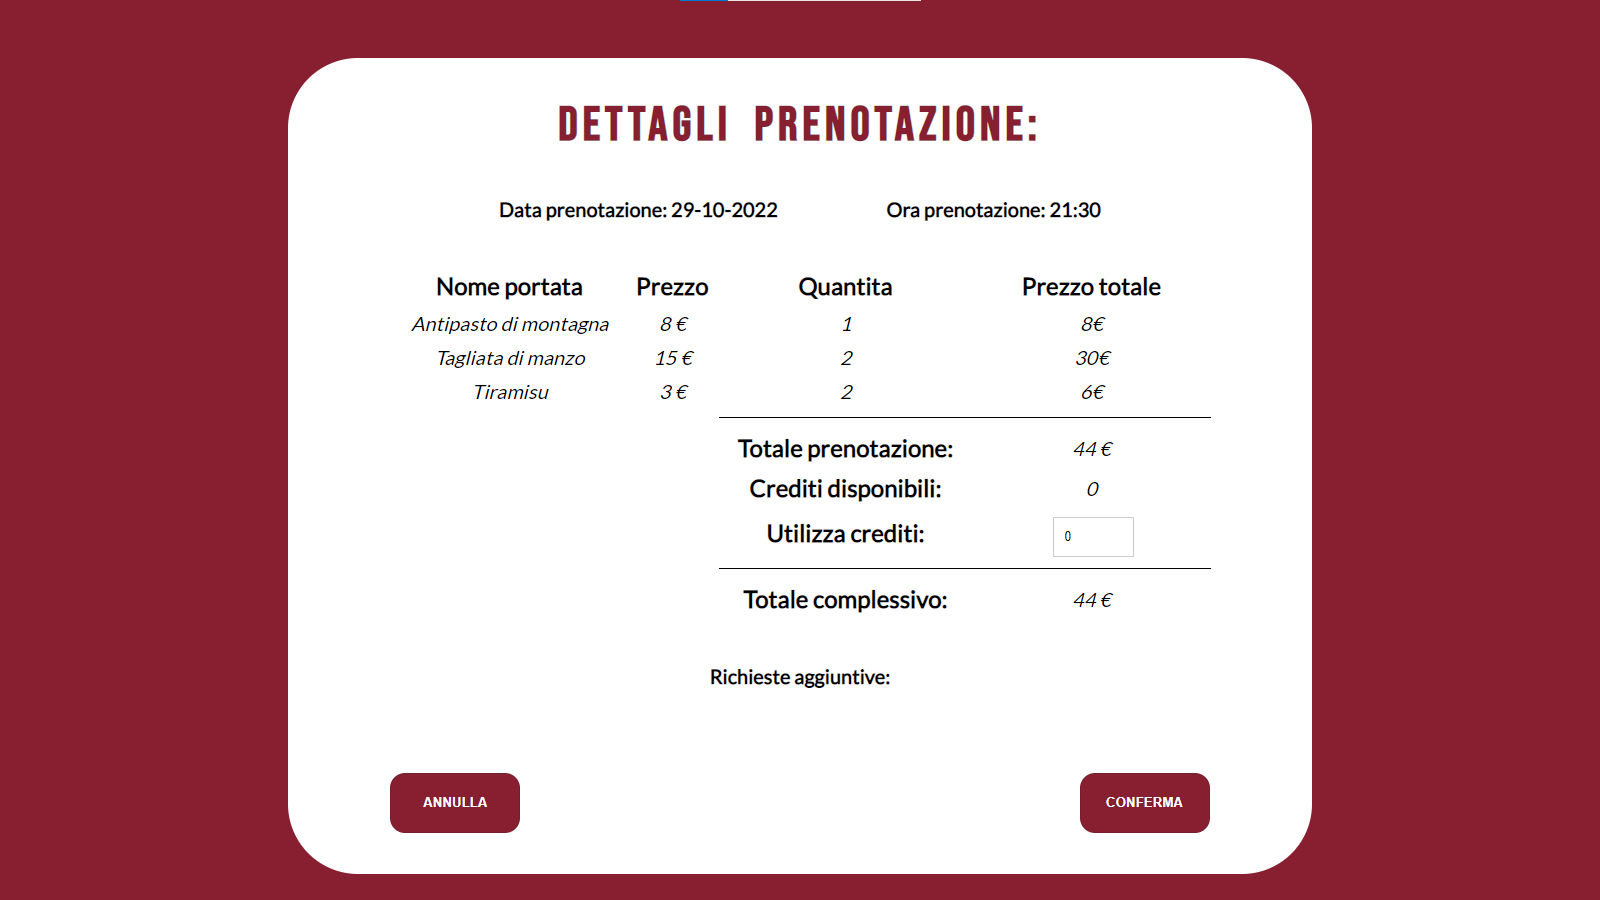
\includegraphics[scale=0.3]{ConfermaPrenotazioneSC.png}
\caption{Conferma prenotazione di un servizio in camera}
\label{ConfermaPrenotazioneSC}
\end{figure}

\subsection{Visualizzare le prenotazioni del servizio di ristorazione ed annullarle}
Sempre nella pagina del servizio di ristorazione mostrata in figura \ref{HomepageRistorante}, il cliente può visualizzare tutte le proprie prenotazioni del servizio di ristorazione cliccando sul link \textbf{"VISUALIZZA PRENOTAZIONI"}. Nella pagina, raffigurata nella figura \ref{PrenotazioniRistoranteCliente}, vengono mostrate in ordine di data (dalla più prossima alla più lontana per le attive, per le passate il contrario) le varie prenotazioni, divise tra passate e attive. Il cliente può chiedere di essere mostrate più informazioni cliccando sul tasto \textbf{"dettagli"} per le prenotazioni del servizio in camera, e di seguito annullare la prenotazione in una pagina apposita. Per le prenotazioni del tavolo invece può direttamente annullarle dalla pagina stessa.\newpage
\begin{figure}[!h]
\centering
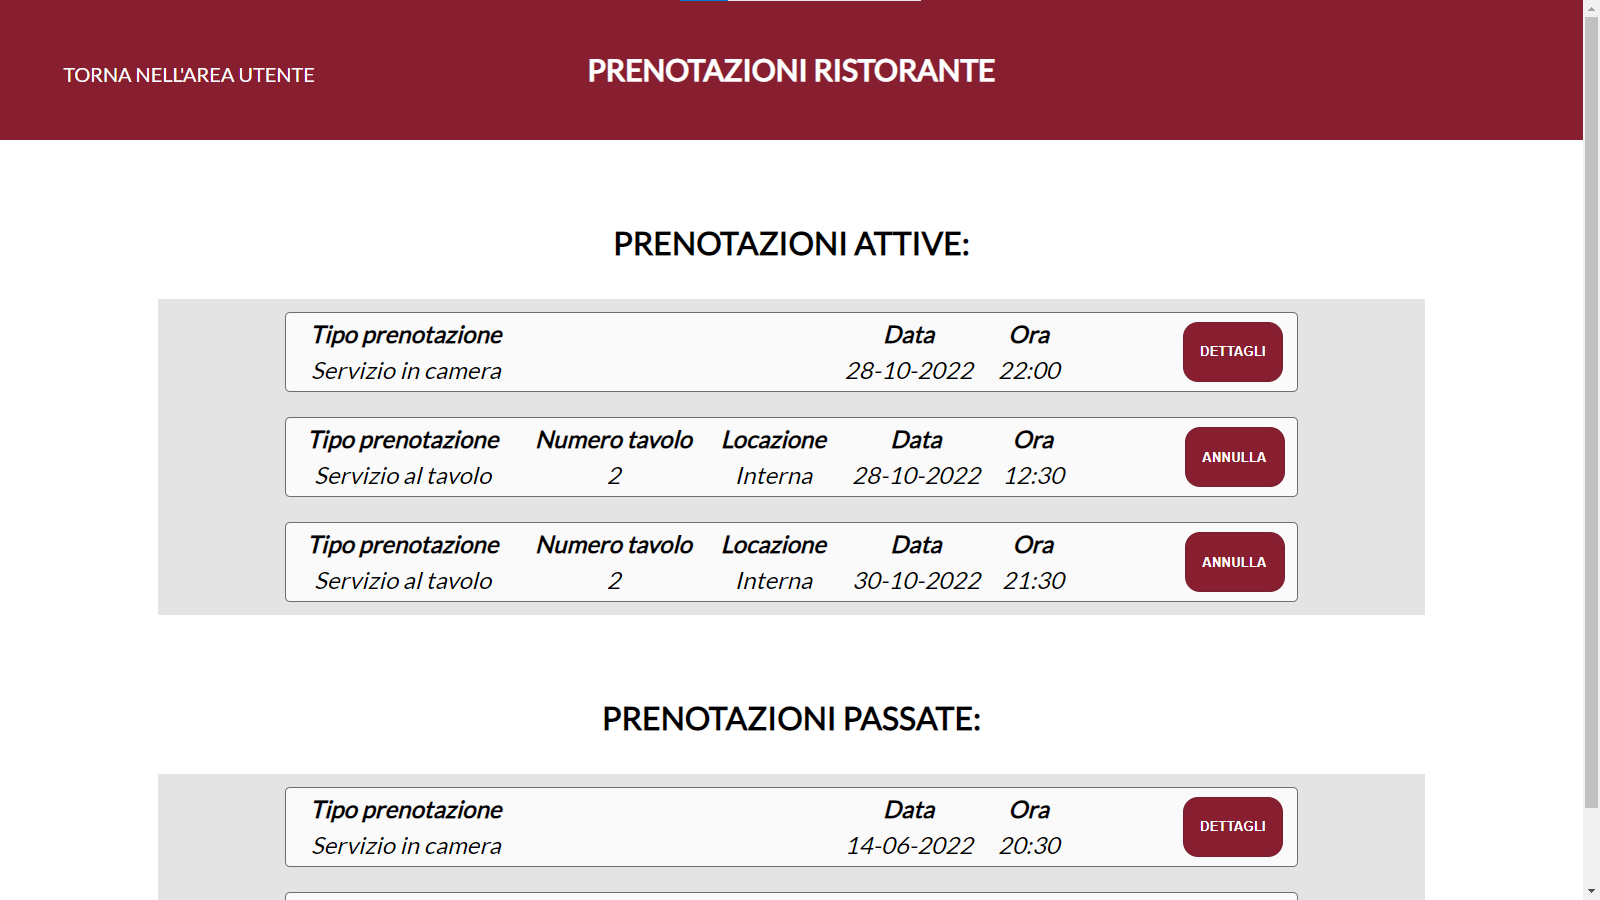
\includegraphics[scale=0.3]{PrenotazioniRistoranteCliente.png}
\caption{Visualizzazione delle prenotazioni del ristorante}
\label{PrenotazioniRistoranteCliente}
\end{figure}

\subsection{Visualizzare il menu}
L'ultimo link accessibile dalla pagina del servizio di ristorazione mostrata in figura \ref{HomepageRistorante} è quello che permette al cliente di visualizzare il menu, figura \ref{MenuCliente}. La pagina ha come unico scopo quello di mostrare in output il menu completo per il servizio in camera. Scontato dire che il menù può presentare delle modifiche derivanti dall'update della concierge (effettuate in uno specifico range orario).
\begin{figure}[!h]
\centering
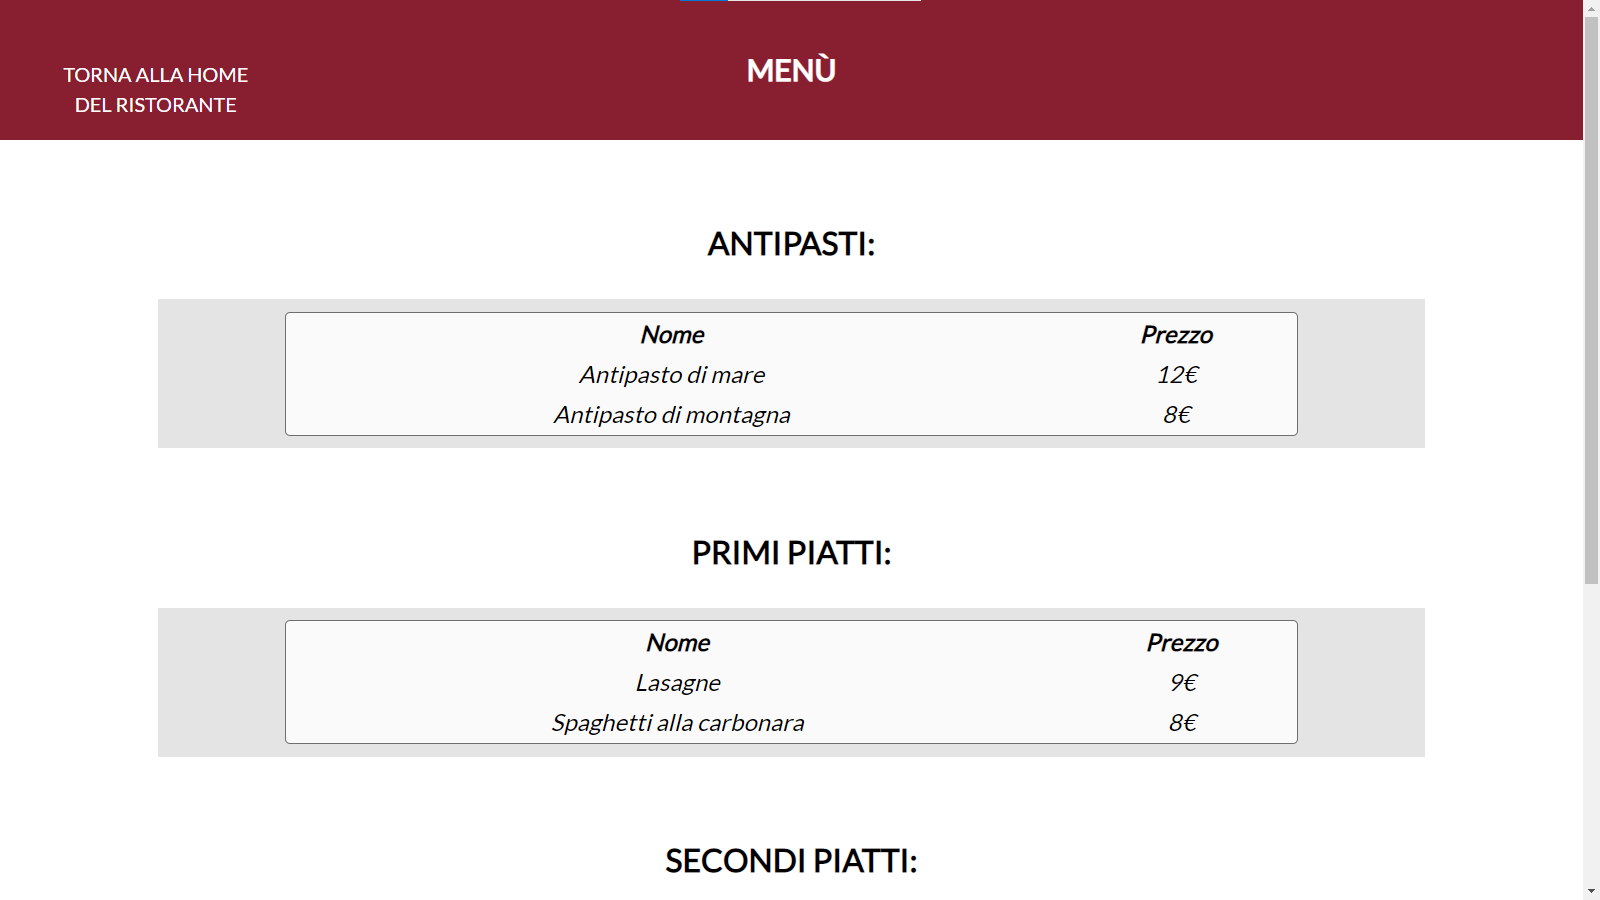
\includegraphics[scale=0.26]{MenuCliente.png}
\caption{Menù del ristorante}
\label{MenuCliente}
\end{figure}


\subsection{Prenotare un'attività}
Tornando nell'area cliente, se il cliente ha intenzione di prenotare un'attività, non deve far altro che interagire con il link denominato \textbf{"ATTIVITÀ"} così da essere indirizzato nella pagina delle attività, come in figura \ref{ListaAttivitaCliente}. 
Qui potrà trovare il solito layout di pagina, due sezioni verticali principali. In quella di sinistra troverà un link per le prenotazioni, in quella di destra invece troverà le informazioni riguardanti le attività presenti nella struttura con l'apposito bottone per prenotarle. Scelta l'attività da prenotare. Il cliente viene portato in una pagina adibita unicamente alla prenotazione di una attività, un esempio è mostrato nella figura \ref{PrenotaAttivita}.\\\\
Qui potrà inserire la \underline{data} (tra quelle presenti nel suo soggiorno approvato), gli \underline{orari di inizio e di fine} (i quali anch'essi sono vincolati da dei range di apertura e di chiusura dell'attività in questione). Qui il cliente può decidere se annullare la prenotazione o proseguire. Presa la seconda strada viene stampato quello che risulta essere il sommario della prenotazione con relativo prezzo totale, figura \ref{ConfermaPrenotazioneAttivita}.\\\\
Qui il cliente ha la possibilità, se ne dispone, di utilizzare dei crediti per poter avere uno sconto sul prezzo finale. Cliccando su conferma, esso si interfaccerà con la pagina di conferma avvenuta prenotazione dell'attività e pochi secondi dopo ritornerà nell'area cliente.
\begin{figure}[!h]
\centering
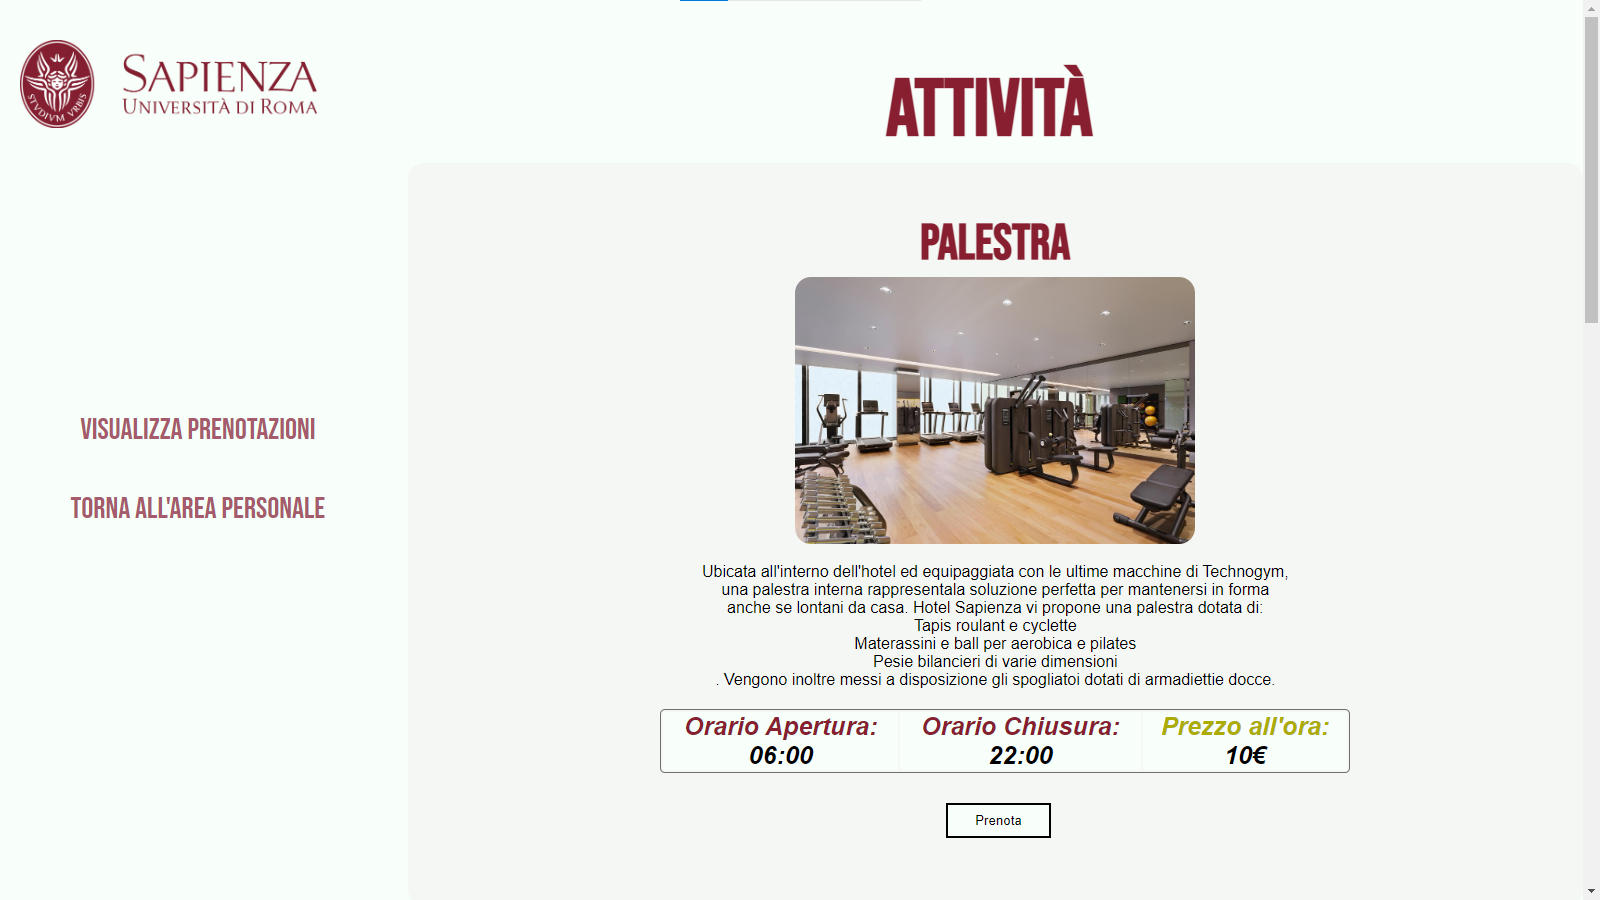
\includegraphics[scale=0.3]{ListaAttivitaCliente.png}
\caption{Lista delle attività dell'hotel}
\label{ListaAttivitaCliente}
\end{figure}\newpage
\begin{figure}[!h]
\centering
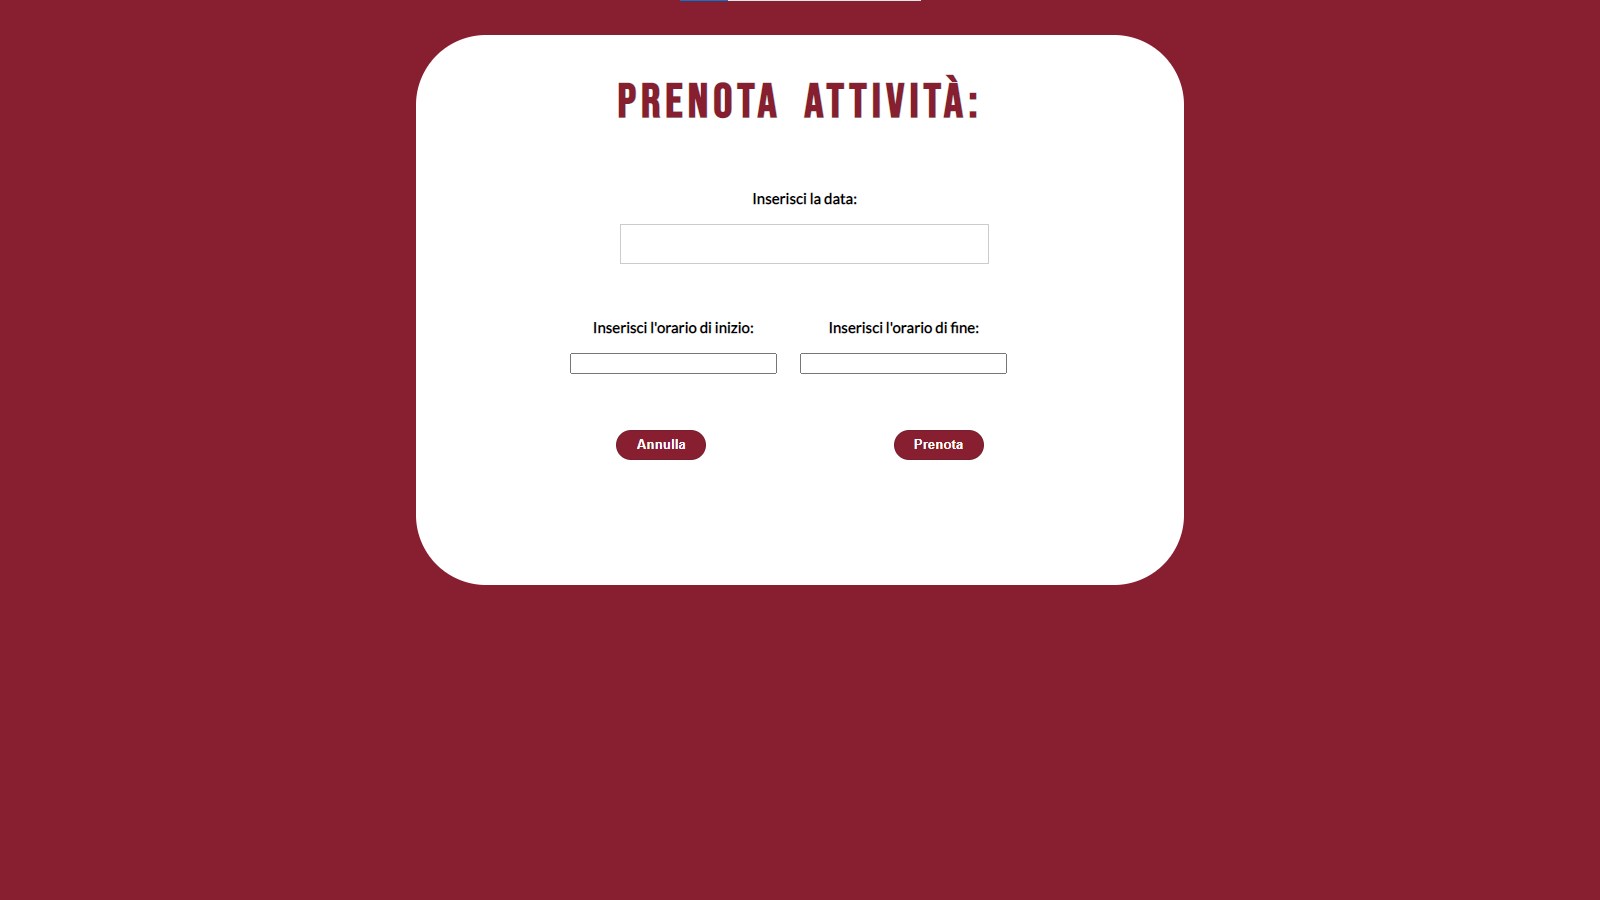
\includegraphics[scale=0.3]{PrenotaAttivita.png}
\caption{Pagina per prenotare un'attività selezionata}
\label{PrenotaAttivita}
\end{figure}
\begin{figure}[!h]
\centering
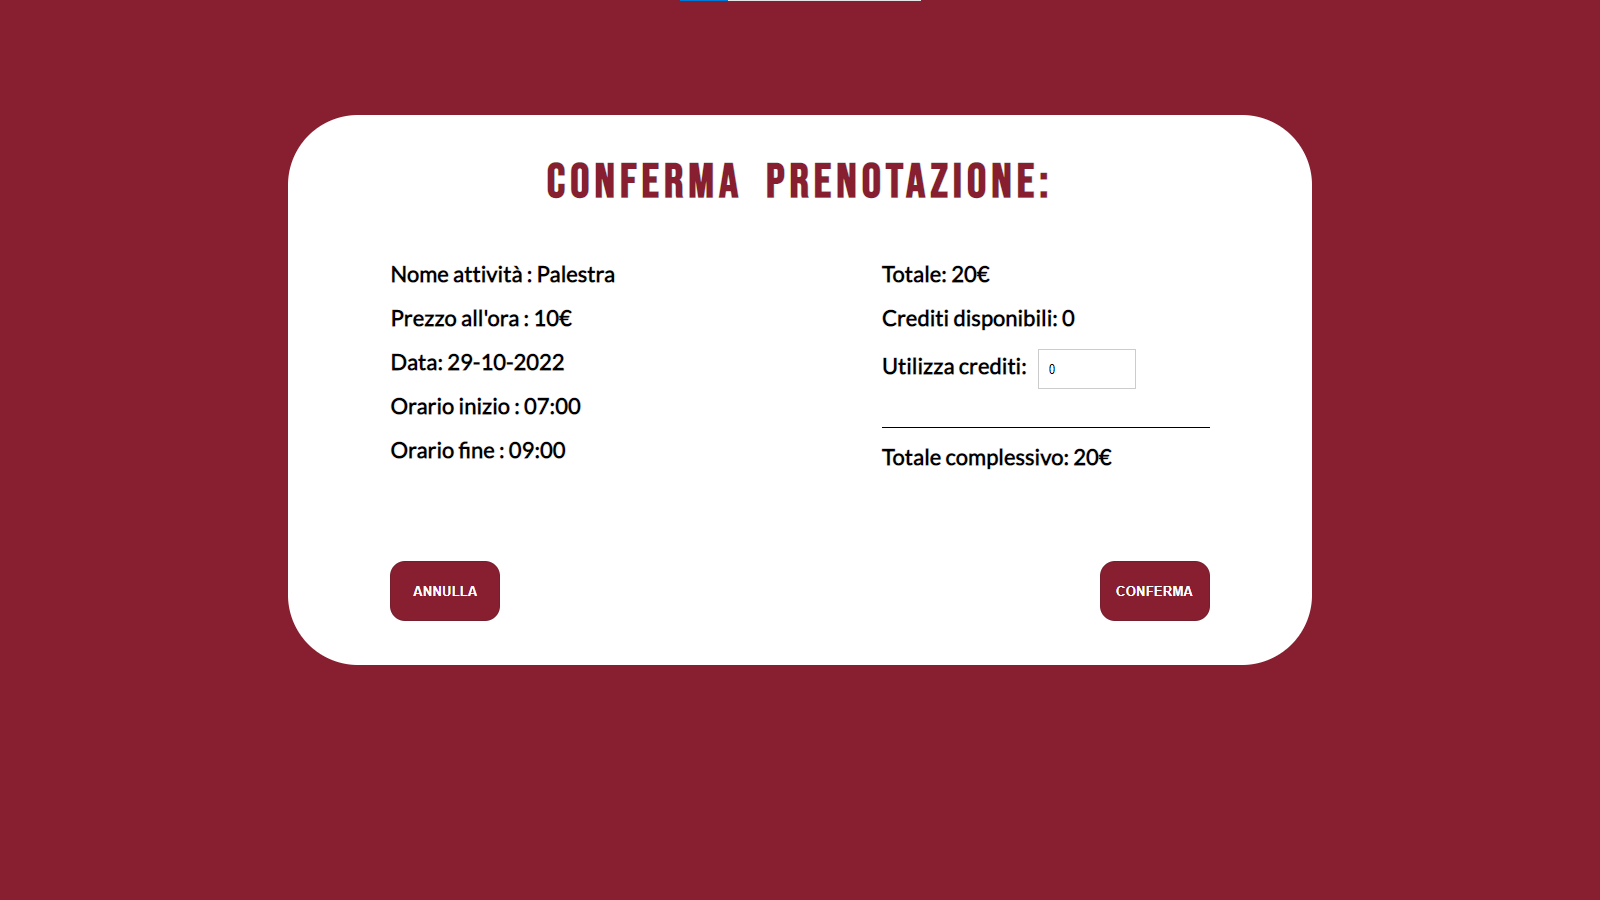
\includegraphics[scale=0.3]{ConfermaPrenotazioneAttivita.png}
\caption{Conferma prenotazione di un'attività}
\label{ConfermaPrenotazioneAttivita}
\end{figure}\newpage

\subsection{Visualizzare le prenotazioni delle attività ed annullarle}
Nella pagina delle attività, ovvero figura \ref{ListaAttivitaCliente}, il cliente può visionare le prenotazioni effettuate cliccando sul link \textbf{"VISUALIZZA PRENOTAZIONI"}. Verrà a lui mostrata una pagina, figura \ref{PrenotazioniAttivitaCliente},  con le sue prenotazioni e tutte le informazioni ad esse associate. Il cliente può decidere di annullarle in qualsiasi momento esso voglia attraverso l'apposito bottone \textbf{"elimina"}. Se si sceglie di eliminare una prenotazione, verrà chiesto al cliente di confermare la propria scelta così da evitare eliminazioni accidentali.
\begin{figure}[!h]
\centering

\includegraphics[scale=0.3]{PrenotazioniAttivitaCliente.png}
\caption{Lista prenotazioni attività}
\label{PrenotazioniAttivitaCliente}
\end{figure}

\subsection{Visualizzare le domande e le relative risposte}
Il cliente, nella propria area utente, può accedere ad un forum privato dell'hotel attraverso il link \textbf{"DOMANDE"} dove tutti i clienti possono scrivere domande e ricevere risposta da altri clienti dell'hotel. La pagina è mostrata in figura \ref{DomandeCliente}. Il cliente avrà anche la possibilità di visualizzare solo le domande di una particolare categoria, andando a scegliere la categoria mediante l'apposito menù a tendina e cliccando il bottone \textbf{conferma}. Il cliente potrà anche visualizzare le proprie domande andando a cliccare sul bottone.  \textbf{visualizza}. Infine, un cliente avrà la possibilità di scegliere una domanda e cliccare sull'apposito bottone \textbf{visualizza risposte} per essere portato nella pagina mostrata in figura \ref{RisposteDomandaCliente} e visualizzare tutte le risposte che sono state inserite nella domanda scelta.\newpage
\begin{figure}[!h]
\centering
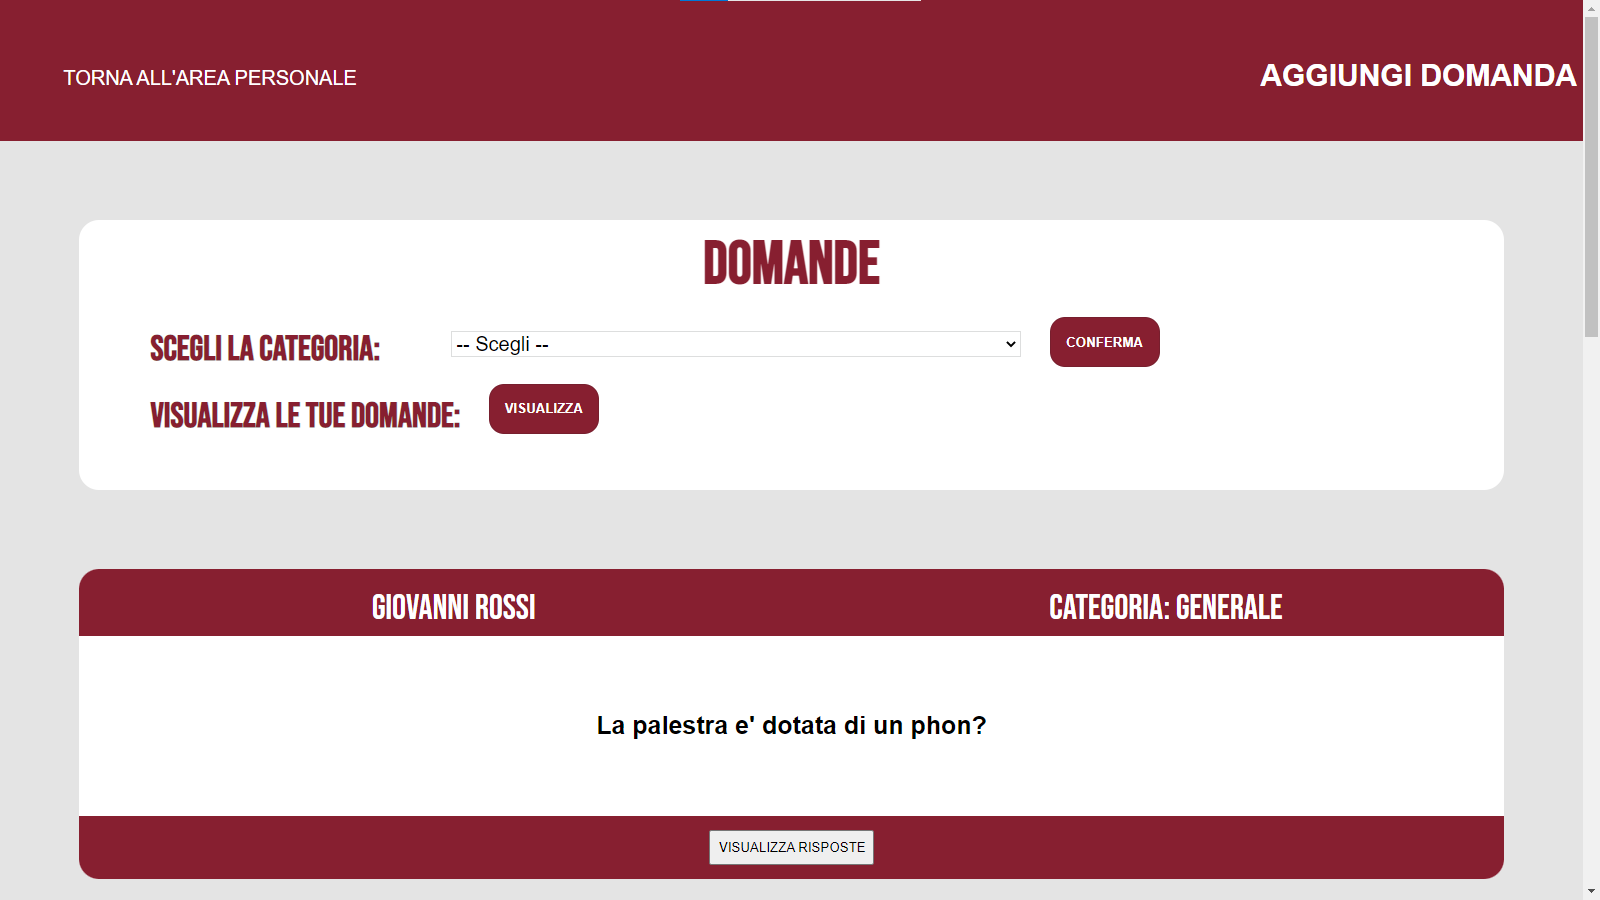
\includegraphics[scale=0.3]{DomandeCliente.png}
\caption{Pagina delle domande dei clienti}
\label{DomandeCliente}
\end{figure}
\begin{figure}[!h]
\centering
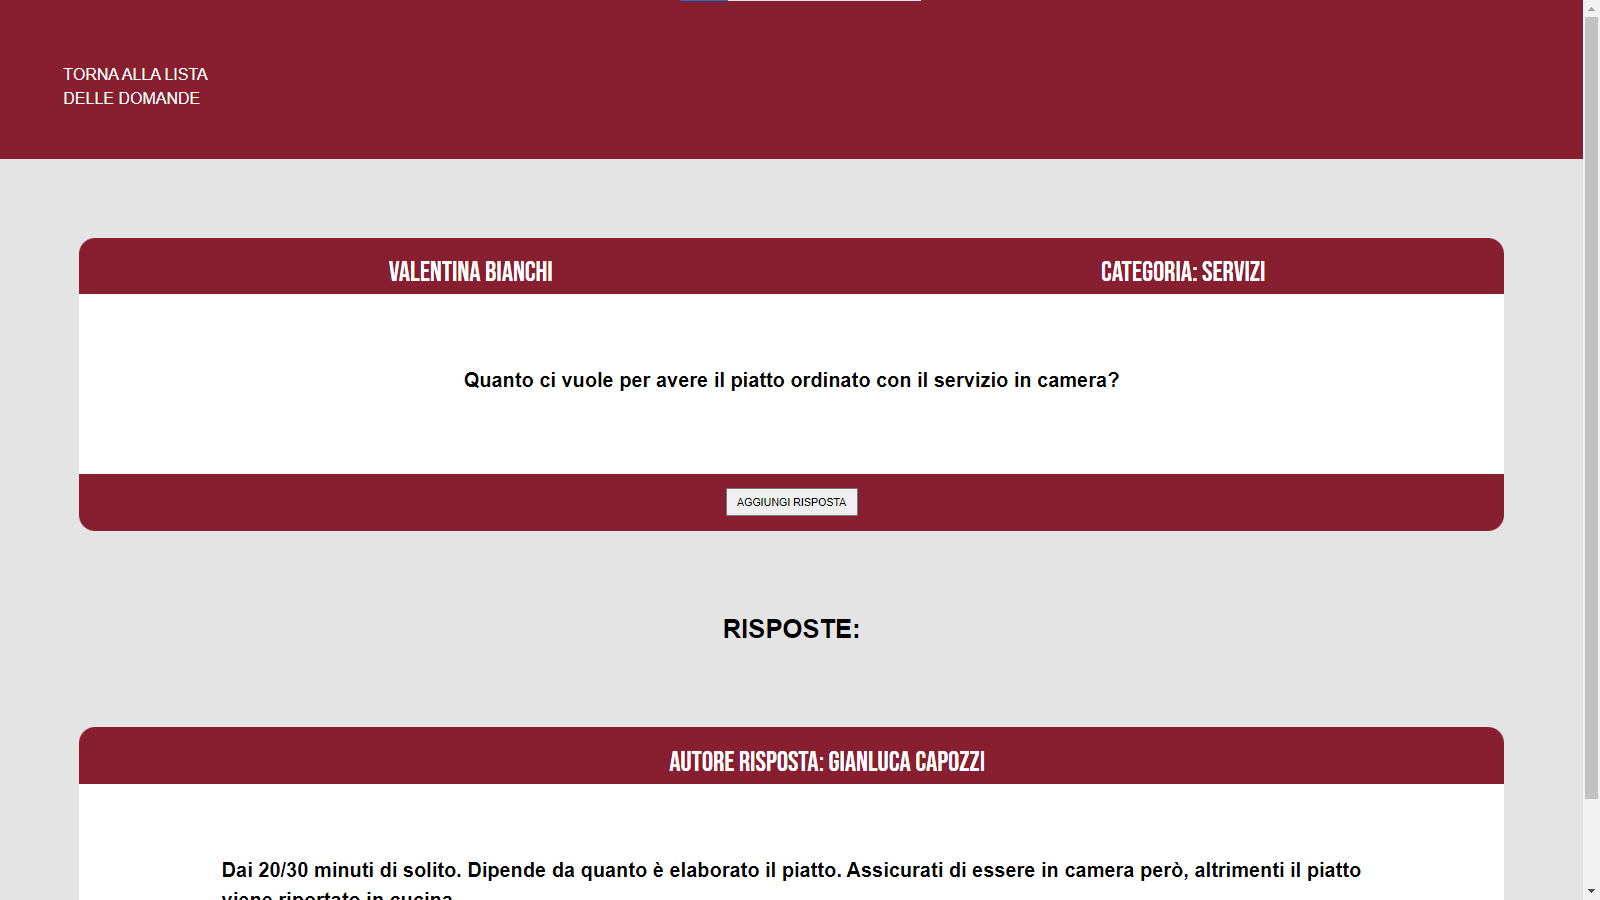
\includegraphics[scale=0.3]{RisposteDomandaCliente.png}
\caption{Lista delle risposte di una domanda}
\label{RisposteDomandaCliente}
\end{figure}

\subsection{Aggiungere una domanda}
Per aggiungere una domanda nella pagina delle domande, il cliente non deve far altro che cliccare sulla scritta \textbf{"AGGIUNGI DOMANDA"} in alto a destra, mostrato nella figura \ref{DomandeCliente}, attraverso la quale verrà portato nella pagina mostrata in figura \ref{AggiungiDomanda} , dove dovrà poi scegliere la categoria della domanda ed inserire il testo di quest'ultima.
\begin{figure}[!h]
\centering
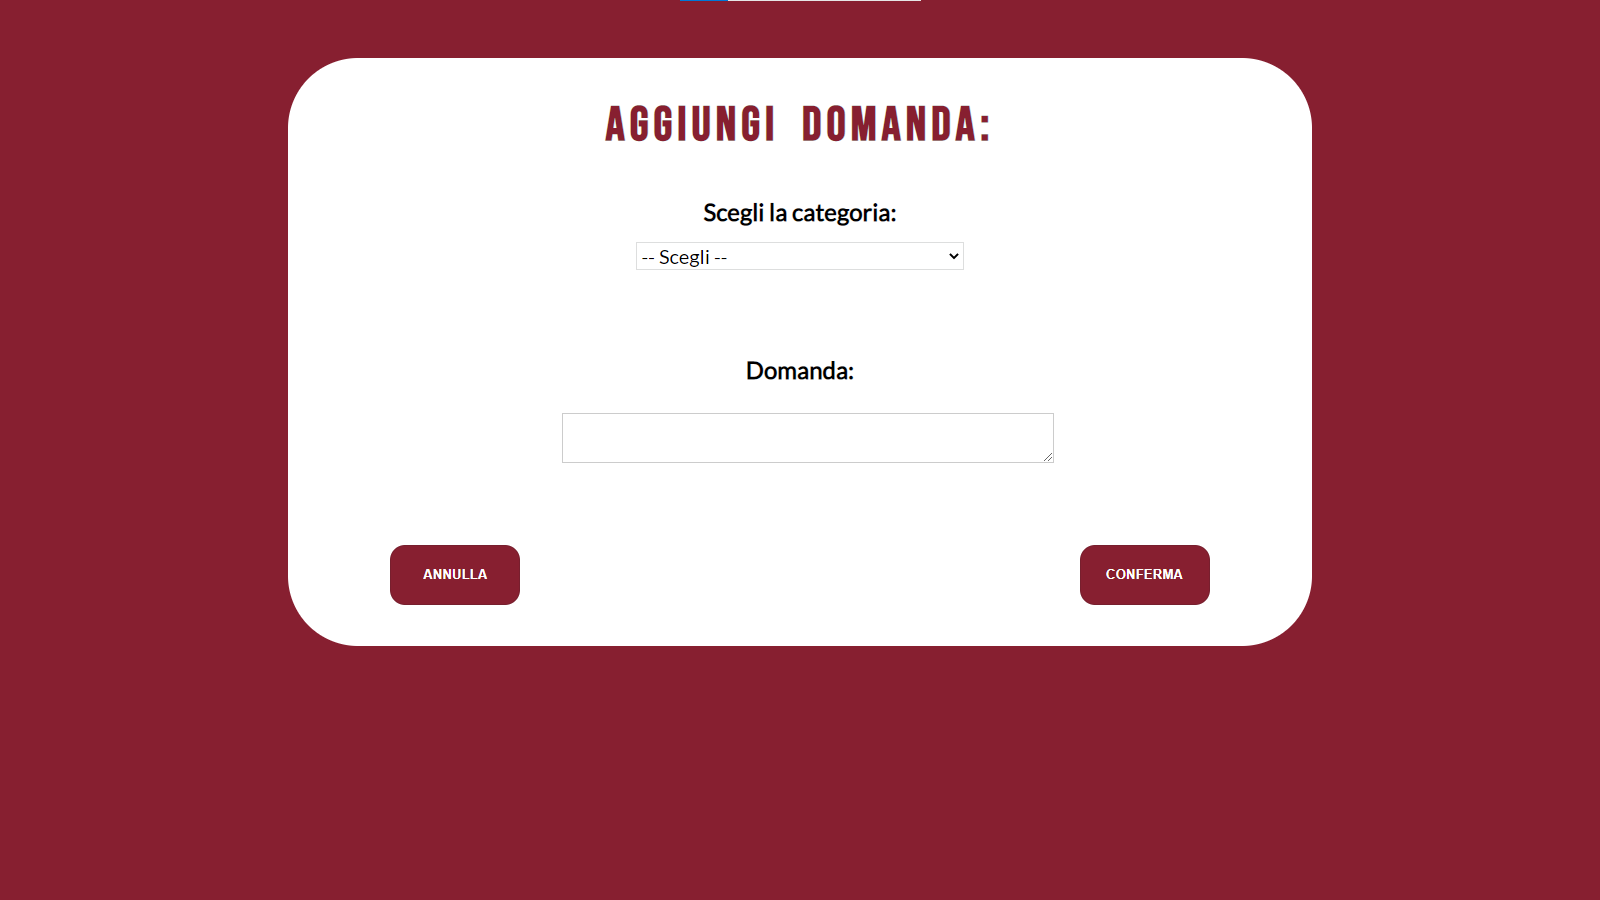
\includegraphics[scale=0.3]{AggiungiDomanda.png}
\caption{Aggiunta di una domanda}
\label{AggiungiDomanda}
\end{figure}

\subsection{Rispondere ad una domanda}
Il cliente può rispondere ad una domanda cliccando sul bottone \textbf{"aggiungi risposta"} della domanda a cui vuole rispondere, mostrato in figura \ref{RisposteDomandaCliente}. Il cliente può rispondere solamente nel caso in cui la categoria della domanda gli appartiene, ovvero abbia avuto un qualche tipo di esperienza in quel settore.

\subsection{Aggiungere una recensione}
Il cliente nella pagina delle recensioni, se autentificato, vedrà comparire in alto a destra della pagina la scritta \textbf{"AGGIUNGI RECENSIONE"}, come mostrato nella figura \ref{RecensioniCliente}. Cliccandoci, egli verrà portato nella pagina mostrata in figura \ref{AggiungiRecensione}. Il cliente avrà l'opportunità di scrivere una recensione su una categoria specifica (di cui deve necessariamente aver fatto già esperienza), potendo inserire anche una valutazione espressa da una a cinque stelle. Una volta svolta la recensione, essa potrà essere giudicata dagli altri utenti in base all'utilità e al possibile comune accordo. Il cliente autore della recensione riceverà dei crediti in base alla somma di questi giudizi.\newpage
\begin{figure}[!h]
\centering
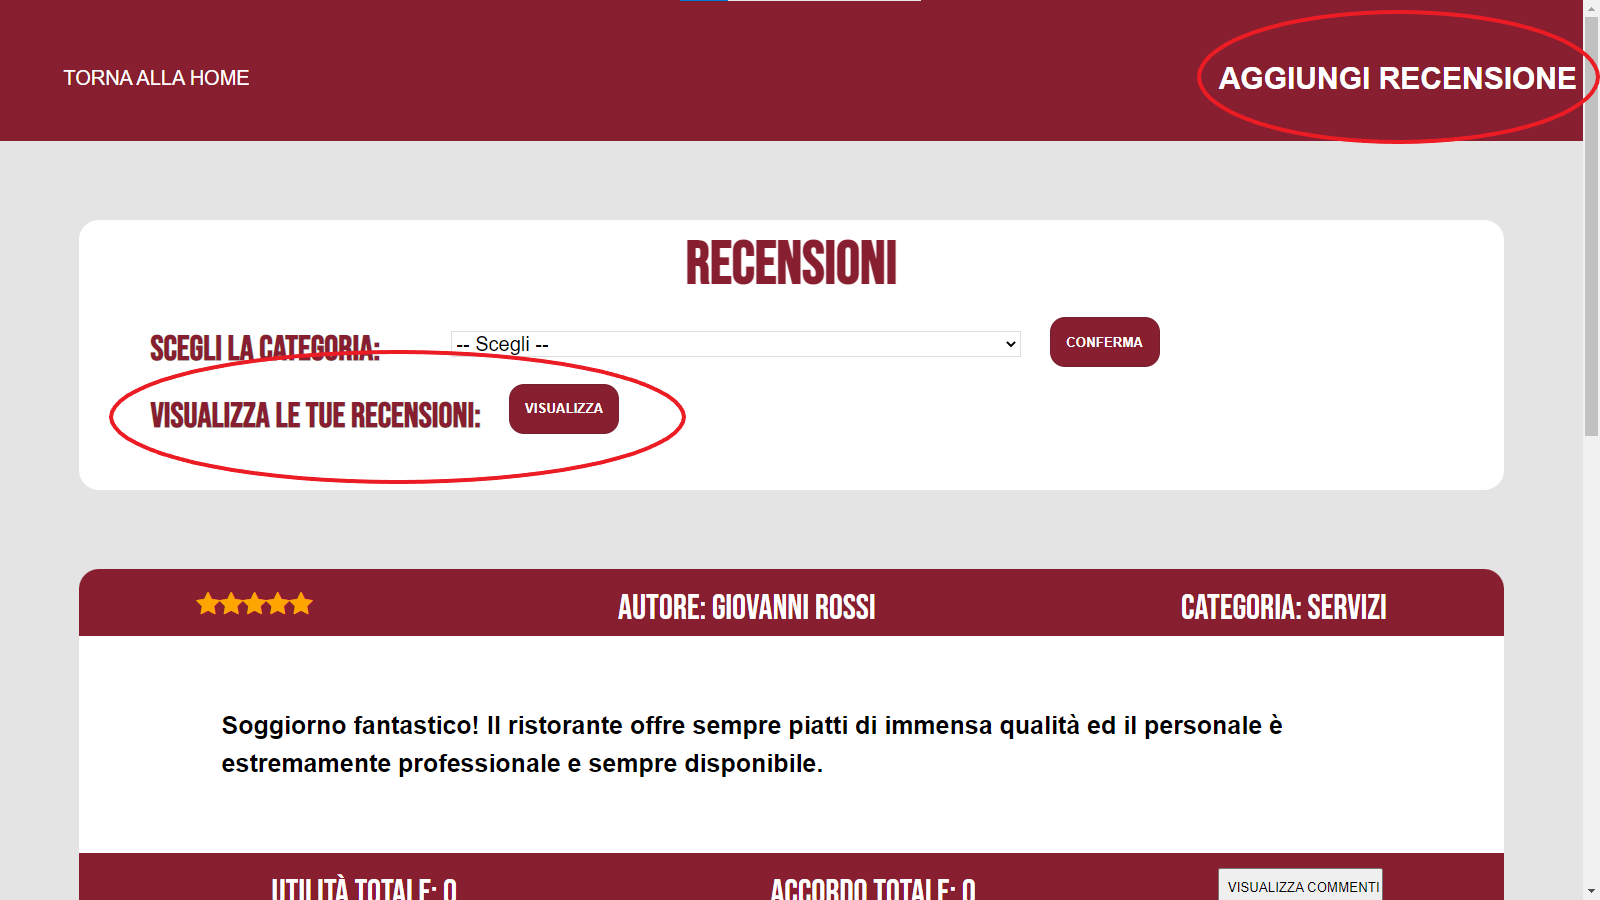
\includegraphics[scale=0.3]{RecensioniCliente.png}
\caption{Pagina delle recensioni - cliente}
\label{RecensioniCliente}
\end{figure}

\begin{figure}[!h]
\centering
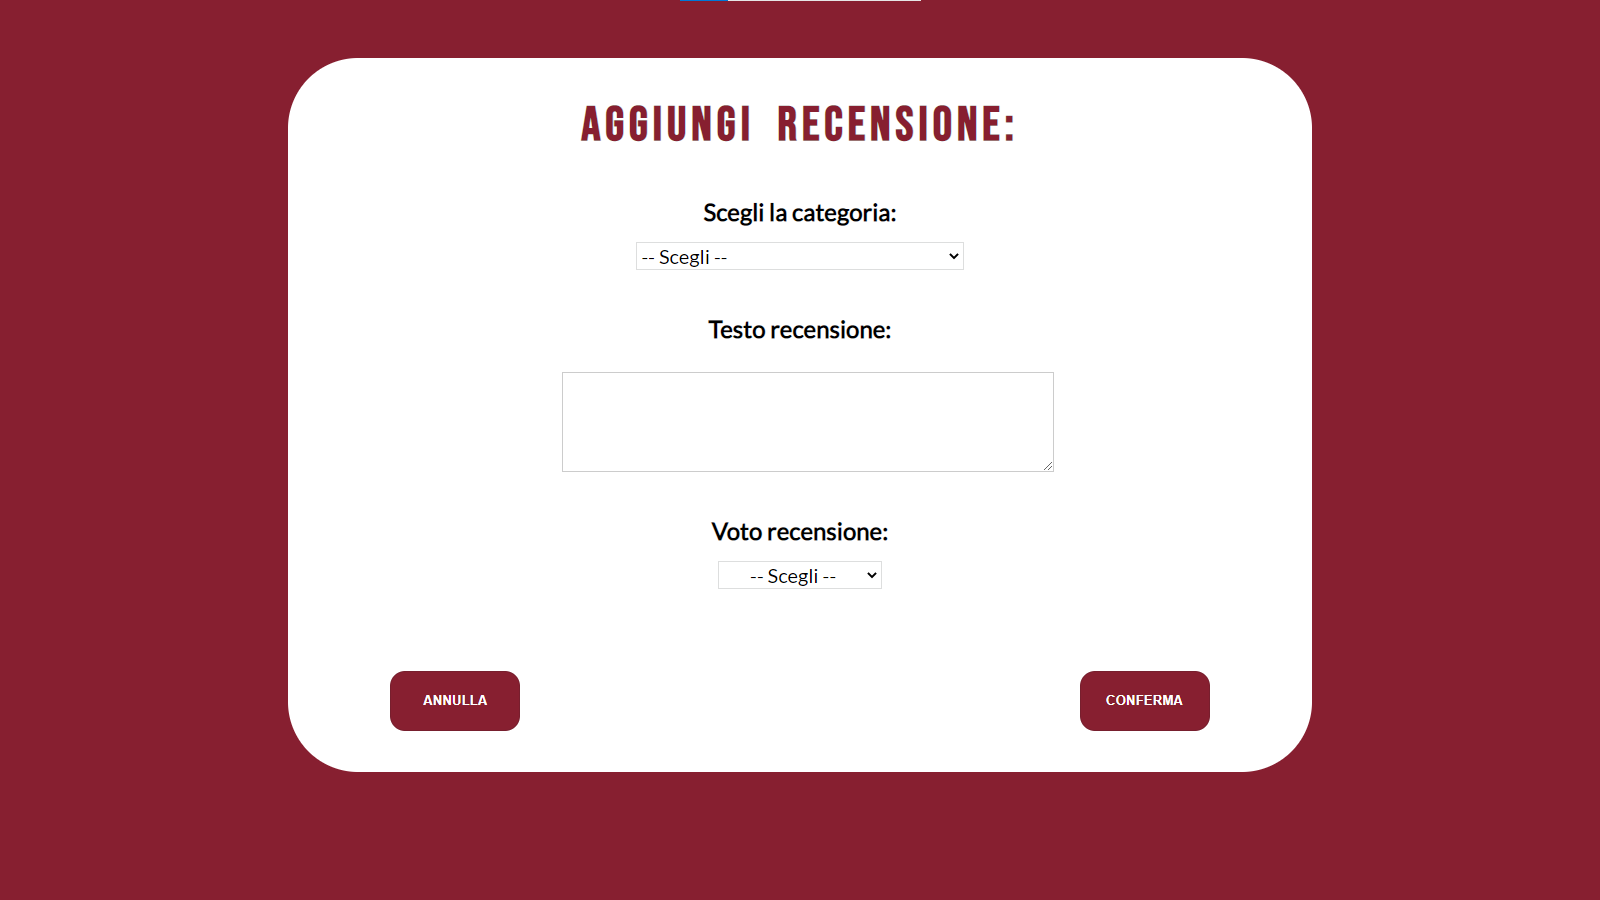
\includegraphics[scale=0.3]{AggiungiRecensione.png}
\caption{Aggiunta di una recensione}
\label{AggiungiRecensione}
\end{figure}

\subsection{Rispondere ad una recensione o ad un commento}
Il cliente può rispondere ad una recensione o al commento di una recensione per esprimere il suo parere in relazione al contenuto della medesima o del medesimo. Nel farlo anch'esso potrà poi essere giudicato con gli stessi criteri di una recensione, come descritto nella sottosezione precedente, così da ricevere anch'esso dei crediti in merito. 

\subsection{Giudicare una recensione/un commento/una risposta al commento}
Per giudicare una recensione, un commento o una risposta ad un commento il cliente non deve far altro che cliccare sul bottone \textbf{"inserisci giudizio"}. Una volta fatto, sarà portato ad inserire due valori in una apposita pagina, figura \ref{InserisciGiudizio}. Il primo che va a testimoniare l'utilità della recensione/commento/risposta con un valore che va da zero a cinque, e il secondo che esprime quanto il cliente sia d'accordo con la recensione/commento/risposta dell'altro cliente, con un valore adesso che oscilla tra zero e tre. Una volta inserito, sarà anche in grado di modificarlo con un apposito bottone \textbf{"modifica giudizio"} che ora prende il posto del precedente. 
\begin{figure}[!h]
\centering
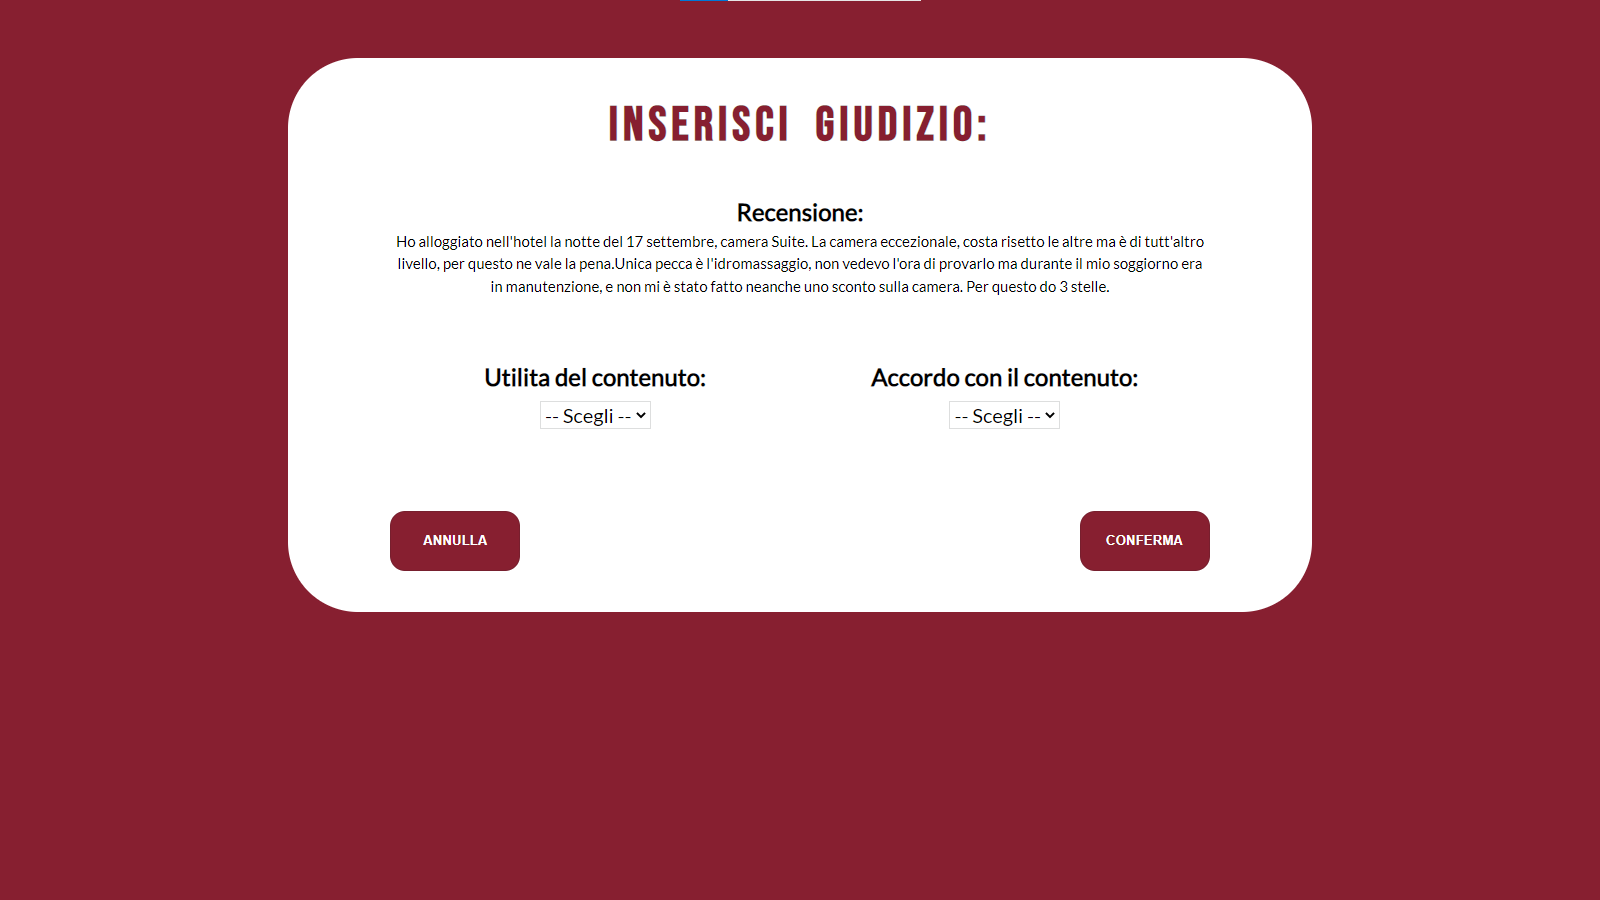
\includegraphics[scale=0.3]{InserisciGiudizio.png}
\caption{Inserimento di un giudizio}
\label{InserisciGiudizio}
\end{figure}

\subsection{Visualizzare i propri dati e modificarli}
Nell'area cliente mostrata in figura \ref{AreaCliente} troviamo il link per i dati personali, una pagina dove il cliente potrà prendere visione dei propri dati personali, compresi i crediti disponibili e la somma dei giudizi ricevuti. Sempre in questa pagina potrà modificare un suo qualsiasi dato personale cliccando sul bottone di fianco al dato da modificare. Un esempio è mostrato nella figura \ref{DatiPersonali}. Nella figura \ref{ModificaDatiPersonali} c'è un esempio di un cliente che intende modificare il proprio indirizzo civico. Scendendo nella pagina mostrata nella figura \ref{DatiPersonali} il cliente avrà la possibilità di visualizzare le informazioni relative al proprio soggiorno attivo (se presente) e le informazioni su tutti i soggiorni passati del cliente o con pagamento rifiutato.
\begin{figure}[!h]
\centering
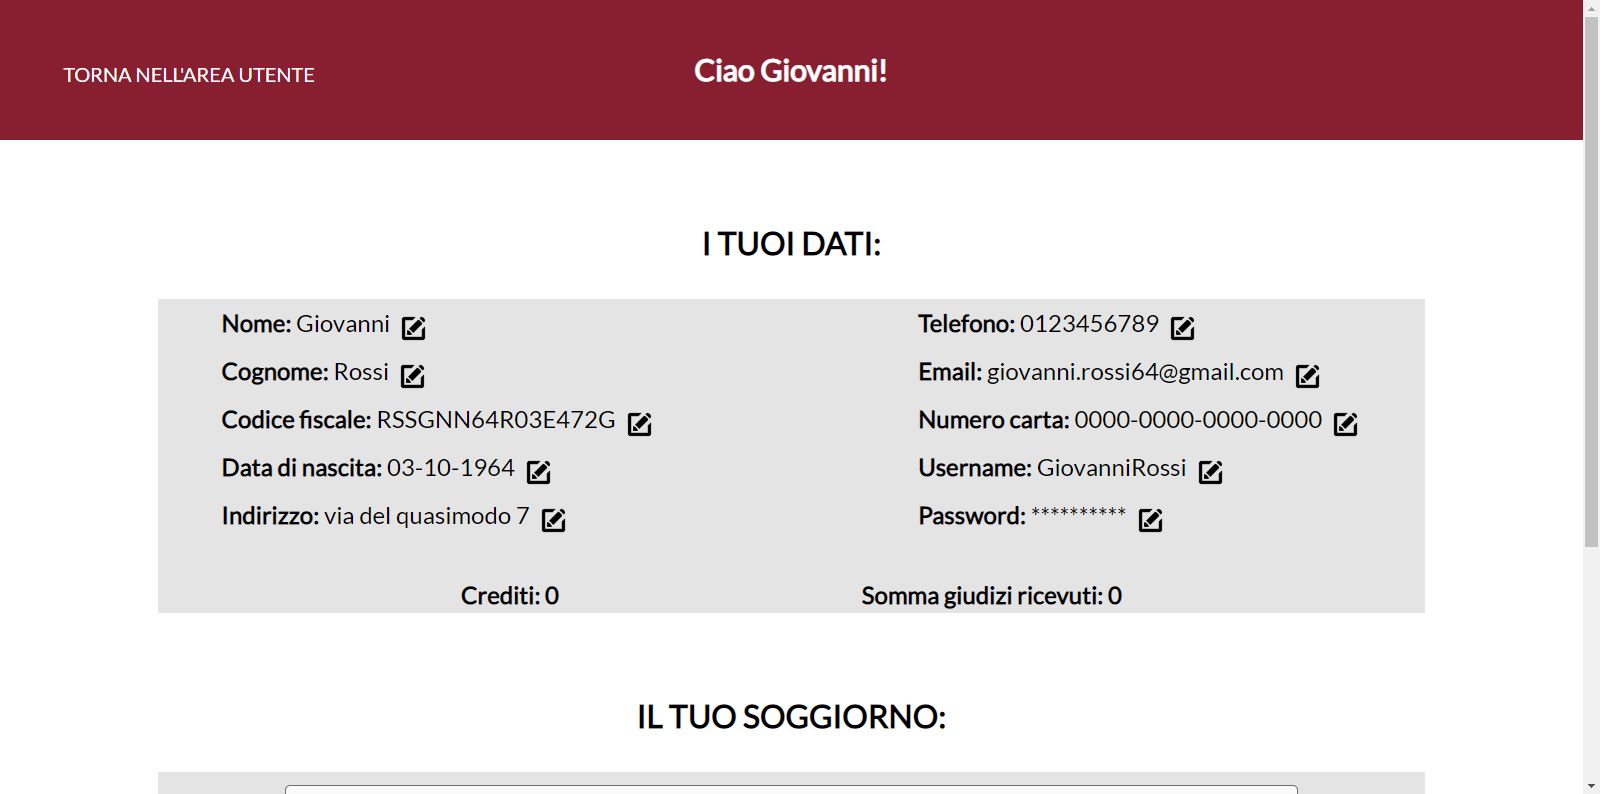
\includegraphics[scale=0.3]{DatiPersonali.png}
\caption{Dati personali di un cliente}
\label{DatiPersonali}
\end{figure}

\begin{figure}[!h]
\centering
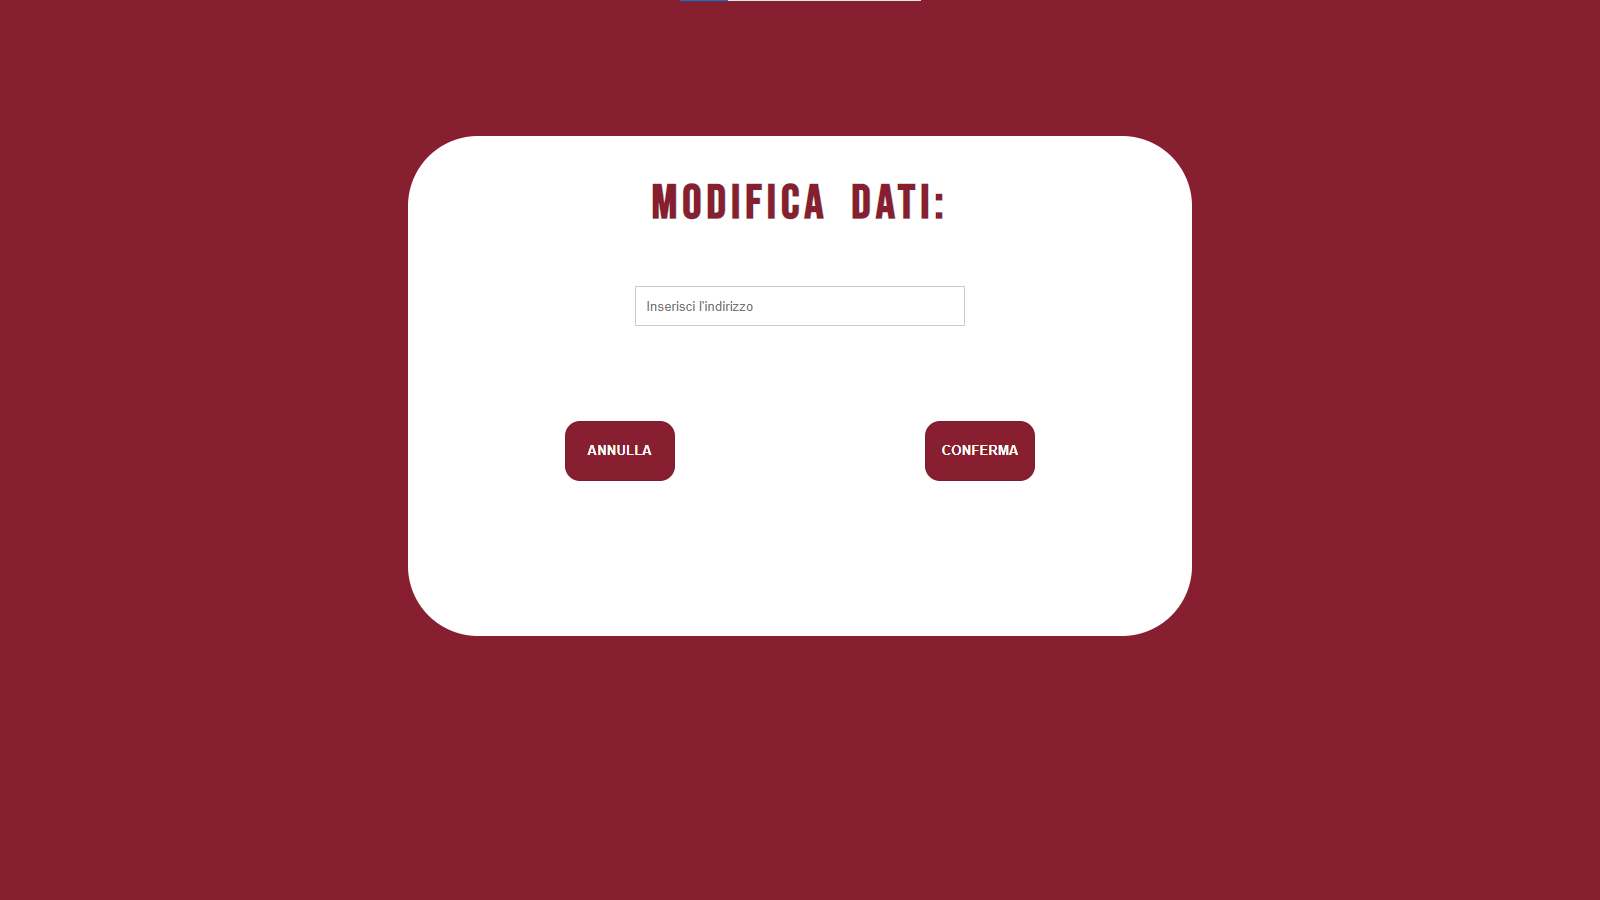
\includegraphics[scale=0.3]{ModificaDatiPersonali.png}
\caption{Modifica dei dati personali}
\label{ModificaDatiPersonali}
\end{figure}

\section{Concierge}
In questa sezione andiamo ad analizzare tutte le funzionalità usufruibili dal tipo di utenza \textbf{"Concierge"}.\\\\
Assumiamo che l'utente visitatore si sia autenticato come \textbf{Concierge} attraverso la pagina di login. Dopo aver fatto l'accesso, la schermata iniziale sarà quella dell'area della concierge, come mostrato nella figura \ref{AreaConcierge}. \\\\
La pagina presenta due sezioni verticali, quella di sinistra, sezione di principale interesse, dove sono presenti dei link, quella di destra composta da un titolo che ci informa dell'area in cui ci troviamo con relativa immagine sottostante presente solo a scopo decorativo. Andremo ora ad analizzare in dettaglio le varie funzionalità della concierge con i relativi link associati. Ovviamente tra questa funzionalità sono comprese tutte quelle dell'utente visitatore, ad accezione di quella di registrazione (sottosezione 2.1.6) e quella di prenotazione di un soggiorno (sottosezione 2.1.4).
\begin{figure}[!h]
\centering

\includegraphics[scale=0.3]{AreaConcierge.png}
\caption{Area personale della concierge}
\label{AreaConcierge}
\end{figure}

\subsection{Modifica del menù del ristorante}
La prima funzionalità che andremo ad esaminare è quella della modifica del menù. La concierge, infatti, interagendo con il link \textbf{"MODIFICA MENÙ RISTORANTE"} verrà indirizzata nella pagina per la visualizzazione del menù. Se dovesse accedere a questa pagina in un orario diverso da quello prestabilito dall'admin per l'update del menù, allora essa sarà in grado solamente di visualizzarlo, e verrà stampata a schermo una scritta di avviso con il range orario appena citato. La pagina in questione con la modifica abilitata è mostrata nella figura \ref{MenuStaff}.
\begin{figure}[!h]
\centering
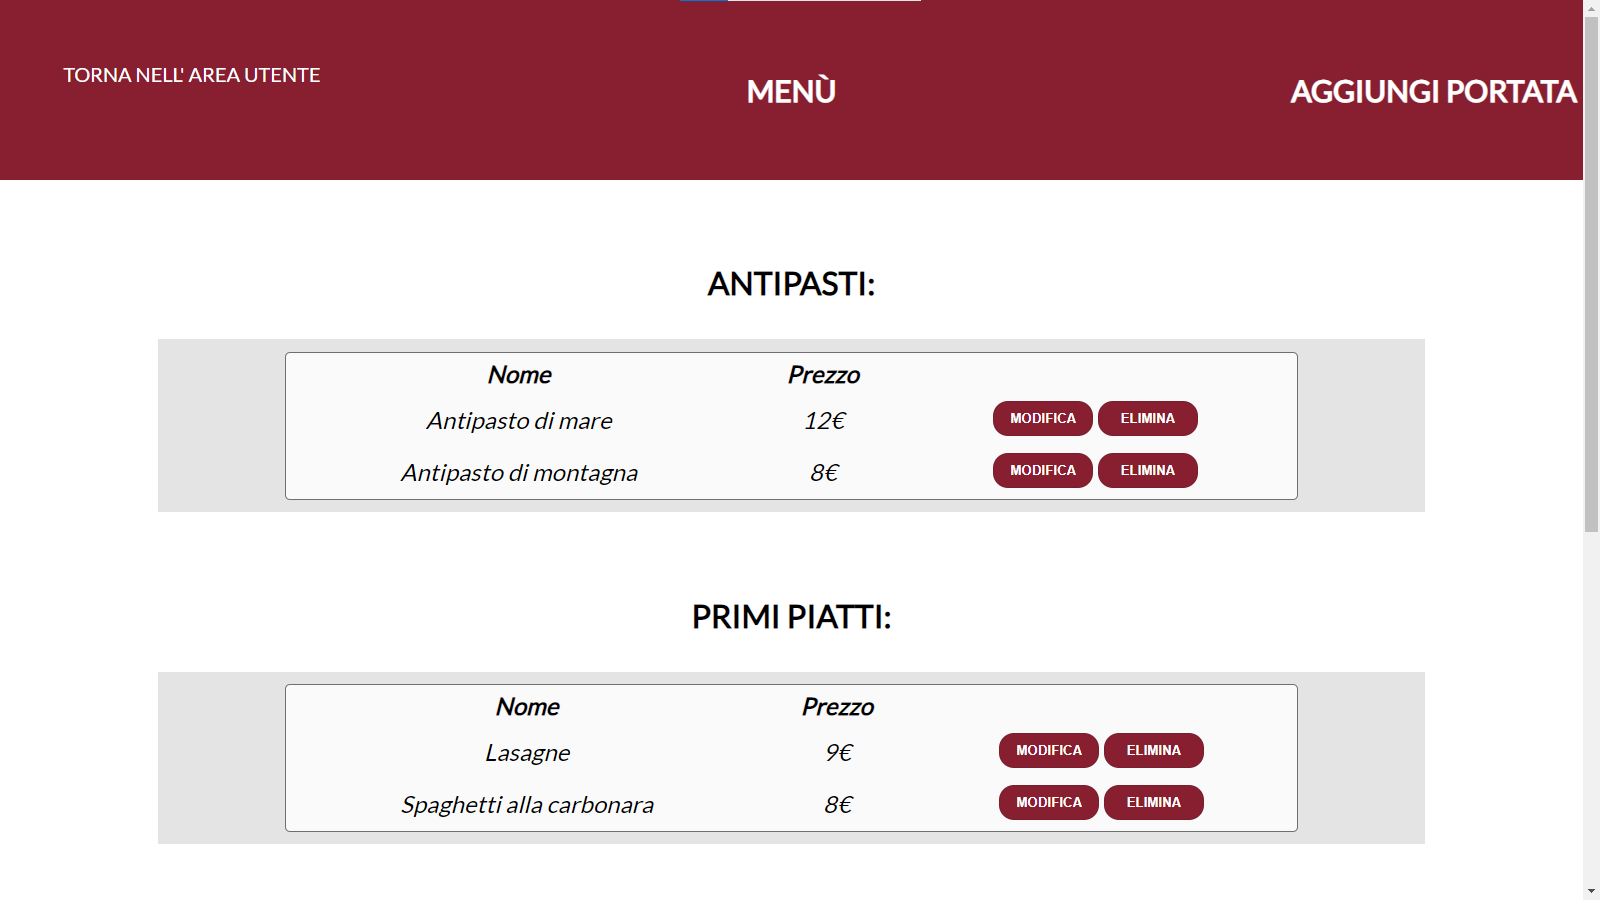
\includegraphics[scale=0.3]{MenuStaff.png}
\caption{Visualizzazione del menù per modificarlo}
\label{MenuStaff}
\end{figure}\\
Al di fianco di ogni portata vengono mostrati dei bottoni per poterla \textbf{rimuovere} o \textbf{modificarla} e una scritta \textbf{"AGGIUNGI PORTATA"}, nella parte superiore destra della pagina, in caso voglia aggiungere una portata al menù.\\\\
In caso di rimozione di una portata, verrà chiesto all'utente una conferma, per evitare errori accidentali. Per la modifica invece verrà chiesto di inserire o un nuovo nome (il quale deve essere differente da quelli già presenti nel menù), o un nuovo prezzo. Esempio mostrato nella figura \ref{ModificaPortata}.\\\\
Nel caso di aggiunta, gli verrà chiesto di inserire il nome della portata, la tipologia della portata (le opzioni possibili sono: antipasto, primo, secondo e dolce) e il prezzo associato. Esempio mostrato nella figura \ref{AggiungiPortata}.\newpage

\begin{figure}[!h]
\centering
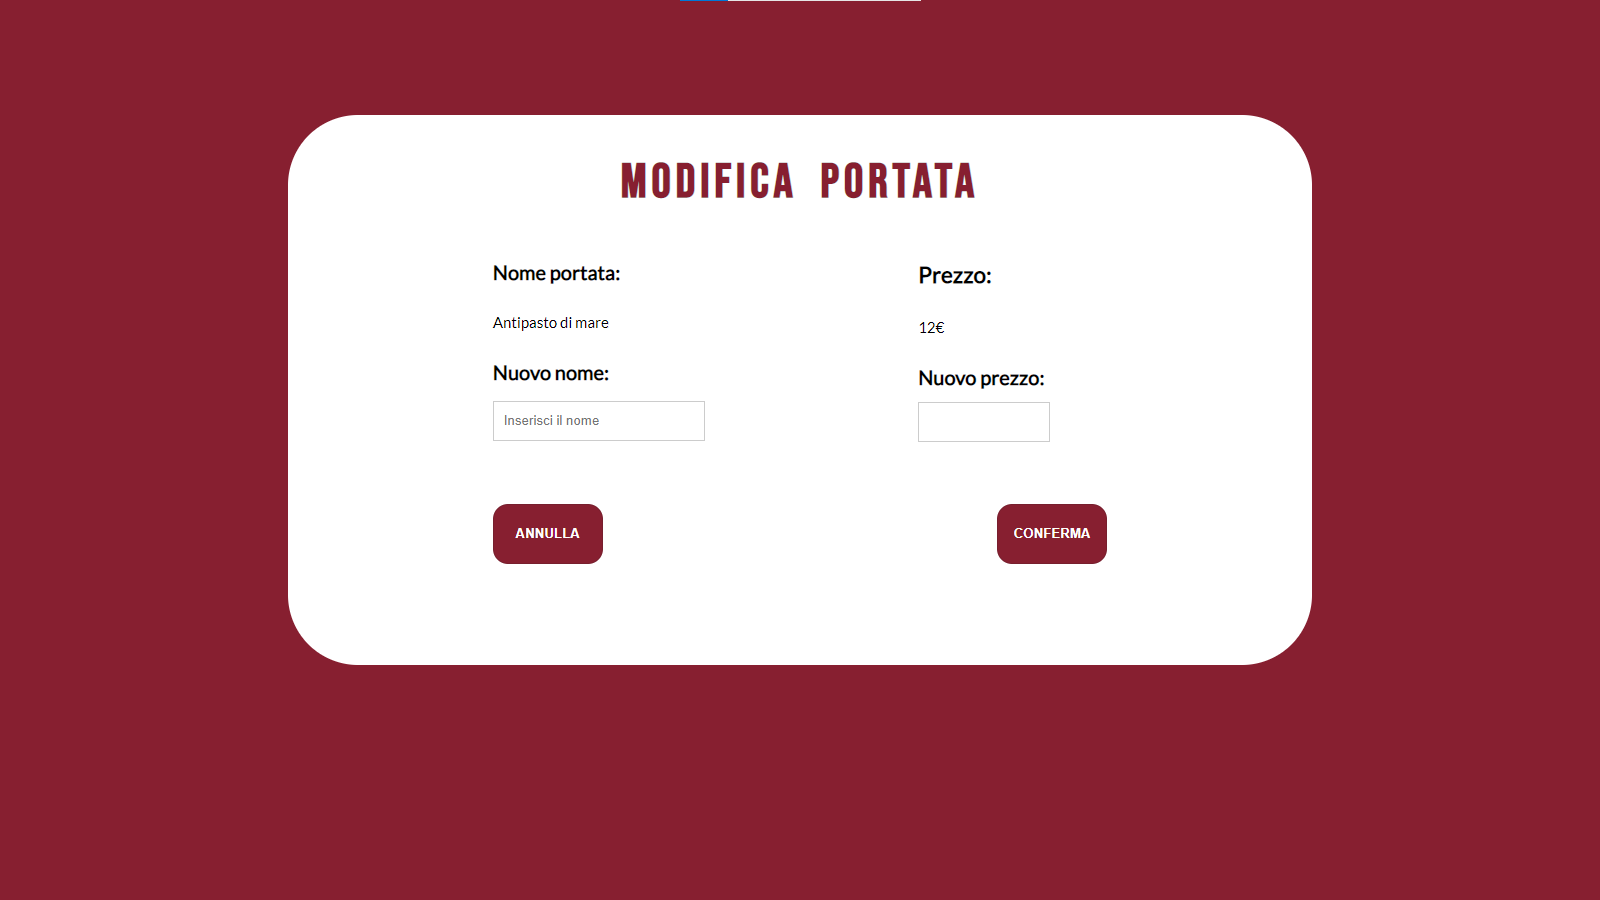
\includegraphics[scale=0.3]{ModificaPortata.png}
\caption{Modifica di una portata}
\label{ModificaPortata}
\end{figure}

\begin{figure}[!h]
\centering
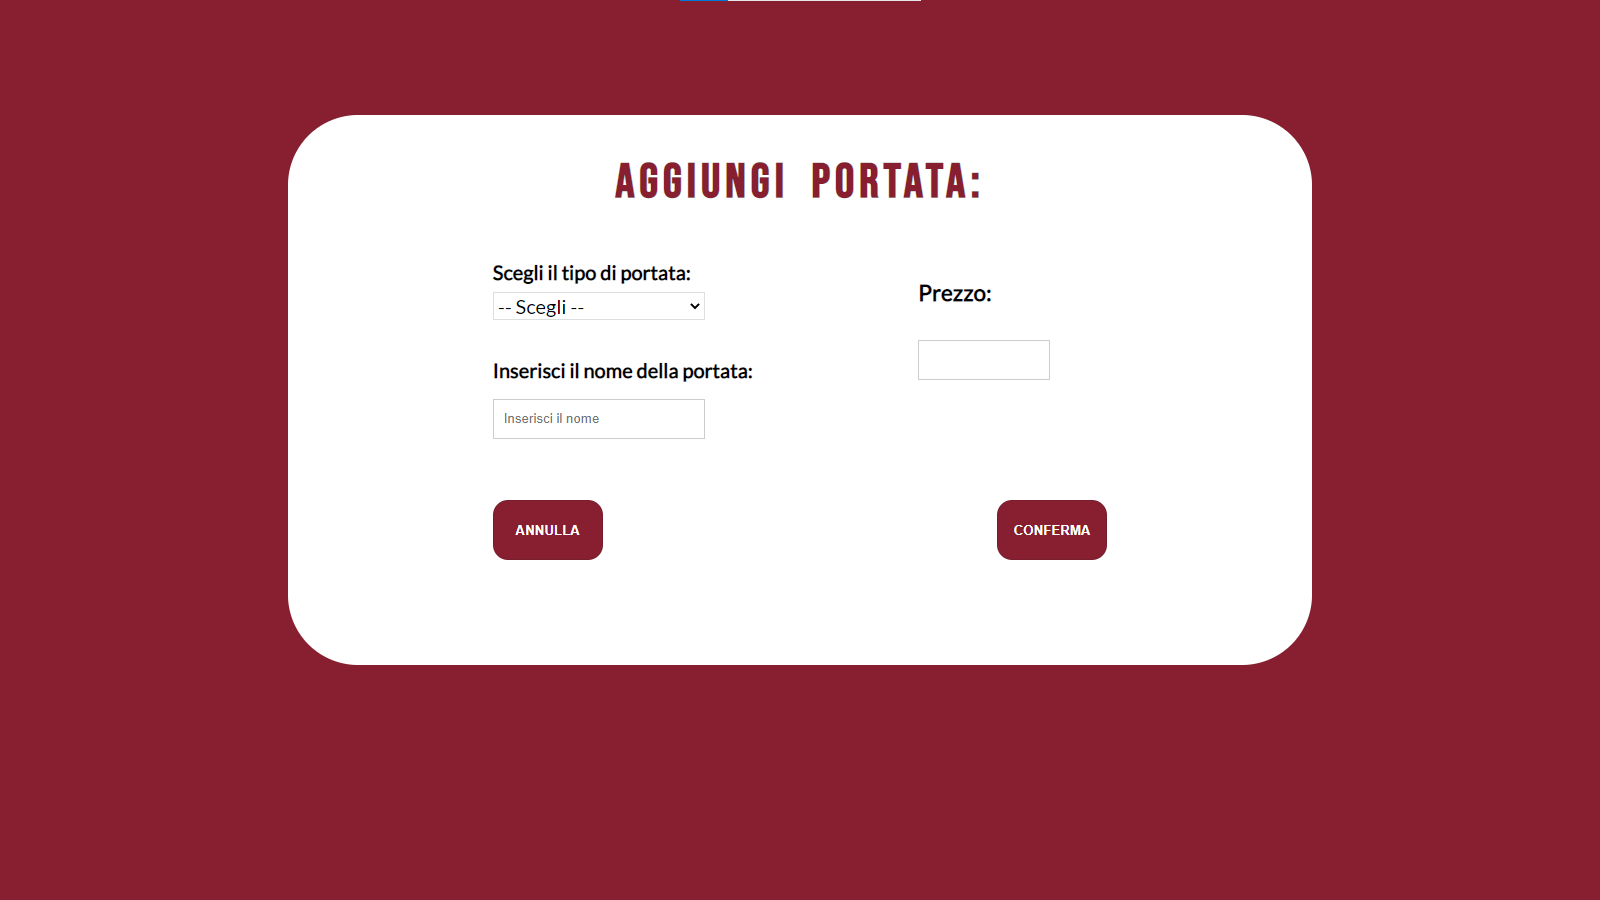
\includegraphics[scale=0.3]{AggiungiPortata.png}
\caption{Aggiunta di una portata}
\label{AggiungiPortata}
\end{figure}

\subsection{Modifica degli orari delle attività e del ristorante}
La concierge è in grado di poter modificare gli orari di apertura e di chiusura, di una determinata attività e di pranzo e di cena del ristorante, attraverso l'interazione con il link \textbf{"MODIFICA ORARI"} presente nella propria area utente.\\\\
Una volta fatto, l'utente potrà decidere, nella pagina raffigurata nella figura \ref{ListaOrari}, se modificare gli orari del ristorante o dell'attività.\\\\ 
Nel caso decidesse di intraprendere la prima strada, allora gli sarà permesso di cambiare gli orari sia di apertura che di chiusura del ristorante. Esempio mostrato nella figura \ref{ModificaOrariRistorante}.\\\\
Per quanto riguarda la seconda, gli sarà data la possibilità di decidere gli orari di apertura e di chiusura dell'attività selezionata nella pagina. Esempio mostrato nella figura \ref{ModificaOrariAttivita}.

\begin{figure}[!h]
\centering
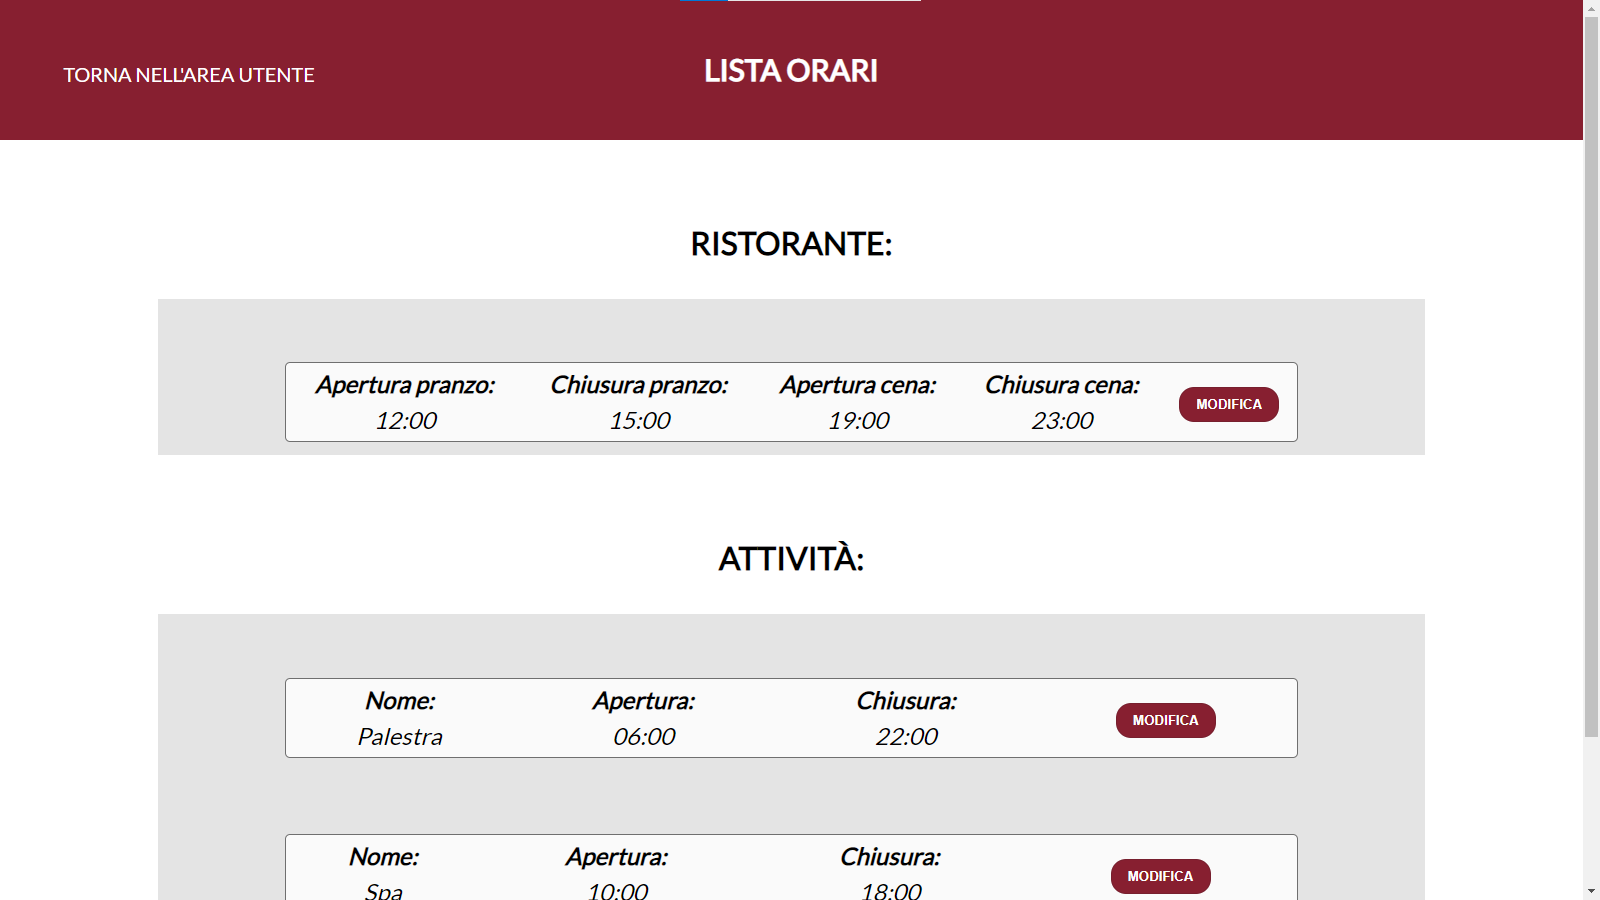
\includegraphics[scale=0.22]{ListaOrari.png}
\caption{Lista degli orari delle attività e del ristorante}
\label{ListaOrari}
\end{figure}

\begin{figure}[!h]
\centering
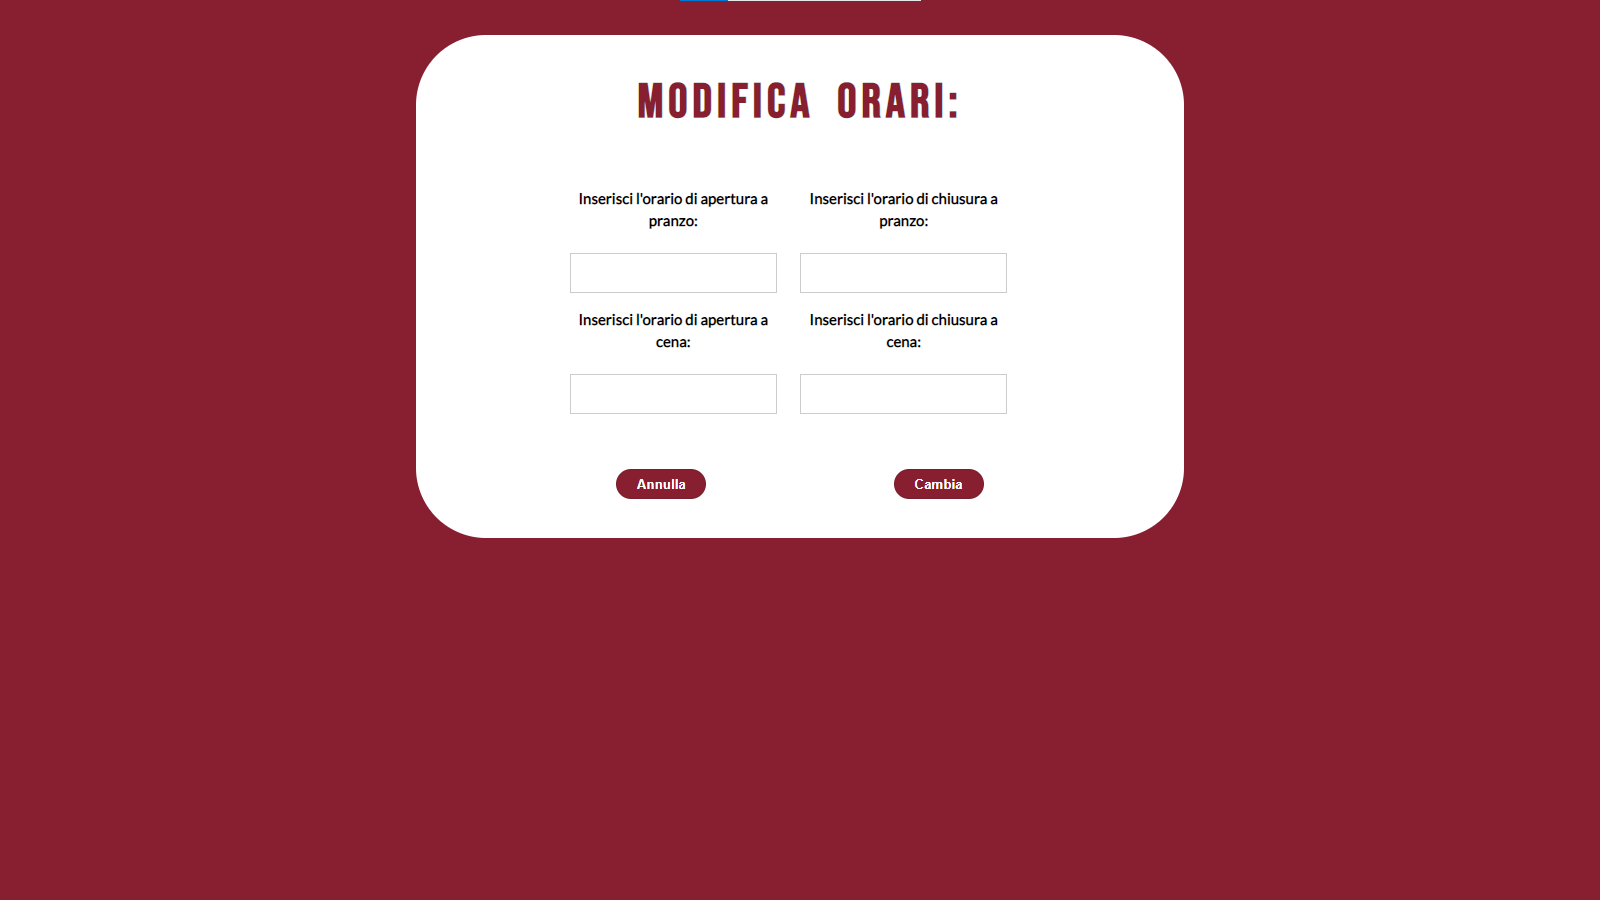
\includegraphics[scale=0.23]{ModificaOrariRistorante.png}
\caption{Modifica degli orari del ristorante}
\label{ModificaOrariRistorante}
\end{figure}\newpage

\begin{figure}[!h]
\centering
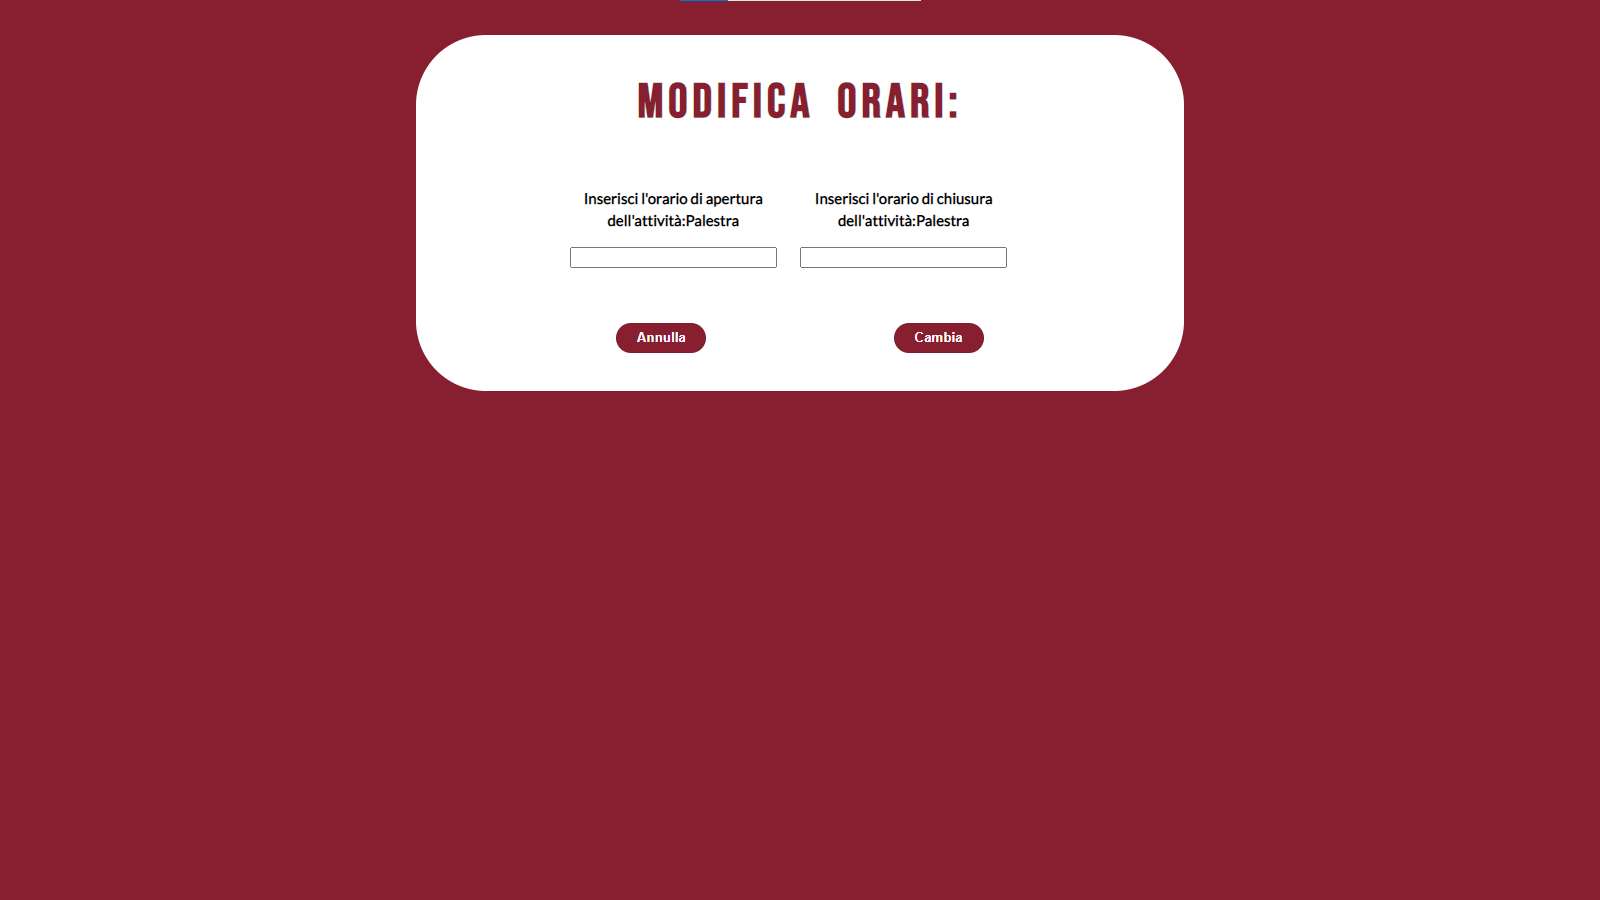
\includegraphics[scale=0.3]{ModificaOrariAttivita.png}
\caption{Modifica degli orari del ristorante}
\label{ModificaOrariAttivita}
\end{figure}

\subsection{Modifica delle attività}
Ulteriore funzione che possiede la concierge è quella di poter modificare i dati relativi ad una attività specifica presente all'interno della struttura. Cliccando sul link \textbf{"ATTIVITÀ"} presente nell'area utente verranno mostrate, in una pagina differente mostrata in figura \ref{ListaAttivitaStaff}, una lista di attività con un bottone \textbf{"modifica"} associato ad ognuna di esse. Dopo aver scelto l'attività da modificare, la concierge potrà decidere quale dato modificare tra il \underline{nome}, il \underline{link dell'immagine}, la \underline{descrizione} e il \underline{prezzo orario} dell'attività. Può anche decidere di cambiare solo alcuni tra questi dati, i campi dei dati lasciati vuoti non verranno alterati. Esempio mostrato nella figura \ref{ModificaAttivita}. Se sono gli orari che si vogliono cambiare, troverà anche un link attraverso il quale potrà interfacciarsi con la pagina adibita alla modifica degli orari come spiegato nella sottosezione 2.3.2.\pagebreak
\begin{figure}[!h]
\centering
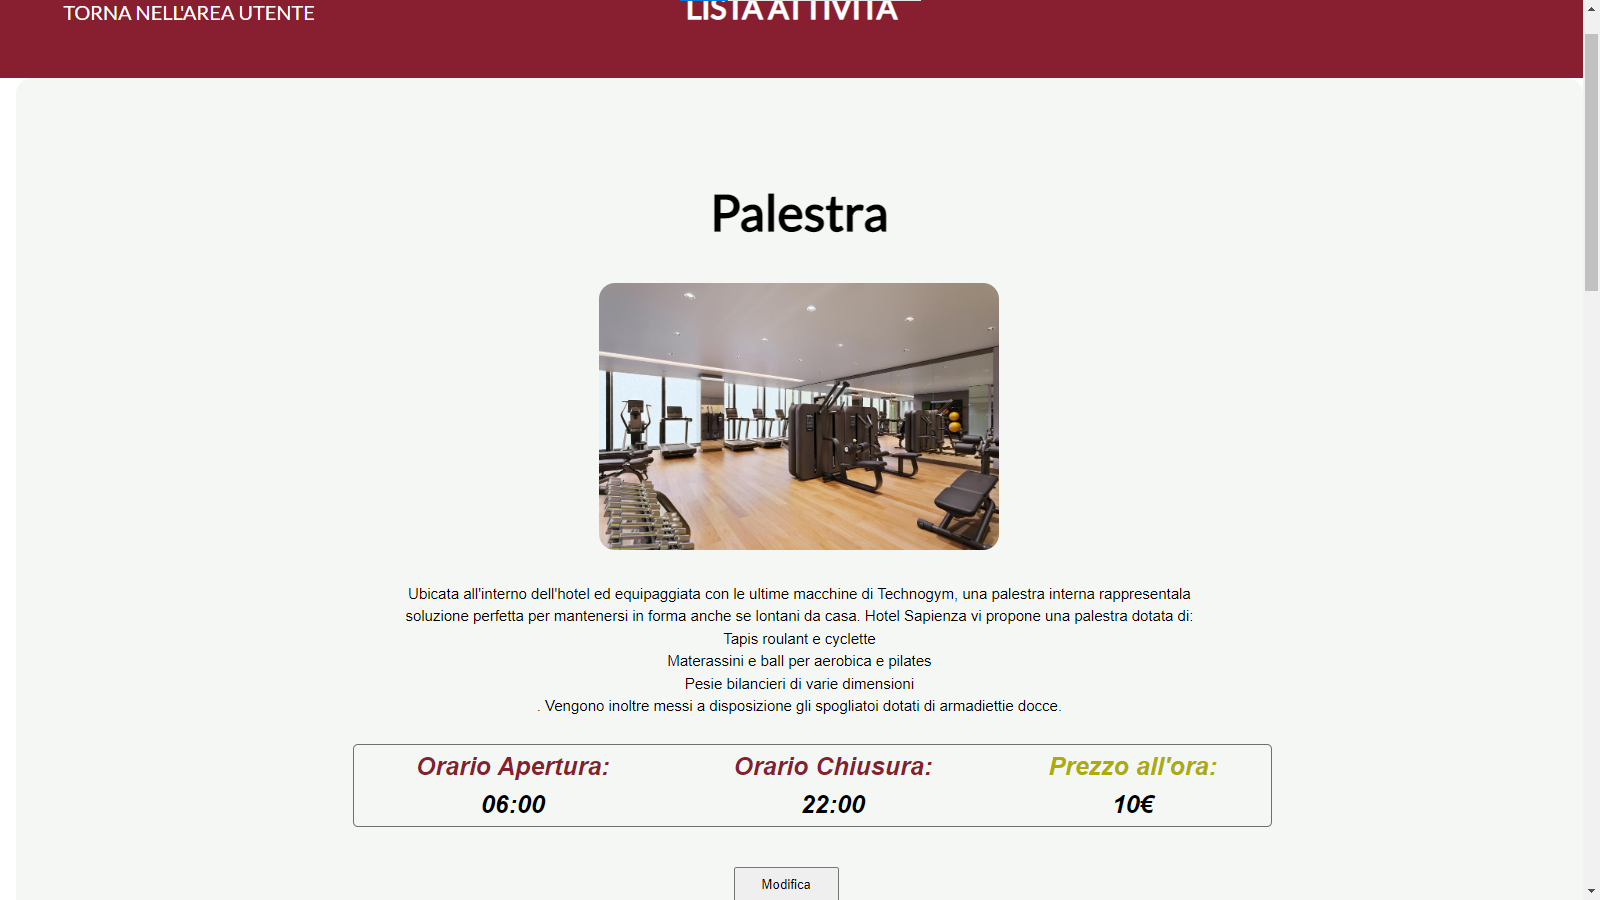
\includegraphics[scale=0.3]{ListaAttivitaStaff.png}
\caption{Lista delle attività per poterle modificare}
\label{ListaAttivitaStaff}
\end{figure}

\begin{figure}[!h]
\centering
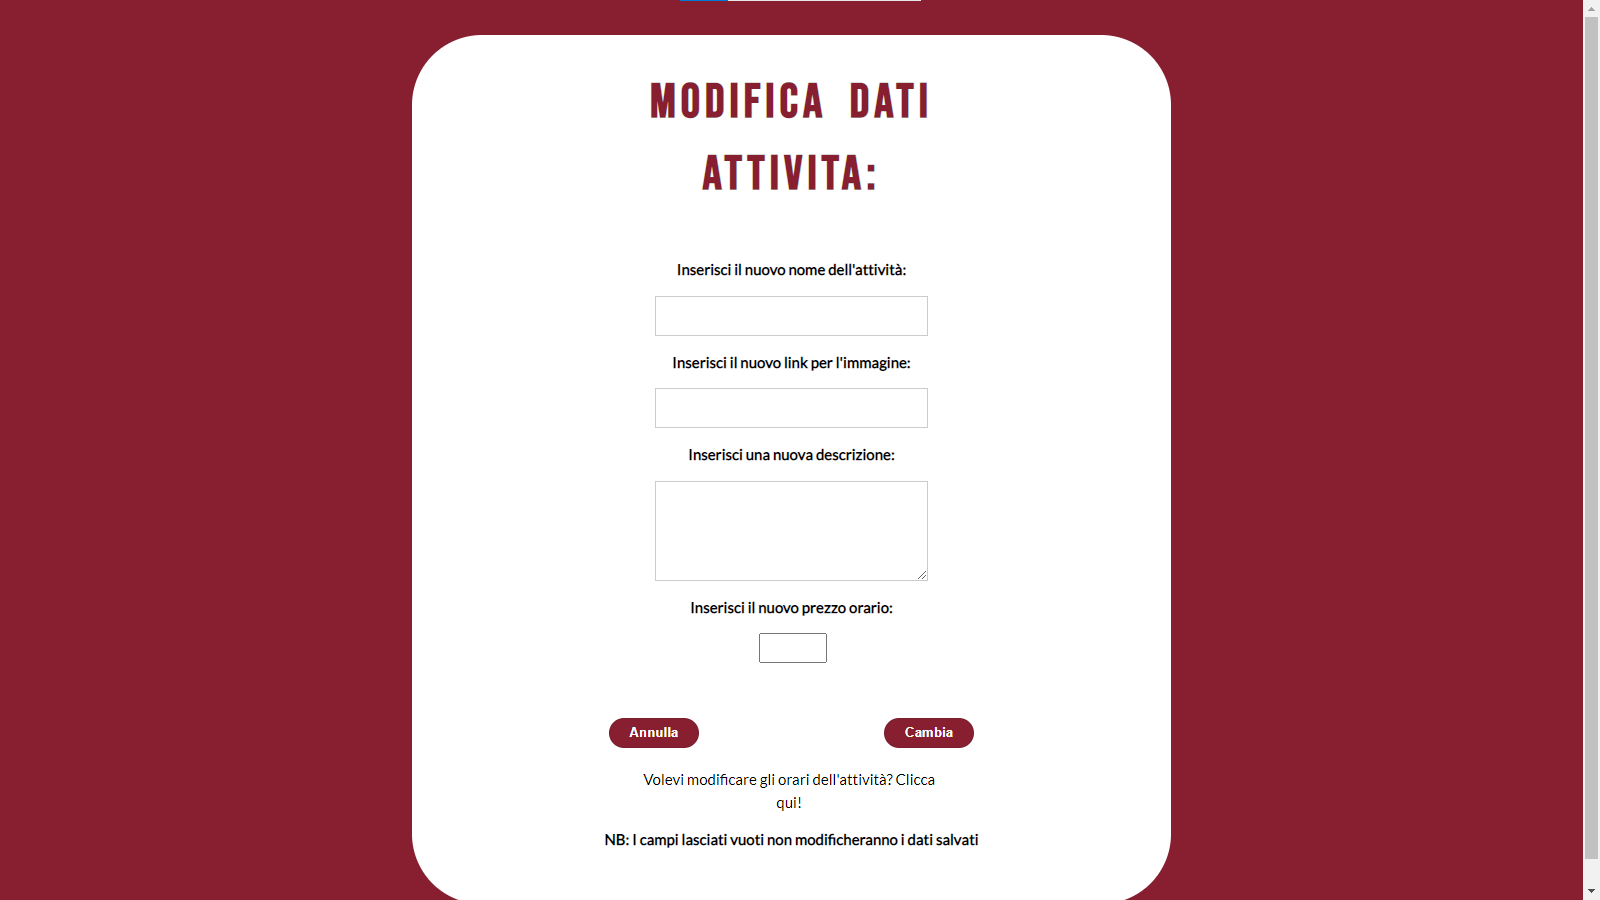
\includegraphics[scale=0.3]{ModificaAttivita.png}
\caption{Modifica dei dati di un'attività}
\label{ModificaAttivita}
\end{figure}\pagebreak

\subsection{Visualizzare le prenotazioni del servizio di ristorazione, modificarle ed annullarle}
\begin{figure}[!h]
\centering

\includegraphics[scale=0.3]{PrenotazioniClienti.png}
\caption{Pagina per scegliere le prenotazioni dei clienti da visualizzare}
\label{PrenotazioniClienti}
\end{figure}
Interagendo con il link \textbf{"VISUALIZZA PRENOTAZIONI CLIENTI"} si verrà portati nella pagina mostrata in figura \ref{PrenotazioniClienti}. Successivamente, cliccando sulla scritta \textbf{"PRENOTAZIONI RISTORANTE"} la concierge può visualizzare a schermo, in ordine cronologico (dalla prenotazione più prossima a quella meno), tutte le prenotazioni dei clienti suddivise in:
\begin{itemize}
\item \textbf{Stato:} attive o passate;
\item \textbf{Per tipo:} servizio in camera o servizio al tavolo.
\end{itemize} 
La pagina appena descritta è mostrata in figura \ref{PrenotazioniRistoranteStaff}\newpage
\begin{figure}[h]
\centering
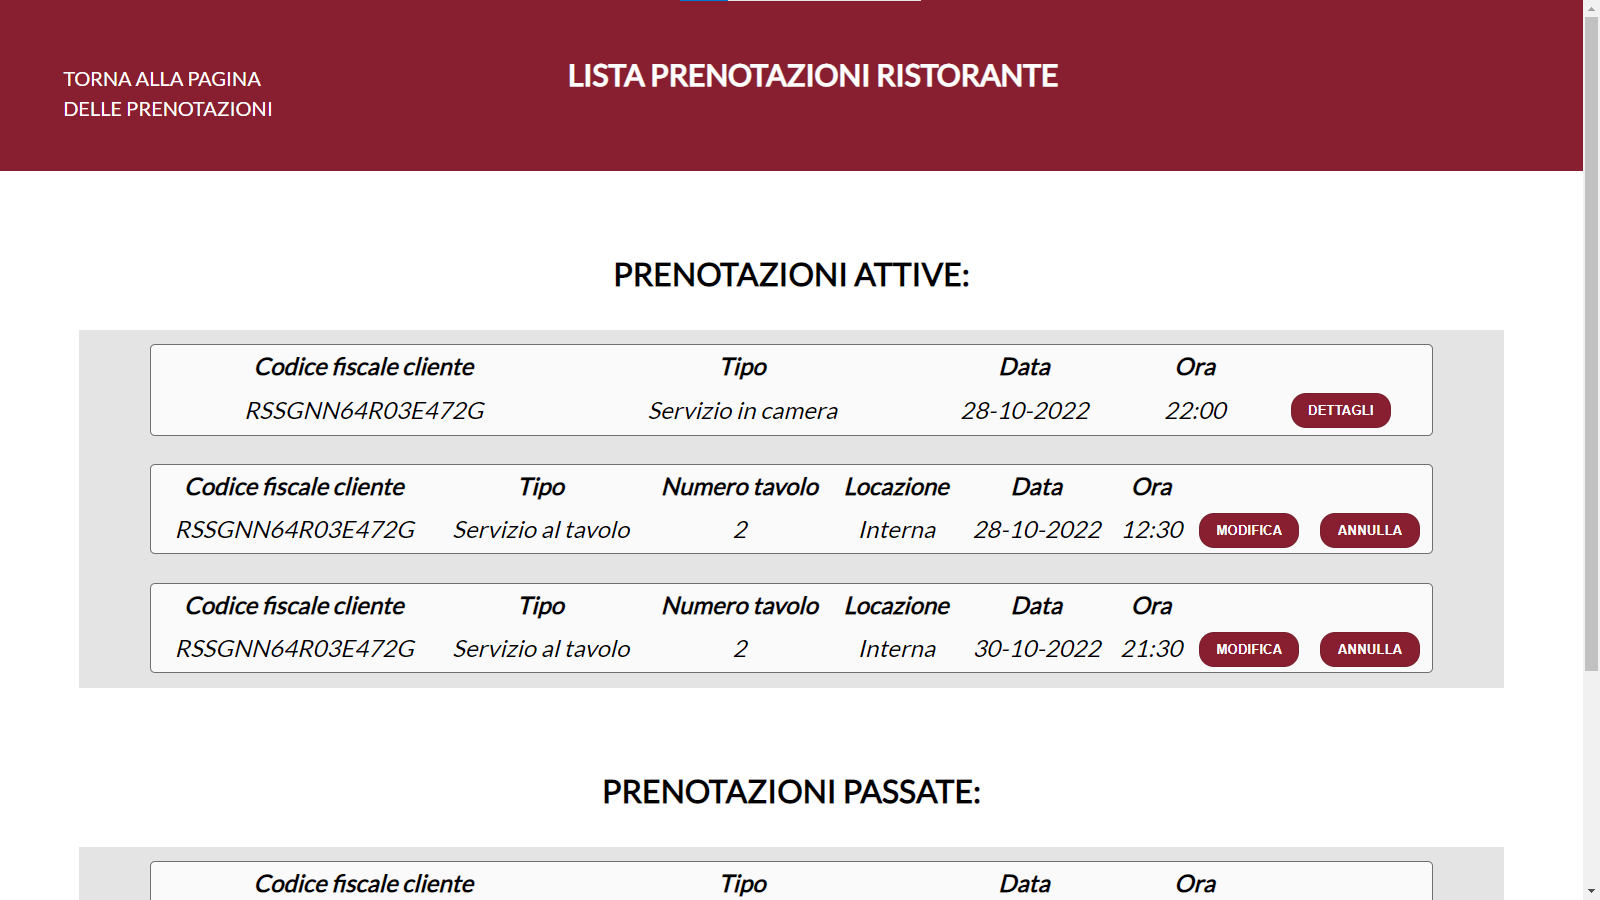
\includegraphics[scale=0.3]{PrenotazioniRistoranteStaff.png}
\caption{Lista delle prenotazioni del ristorante di tutti i clienti}
\label{PrenotazioniRistoranteStaff}
\end{figure}
Le prenotazioni con servizio in camera dispongono di un bottone denominato \textbf{"dettagli"} attraverso il quale la concierge può richiedere di visualizzare maggiori informazioni riguardo ad esse, e in caso siano prenotazioni attive, in seguito anche decidere di: \underline{aggiungere una portata}, \underline{eliminare una portata}, \underline{modificare la data e/o l'ora} o \underline{annullare} definitivamente la prenotazione. Per ognuna di queste opzioni la concierge dispone di bottoni specifici come mostrato nella figura \ref{DettagliPrenotazioneSCStaff}.
\begin{figure}[h]
\centering
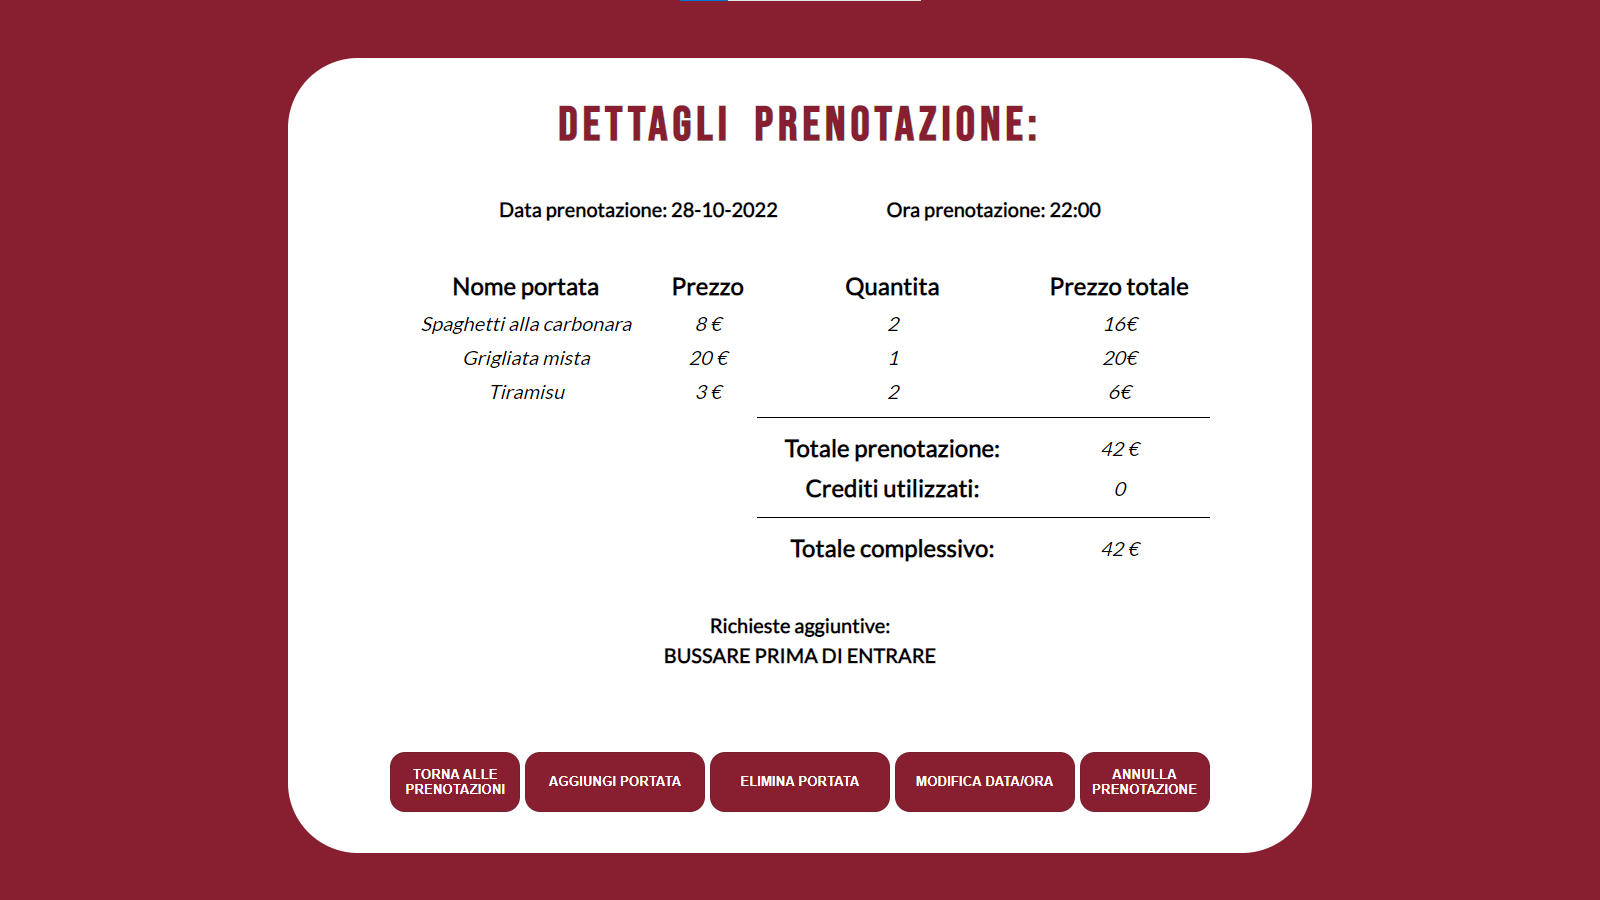
\includegraphics[scale=0.25]{DettagliPrenotazioneSCStaff.png}
\caption{Dettagli di una prenotazione attiva di un servizio in camera}
\label{DettagliPrenotazioneSCStaff}\pagebreak
\end{figure}
Nel caso in cui decidesse di aggiungere una portata, gli verrà chiesto di selezionarne una tra quelle presenti nel menù, con il numero delle portate associato. Esempio nella figura \ref{AggiungiPortataPrenotazioneSC}.\\\\
Nel caso in cui volesse eliminare una portata, gli verrà chiesto quale portata tra quelle presenti nella prenotazione eliminare, e in base al numero di porzioni ordinate dal cliente, il numero di porzioni da rimuovere. Esempio nella figura \ref{EliminaPortata}.\\\\
Per modificare la data e l'ora, come mostrato nell'esempio in figura \ref{ModificaDataOraPrenotazioneSC}, potrà selezionare una nuova data per la prenotazione (verranno rese selezionabili unicamente le date presenti nel soggiorno approvato del cliente). Potrà invece cambiare l'orario solamente dopo aver deciso la tipologia del pasto, ovvero pranzo o cena.\\\\
Infine, potrà annullare la prenotazione cliccando sul bottone appropriato e confermando la propria decisione sul pop-up che comparirà sul lato superiore dello schermo.\\\\
\begin{figure}[h]
\centering
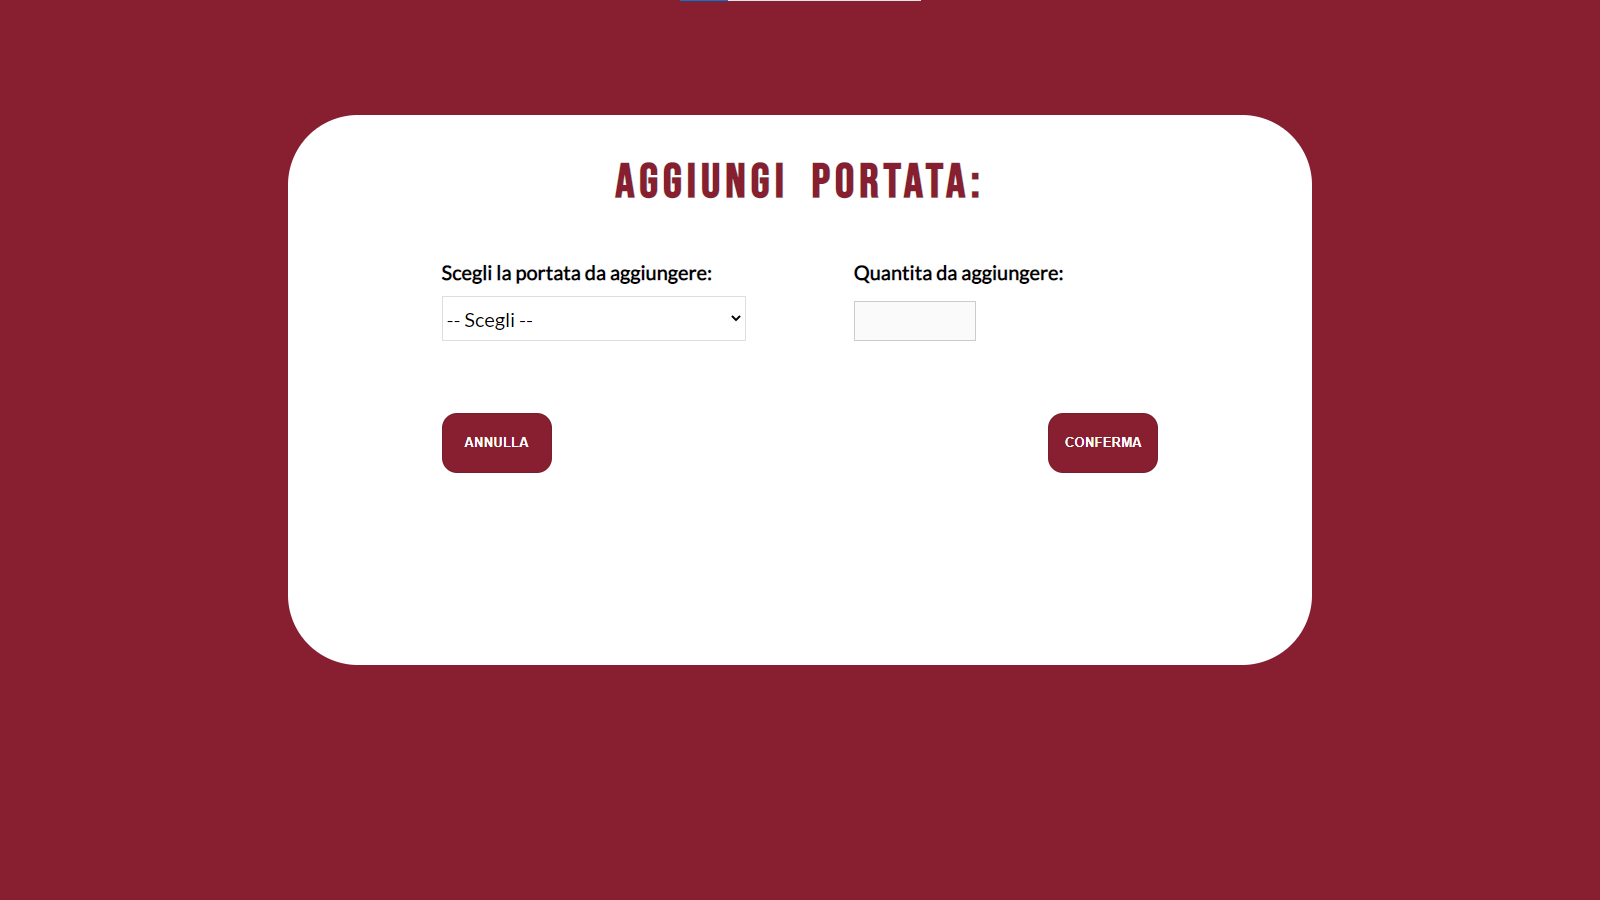
\includegraphics[scale=0.3]{AggiungiPortataPrenotazioneSC.png}
\caption{Aggiunta di una portata ad una prenotazione di un servizio in camera}
\label{AggiungiPortataPrenotazioneSC}
\end{figure}\newpage

\begin{figure}[h]
\centering
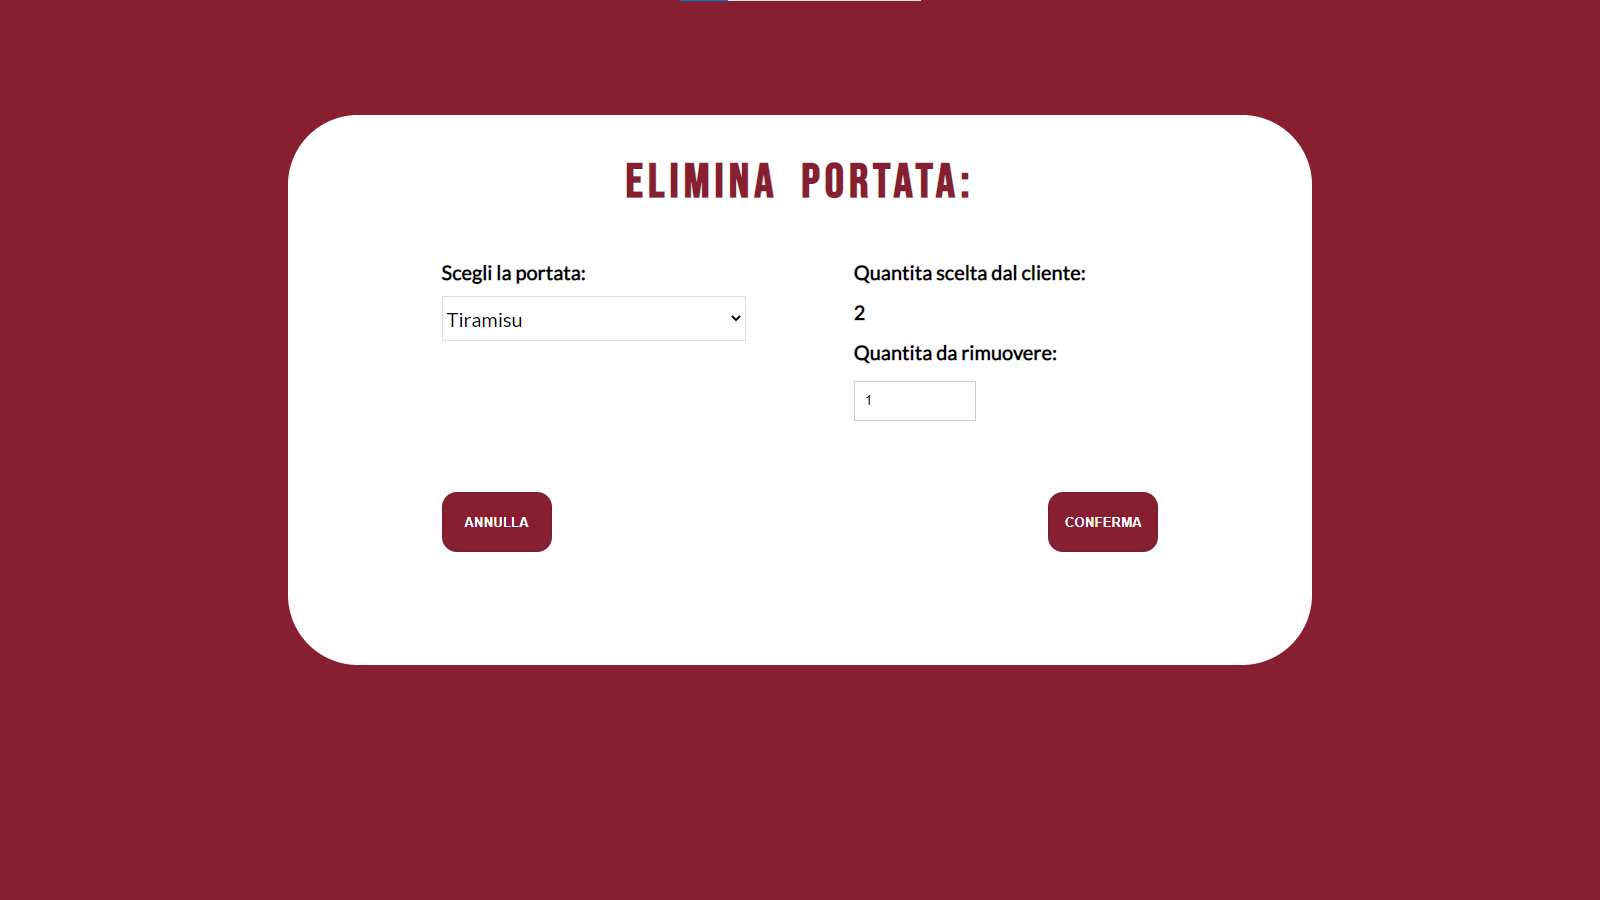
\includegraphics[scale=0.3]{EliminaPortata.png}
\caption{Rimozione di una certa quantità di una portata da una prenotazione di un servizio in camera}
\label{EliminaPortata}
\end{figure}

\begin{figure}[h]
\centering
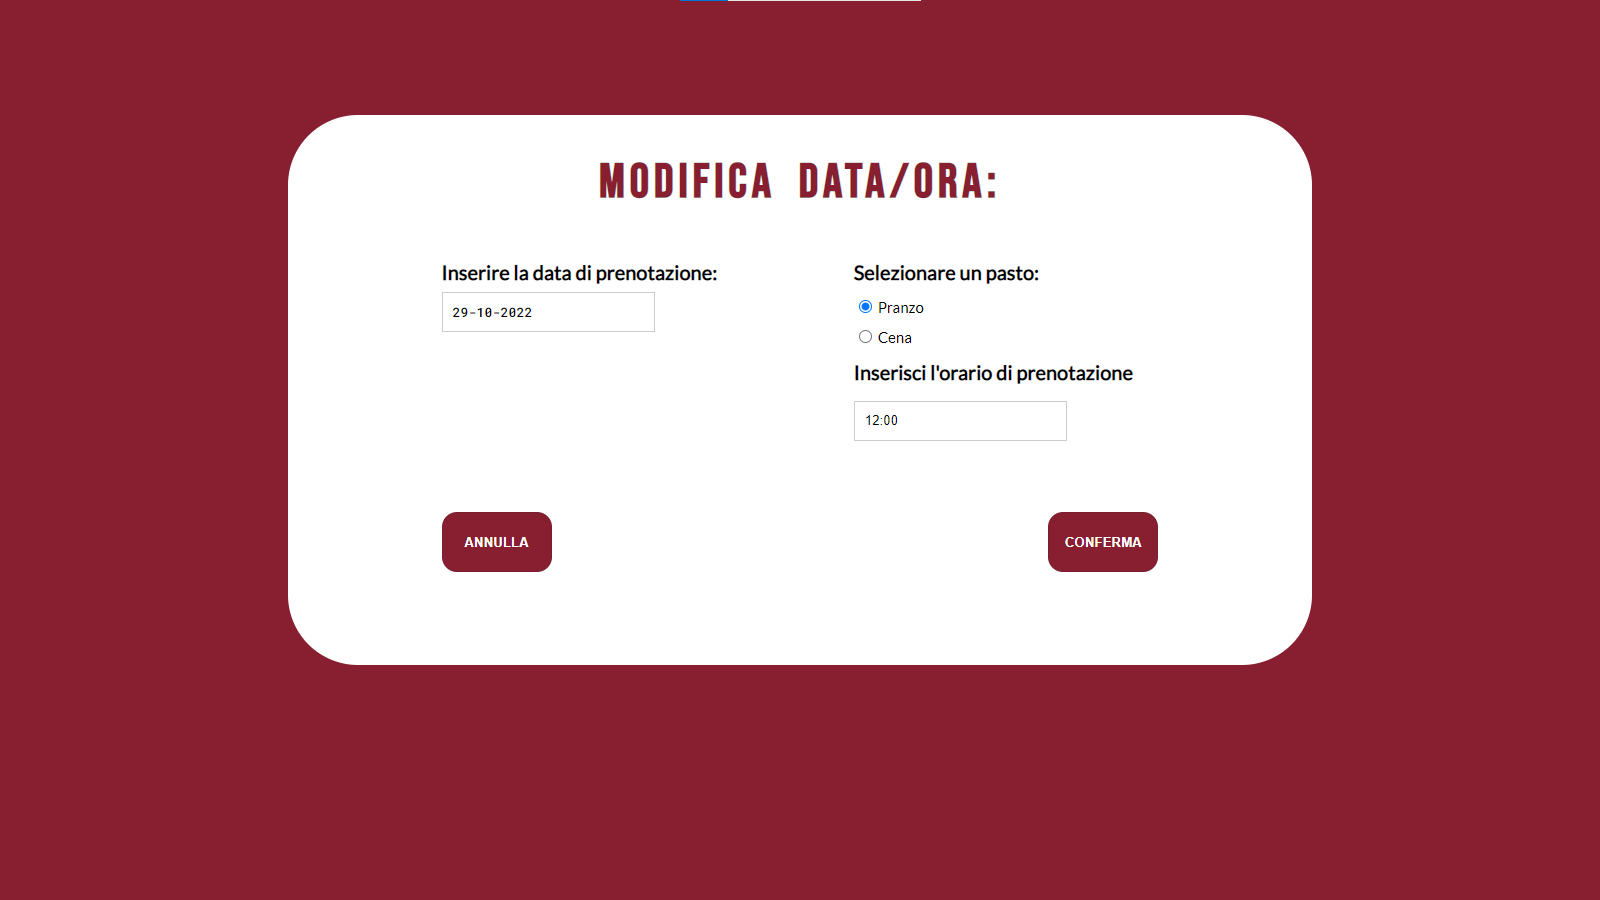
\includegraphics[scale=0.2]{ModificaDataOraPrenotazioneSC.png}
\caption{Modifica della data e/o ora di una prenotazione di un servizio in camera}
\label{ModificaDataOraPrenotazioneSC}
\end{figure}

Per le prenotazioni di servizio al tavolo invece, verranno mostrati direttamente sulla pagina della lista delle prenotazioni i due bottoni per modificare ed annullare la prenotazione, collocati sempre al di fianco di essa. Cliccando su \textbf{"modifica"} verrà chiesto alla concierge di modificare la \underline{data della prenotazione}, di scegliere una \underline{locazione} (interna o esterna), di selezionare la tipologia di pasto (pranzo o cena), e di selezionare un \underline{orario} specifico successivamente. L'utente potrà, una volta inserito correttamente tutti i dati, confermare o annullare le modifiche appena effettuate con i bottoni appropriati. Un esempio è riportato nella figura \ref{ModificaPrenotazioneTavolo}. \\\\
Cliccando invece su \textbf{"annulla"} e successivamente su \textbf{"ok"} nel pop-up che sarà comparso nella parte superiore della pagina per confermare la scelta intrapresa, la prenotazione verrà definitivamente cancellata.

\begin{figure}[h]
\centering
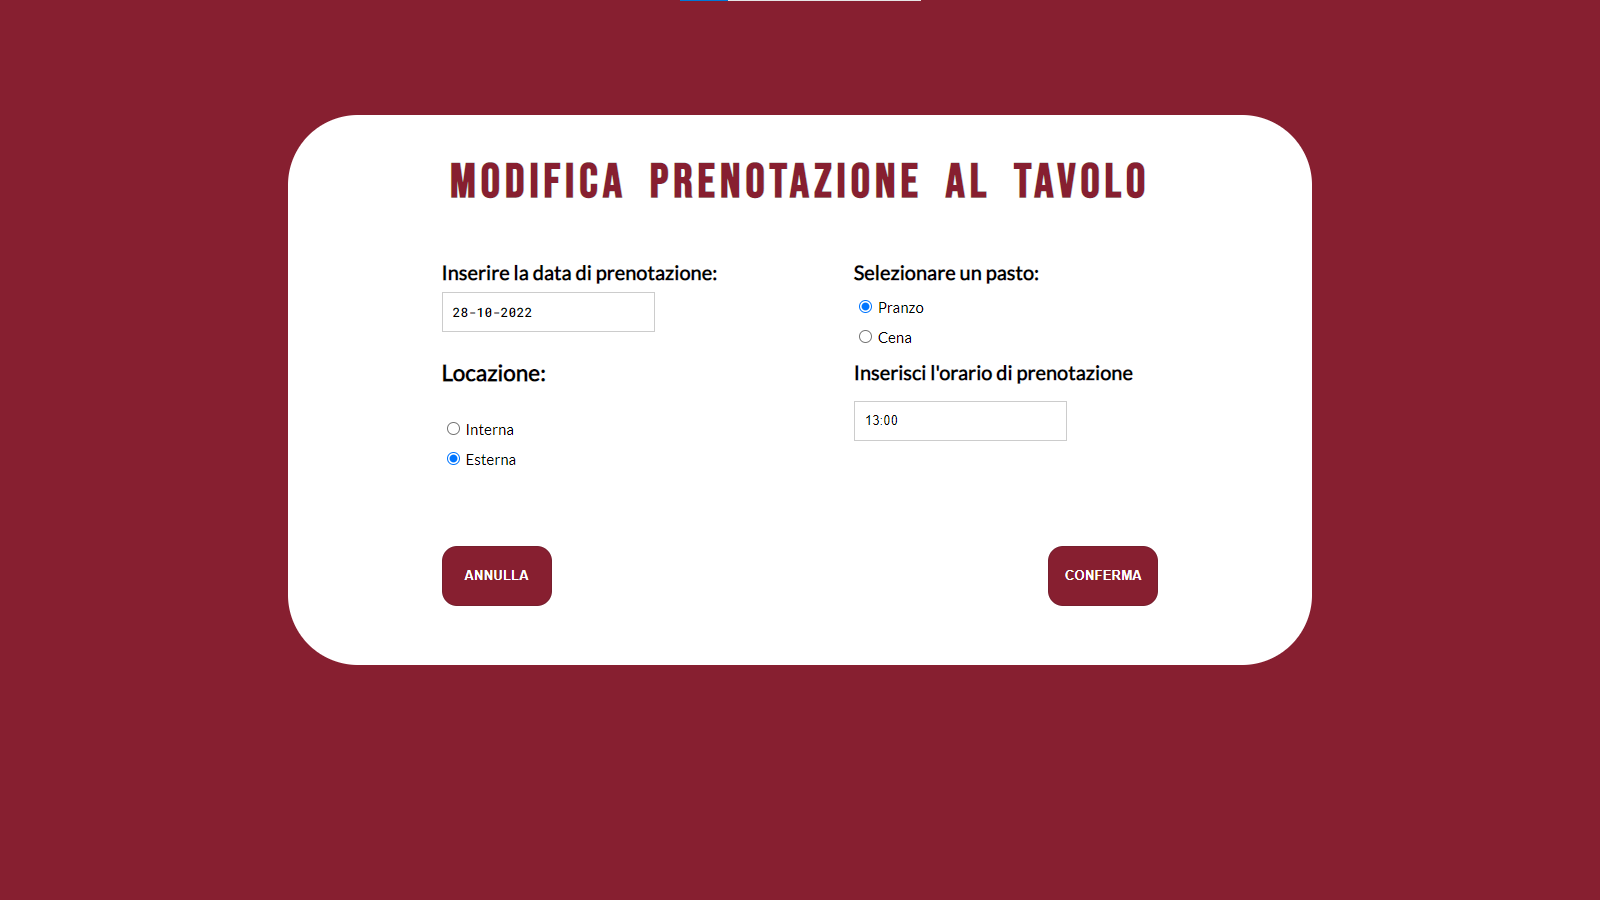
\includegraphics[scale=0.3]{ModificaPrenotazioneTavolo.png}
\caption{Modifica dei dati di una prenotazione del servizio al tavolo}
\label{ModificaPrenotazioneTavolo}
\end{figure}

\subsection{Visualizzare le prenotazioni delle attività, modificarle e annullarle}
Interagendo con il link \textbf{"PRENOTAZIONI ATTIVITÀ"} nella pagina mostrata in figura \ref{PrenotazioniClienti} la concierge può visualizzare a schermo, in ordine cronologico (dalla prenotazione più prossima a quella meno), tutte le prenotazioni delle attività dei clienti con le relative informazioni, suddivise per stato attivo o passato. Quest'ultime chiaramente verranno solamente visualizzate, mentre per le prime ci sarà la possibilità di modificarle o di annullarle. La pagina che mostra tutte le prenotazioni è mostrata in figura \ref{ListaPrenotazioniAttivitaStaff}   \newpage

\begin{figure}[h]
\centering
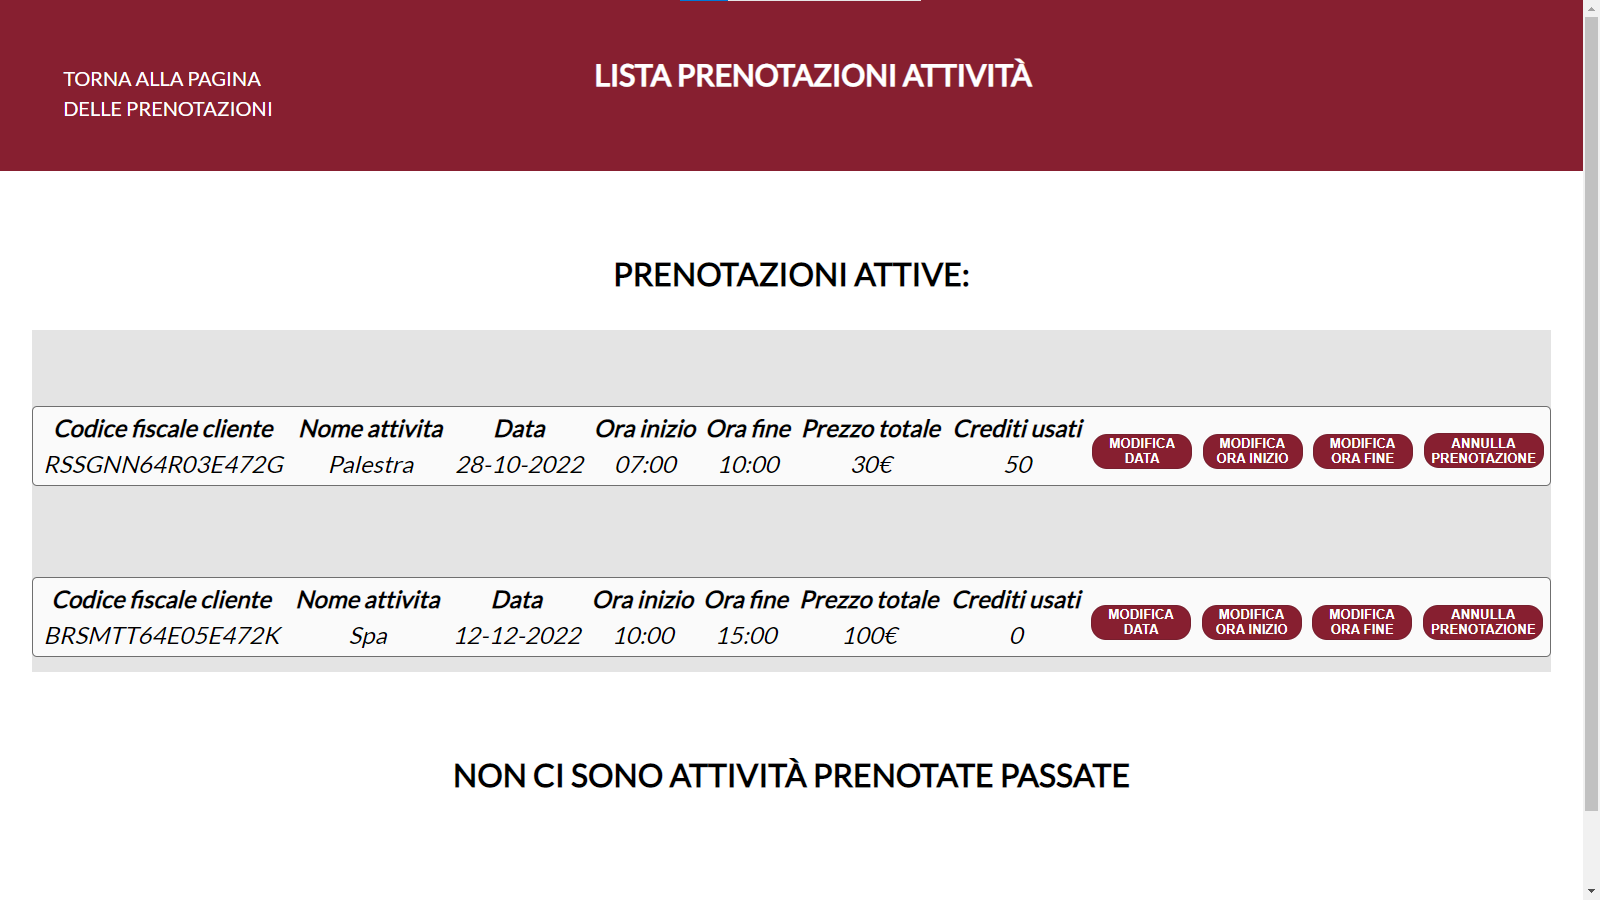
\includegraphics[scale=0.3]{ListaPrenotazioniAttivitaStaff.png}
\caption{Lista delle prenotazioni delle attività di tutti i clienti}
\label{ListaPrenotazioniAttivitaStaff}
\end{figure}

Per ogni prenotazione attiva, vengono mostrati quattro bottoni per poter modificare la data, l'ora di inizio e l'ora di fine prenotazione e per annullare la prenotazione.
Se la volontà della concierge è quella di modificare le prenotazioni attive, non dovrà fare nient'altro che cliccare sul apposito bottone relativo alla modifica che intende compiere .La modifica degli orari influenzerà anche il prezzo totale, il quale verrà ricalcolato in base ai nuovi dati inseriti.\\\\
Invece, se la volontà è quella di annullare una prenotazione, la concierge non dovrà far altro che cliccare sul bottone \textbf{"annulla prenotazione"} posizionato al di fianco di essa. In questo caso, come già spiegato nelle sottosezioni precedenti, dovrà successivamente confermare la decisione intrapresa cliccando su \textbf{"ok"} nel pop-up che sarà comparso nella parte superiore della pagina.


\subsection{Rispondere alle domande ed elevarle a FAQ}
La Concierge ha sicuramente un ruolo principale nel forum delle domande di cui fanno parte tutti i clienti registrati nella piattaforma. Accedendo attraverso il link \textbf{"DOMANDE"} collocato nella propria area utente, oltre a rispondere ad una domanda, come già spiegato nella sottosezione 2.2.11, essa potrà elevare a FAQ una qualsiasi domanda, ritenuta da lei meritevole di questo titolo. Per fare ciò, non dovrà far altro che cliccare sul bottone \textbf{"eleva a FAQ"}, collocato nella parte inferiore destra di ogni domanda come mostrato nella figura \ref{DomandeStaff}. Se il bottone non dovesse essere presente, vorrà dire che quella specifica domanda è già stata selezionata come FAQ. Elevando a FAQ una domanda, verrà inoltre consegnato un premio al cliente autore pari a cento crediti.  

\begin{figure}[h]
\centering
\includegraphics[scale=0.3]{DomandeStaff.png}
\caption{Pagina delle domande - Concierge}
\label{DomandeStaff}
\end{figure}

\subsection{Aggiungere, modificare o rimuovere una FAQ}

\begin{figure}[h]
\centering
\includegraphics[scale=0.25]{FaqStaff.png}
\caption{Pagina delle FAQ - Concierge}
\label{FaqStaff}
\end{figure}
Nella homepage del sito, interagendo con il link \textbf{"FAQ"}, la concierge potrà, oltre che visualizzare le FAQ presenti nella pagina, aggiungerle, modificarle o annullarle. La pagina, dal punto di vista del nostro utente, avrà un aspetto come quello mostrato nella figura \ref{FaqStaff}.\\\\
Nel caso esso voglia aggiungere una FAQ, non dovrà far altro che cliccare sulla scritta \textbf{"AGGIUNGI FAQ"} nella parte superiore destra della pagina e, successivamente, compilare con del testo, i campi di domanda e di risposta, come mostrato nell'esempio in figura \ref{AggiungiFaq}. Dovranno obbligatoriamente essere compilati entrambi i campi.\\\\
Se l'intento è quello di modificarla, allora bisognerà cliccare sul bottone \textbf{"modifica faq"}, collocato al di fianco di essa. L'unico campo modificabile sarà quello della risposta. Esempio mostrato nella figura \ref{ModificaFaq}.\\\\
Infine, per eliminarla, la concierge dovrà cliccare sul bottone \textbf{"rimuovi faq"}, anche esso collocato di fianco alla specifica FAQ, e dopo aver confermato la propria decisione, essa sarà rimossa dalla pagina. 

\begin{figure}[h]
\centering
\includegraphics[scale=0.3]{AggiungiFaq.png}
\caption{Aggiunta di una faq}
\label{AggiungiFaq}
\end{figure}\newpage

\begin{figure}[h]
\centering
\includegraphics[scale=0.3]{ModificaFaq.png}
\caption{Modifica di una faq}
\label{ModificaFaq}
\end{figure}

\section{Admin}
In questa sezione andiamo ad analizzare tutte le funzionalità usufruibili dal tipo di utenza \textbf{"Admin"}.\\\\
Assumiamo che l'utente visitatore si sia autenticato come Admin attraverso la pagina di login. Dopo aver fatto l'accesso, la schermata iniziale sarà quella dell'area dell'admin, come mostrato nella figura \ref{AreaAdmin}. 

\begin{figure}[h]
\centering
\includegraphics[scale=0.24]{AreaAdmin.png}
\caption{Area personale dell'admin}
\label{AreaAdmin}
\end{figure}\newpage
Come per l'area cliente e l'area concierge, l'area admin presenta la medesima struttura. Possiamo trovare nella sezione verticale di sinistra, quella di principale interesse, una grande somiglianza con quella della concierge; infatti, tutte le funzioni che caratterizzano questo tipo di utenza fanno parte anche di quella dell'admin. Quest'ultimo però presenta ulteriori funzionalità, così da renderlo il gestore principale della piattaforma. Andremo ora ad analizzare in dettaglio quest'ultime.

\subsection{Attivare, disattivare e aggiungere una categoria}
\begin{figure}[h]
\centering
\includegraphics[scale=0.3]{Categorie.png}
\caption{Pagina delle categorie}
\label{Categorie}
\end{figure}
Prima funzionalità che caratterizza un admin rispetto agli altri tipi di utenza è quella di avere la possibilità di attivare, disattivare e aggiungere una categoria. 
Interagendo con il link \textbf{"CATEGORIE"} presente nell'area admin, esso verrà indirizzato in un'altra pagina, come quella in figura \ref{Categorie}. Qui potrà visualizzare tutte le categorie presenti nella piattaforma divise per stato (attive o disabilitate).\\\\
Per quelle con stato attivo '’utente in questione potrà, cliccando sul bottone \textbf{"Disattiva"} collocato al di fianco della categoria scelta, disabilitarla.\\\\ 
D'altra parte, egli potrà, per quelle con stato disabilitato, cliccare sul bottone \textbf{"Attiva"} collocato anch'esso al di fianco della categoria scelta per attivarla. \\\\
Infine, cliccando sul bottone \textbf{"Aggiungi"} sul fondo della pagina, gli sarà permesso di aggiungere una nuova categoria e, per farlo, dovrà scrivere il nome nell' apposito campo come mostrato nell'esempio in figura \ref{AggiungiCategoria}. Dovrà inoltre selezionare le azioni che saranno correlate ad essa.

\begin{figure}[h]
\centering
\includegraphics[scale=0.3]{AggiungiCategoria.png}
\caption{Aggiunta di una nuova categoria}
\label{AggiungiCategoria}
\end{figure}

\subsection{Approvare o rifiutare un pagamento}
\begin{figure}[h]
\centering
\includegraphics[scale=0.25]{Pagamenti.png}
\caption{Lista dei pagamenti dei clienti}
\label{Pagamenti}
\end{figure}
Appena il cliente effettua una prenotazione di un soggiorno, tale prenotazione deve essere approvata dall'admin, il quale appunto ha l'intero diritto di scegliere se approvare o rifiutare il pagamento di quest'ultimo, o in altre parole, il suo soggiorno. \\\\
Per fare ciò, nella propria area utente, l'admin dovrà interagire con il link \textbf{"PAGAMENTI CLIENTI"}. È qui che verrà indirizzato in una nuova pagina, figura \ref{Pagamenti}, nella quale potrà visionare la lista dei soggiorni (ad eccezioni di quelli terminati), divisi per stati (approvati, pagamenti sospesi e rifiutati), di tutti i clienti registrati nella piattaforma con tutte le relative informazioni associate. È logico pensare che siano i soggiorni con stato \textbf{"Pagamento sospeso"} gli unici con la caratteristica di poter essere approvati o rifiutati. 
Per approvare un pagamento, l'admin non dovrà far altro che cliccare sul bottone \textbf{"approva"} situato al di fianco del soggiorno scelto. Nel caso contrario basterà invece cliccare sul bottone \textbf{"rifiuta"}. 

\subsection{Visualizzare i clienti e modificarne i dati}
\begin{figure}[h]
\centering
\includegraphics[scale=0.3]{ListaClienti.png}
\caption{Lista dei clienti registrati all'interno del sito}
\label{ListaClienti}
\end{figure}
Ulteriore funzione dell'admin è quella di poter visualizzare tutti i clienti registrati nella piattaforma e di modificarne dati e credenziali.\\\\
Cliccando sul link \textbf{"VISUALIZZA CLIENTI"} nella propria area utente, esso potrà visionare tutti i clienti registrati sulla piattaforma. Come possiamo vedere dalla figura \ref{ListaClienti}, essi verranno divisi in clienti presenti all'interno della struttura (ovvero che possiedono un giorno del loro soggiorno attivo che coincide con il giorno in cui l'admin sta visualizzando la pagina) e non presenti in struttura.\\\\
Per ognuno dei clienti ci sarà la possibilità di poter modificare i relativi dati, cliccando sul simbolo della matita collocato al di fianco del cliente scelto. In questo modo l'admin potrà accedere ad una pagina apposita, analoga alla pagina dei dati personali di un cliente mostrata in figura \ref{DatiPersonali}, con la differenza che non verranno mostrate le informazioni riguardante i soggiorni.\\\\ 
In tale pagina, si potrà cambiare un dato alla volta cliccando sul medesimo simbolo situato al di fianco del dato scelto da modificare, in modo completamente analogo alla modifica dei dati personali descritta nella sottosezione 2.2.15


\subsection{Modificare gli orari di update del menù}
\begin{figure}[h]
\centering
\includegraphics[scale=0.3]{ListaOrariAdmin.png}
\caption{Lista degli orari - Admin}
\label{ListaOrariAdmin}
\end{figure}
Oltre alla funzione di modificare gli orari di apertura e di chiusura del ristorante e delle attività, come già analizzato in modo dettagliato nella sottosezione 2.3.2 della concierge, nella pagina della modifica degli orari, raggiungibile nel medesimo modo, verrà mostrato all'admin la possibilità di modificare gli orari di update del menù del ristorante, come si può notare dalla figura \ref{ListaOrariAdmin}.\\\\ 
Cliccando sul bottone \textbf{"modifica"} collocato al di fianco agli orari di update, l'utente sarà in grado di scegliere i nuovi orari di inizio e di fine update. Esempio nella figura \ref{ModificaOrariUpdate}. Devono essere obbligatoriamente inseriti entrambi gli orari, i quali non dovranno interferire con i range orari del pranzo e della cena. Verranno accettate unicamente modifiche logicamente sensate. 
\begin{figure}[h]
\centering
\includegraphics[scale=0.3]{ModificaOrariUpdate.png}
\caption{Modifica degli orari di update del menù}
\label{ModificaOrariUpdate}
\end{figure}









\chapter{Programmazione}
In questo capitolo verranno analizzati i vari script che costituiscono il sito web. In particolare, per comodità essi possono essere divisi in due macro-categorie:
\begin{enumerate}
\item \textbf{Script delle pagine:} sono script php contenuti direttamente nelle pagine stesse visualizzate dagli utenti, i cui compiti principali sono: manipolare i dati della pagina, controllare i dati inseriti dall'utente (ed eventualmente della loro correttezza), impostare variabili di sessione, controllare la legalità degli accessi, richiamare gli script delle funzioni ed effettuare il reindirizzamento dell'utente ad altre pagine.
\item \textbf{Script delle funzioni:} essi sono script incapsulati all'interno di funzioni PHP e memorizzati all'interno di appositi file dedicati, non accessibili da nessuna tipologia di utente. Essi sono divisi a loro volta in cinque categorie: 
\begin{enumerate}
\item \textbf{Funzioni Get:} funzioni il cui compito sarà quello di estrarre dati dai file XML ed, in alcuni casi, effettuare dei controlli sui dati estratti.
\item \textbf{Funzioni Modifica:} funzioni il cui compito sarà quello di modificare dei dati già esistenti in un file XML
\item \textbf{Funzioni Insert:} funzioni che andranno ad inserire nuovi dati all'interno di un file XML
\item \textbf{Funzioni delete:} funzioni che andranno a rimuovere dei dati da un file XML
\item \textbf{Funzioni PHP:} funzioni generiche che sono necessarie per il funzionamento del sistema ma non catalogabili in una categoria particolare.
\end{enumerate}
\end{enumerate}

\section{Script delle pagine}
In questa sezione verranno analizzati i vari script contenuti all'interno delle pagine del sito e verrà descritto il loro funzionamento. Per motivi pratici, non verranno esaminate le pagine contenenti esclusivamente script di controllo della legalità dell'accesso


\subsubsection{registrazioneUtente.php}
Lo script contenuto all'interno di questa pagina avrà come scopo principale quello di verificare che l'utente abbia inserito tutti i dati richiesti al momento della registrazione ed, in particolare, della loro correttezza (il codice fiscale deve rispettare un determinato pattern, così come il numero di carta di credito, la mail, ecc..).  Se tutti i dati inseriti sono corretti allora egli passerà a controllare, mediante la chiamata delle funzioni \textit{getCodFisc} e \textit{getUsername}, la presenza di eventuali duplicati del codice fiscale o dell'username inseriti. Se anche quest'ultimi due controlli vanno a buon fine allora si andrà a registrare effettivamente l'utente nel file XML mediante la chiamata della funzione \textit{inserisciNuovoCliente}.

\subsubsection{login.php}
Poiché questa pagina potrà essere aperta in due situazioni differenti (normalmente dalla pagina home oppure automaticamente durante la prenotazione di un soggiorno se l'utente non ha già effettuato il login) il primo scopo di questo script sarà quello di distinguere questi due casi. Ciò viene fatto andando a controllare se la variabile di sessione \textit{prenotazioneCamera} è settata:
\begin{enumerate}
\item In caso negativo, allora verrà visualizzata la normale pagina di login. Dopo aver controllato che l'utente abbia inserito tutti i dati, lo script richiamerà la funzione \textit{eseguiLoginCliente} oppure la funzione \textit{eseguiLoginStaff} dipendentemente da quale tipologia di utente è stata selezionata nella pagina. Se il login del cliente va a buon fine, allora verranno impostate tre variabili di sessione che verranno poi utilizzate dalle altre pagine:
\begin{enumerate}
\item \textit{loginType} (per distinguere il tipo di login che è stato effettuato).
\item \textit{codFiscUtenteLoggato}: verrà passata come parametro ad alcune funzioni presenti nelle varie pagine.
\item \textit{soggiornoAttivo:} memorizza al suo interno la presenza o meno di un soggiorno attivo associato al cliente, cioè con pagamento sospeso oppure con stato \textit{approvato} (un valore \textit{"null"} equivale a dire che il cliente non ha un soggiorno attivo).
\end{enumerate}  
Se invece dovesse andare a buon fine il login del concierge o dell'admin allora sarà sufficiente settare solamente la variabile di sessione \textit{loginType} (il cui valore dipende da quale tipologia di login è stata effettuata).
\item Nel caso in cui la variabile \textit{prenotazioneCamera} dovesse essere settata, allora significa che l'utente stava effettuando la prenotazione di una camera. Dopo aver estratto i dati della prenotazione per poterli salvare in dei campi input \textit{hidden} (in modo da non perderli), verrà visualizzata la normale pagina del login con delle piccole differenze: nella sezione verticale di sinistra verrà visualizzata una sola scritta per annullare la prenotazione in corso e nella sezione di destra non verrà data la possibilità di scegliere il tipo di utente (non si possono associare camere ad utenti registrati come concierge o admin). Il login dopodiché viene svolto normalmente ma con un controllo aggiuntivo: se le credenziali inserite dall'utente sono corrette allora si andrà a controllare, mediante la funzione \textit{getSoggiornoAttivo}, se l'utente che sta effettuando il login ha già un soggiorno attivo. In tal caso, non verrà concesso all'utente di continuare la prenotazione.
\end{enumerate} 

\subsubsection{visualizzaDisponibilita.php}
Questo script andrà prima di tutto a controllare che l'utente sia arrivato in questa pagina in modo legale (cioè inserendo prima delle date in \textit{prenotaOra.php}). Dopodiché, dopo aver estratto dalla variabile di sessione le due date scelte dall'utente, le andrà a passare come parametro alla funzione \textit{getCamereDisponibili}: sulla base del risultato di tale funzione verrà costruita una pagina contenenti tutte le camere che possono essere prenotate nel range temporale inserito dall'utente. Quando l'utente andrà a scegliere una camera, lo script richiamerà la funzione \textit{individuaBottoneCamereDisponibili} per poter individuare quale bottone è stato premuto ed ottenere l'id della camera ad esso associato. Infine, verrà controllato se la variabile di sessione \textit{codFiscUtenteLoggato} è settata: in caso affermativo, allora significa che l'utente ha già effettuato il login e dunque può essere portato nella pagina \textit{confermaPrenotazione.php} per completare la prenotazione. In caso negativo, l'utente verrà portato nella pagina di login.

\subsubsection{confermaPrenotazione.php}
Poiché in questa pagina verranno confermate le prenotazioni di un soggiorno oppure di un'attività, lo script andrà innanzitutto a distinguere quale tipologia di prenotazione l'utente stava effettuando mediante il controllo delle variabili di sessione \textit{prenotazioneCamera} e \textit{prenotazioneAttivita}. Dopo aver estratto i dati necessari che dovranno essere visualizzati all'utente, lo script andrà a costruire una pagina il cui contenuto sarà dipendente dal tipo di variabile di sessione che è stata trovata settata. Se l'utente conferma la prenotazione, allora essa verrà registrata mediante la chiamata della funzione \textit{inserisciPrenotazioneCamera} oppure di \textit{inserisciPrenotazioneAttivita}. Il controllo per capire quale funzione richiamare viene fatto in base a quale input type hidden è stato creato dalla pagina (ad esempio, nel caso della prenotazione di un camera verrà creato un input type hidden  il cui attributo \textit{name} sarà : \textit{idCamera}).

\subsubsection{datiPersonali.php}
Questa pagina potrà essere utilizzata in due circostanze diverse: 
\begin{enumerate}
\item Da un cliente che ha effettuato l'autenticazione e vi accede dalla propria area personale. In tal caso, verrà trovata settata la variabile di sessione \textit{codFiscUtenteLoggato} e dunque verranno estratti i dati personali del cliente mediante la funzione \textit{getDatiCliente} e tutti i soggiorni passati/rifiutati associati a quest'ultimo mediante la funzione \textit{getSoggiorniPassati}
\item Da un admin dopo che ha selezionato un particolare cliente di cui vuole visualizzare (ed eventualmente modificare) i dati personali. In tal caso verranno solamente estratti i dati personali del cliente.
\end{enumerate}
Dopodiché la pagina verrà costruita sulla base dei dati che sono stati estratti


\subsubsection{modificaDatiUtente.php}
Lo script di questa pagina è abbastanza articolato poiché qui si potrà modificare un qualsiasi dato personale di un cliente dell'hotel e saranno presenti tutti i controlli per i vari sottocasi a seconda del dato che si vuole modificare. Tuttavia, si potrà modificare un solo dato alla volta e dunque la pagina dovrà individuare il dato selezionato dall'utente per capire che cosa mostrare a schermo. Innanzitutto lo script richiamerà la funzione \textit{individuaDatoDaModificare} e salvare il suo risultato nella variabile PHP \textit{datoDaModificare}. Nel caso in cui tale variabile dovesse risultare pari a \textit{"null"} allora significa che non è stato trovato nessun dato da modificare selezionato dall'utente e dunque la pagina è stata aperta in modo illegale. Il corpo della pagina verrà poi costruito poi mediante \textit{switch} basato sul contenuto della variabile \textit{datoDaModificare}. Quando poi l'utente decide di confermare la modifica, lo script andrà ad eseguire una serie di controlli if basati sul tipo di dato che stava modificando.
\begin{enumerate}
\item Per il \textit{nome}, il \textit{cognome}, \textit{l'indirizzo}, la \textit{data di nascita} e l'\textit{username} sarà sufficiente controllare che il contenuto del campo testuale sia non vuoto.
\item Per il \textit{codice fiscale}, il \textit{telefono}, l'\textit{email} ed il \textit{numero della carta} sarà necessario controllare che il nuovo dato inserito rispetti un determinato pattern (dipendente dal tipo di dato).
\item Per la \textit{password} sarà necessario controllare innanzitutto che il contenuto dei due campi testuali (quello della vecchia password e quello della nuova) sia non vuoto. Dopodiché, nel caso in cui la vecchia password dovesse essere errata, lo script mostrerà un apposito messaggio d'errore.
\end{enumerate}
Oltre a questo, occorre mostrare dei messaggi d'errore nel caso in cui il nuovo codice fiscale inserito oppure il nuovo username siano duplicati (cioè già utilizzati da un altro utente). Il controllo dei duplicati e della correttezza della vecchia password sono entrambi implementati nella funzione \textit{modificaDatiUtente}. Lo script di questa pagina dovrà semplicemente controllare il valore della variabile \textit{result} che indicherà il successo o meno della modifica.






\subsubsection{prenotaTavolo.php}
Il primo passo dello script di questa pagina sarà la definizione della data minima e di quella massima che potranno essere inserite dall'utente per la prenotazione. In particolare:
\begin{enumerate}
\item La data minima viene decisa in base ad un confronto con la data odierna: se quest'ultima è maggiore della data di inizio soggiorno allora la data odierna sarà la minima data che potrà essere scelta. Altrimenti, la data di inizio soggiorno sarà quella minima.
\item La data massima che potrà essere scelta corrisponderà alla data di fine soggiorno.
\item Entrambe le date verranno invertite (cioè verranno scritte nell'ordine \textit{giorno - mese - anno}) in modo tale da renderle idonee per essere impostate come date minime e massime. Tale vincolo viene realizzato andando a passare le variabili php contenenti le date invertite a delle variabili \textit{javascript}. Con quest'ultimo si andrà poi ad impostare un \textit{datePicker} con le date che sono state passate.
\end{enumerate}
Sempre in questa pagina sarà poi presente un campo in cui l'utente potrà scegliere l'orario di prenotazione. Gli orari ammessi per effettuare una prenotazione vengono mostrati in base alla scelta dell'utente del pasto (\textit{pranzo} o \textit{cena}) ed ovviamente sulla base degli orari di apertura e di chiusura del ristorante. Se l'utente ha inserito tutti i dati lo script andrà a richiamare la funzione \textit{cercaTavoloDisponibile} per verificare se è presente o meno un tavolo in grado di soddisfare le richieste del cliente.

\subsubsection{prenotaSC.php}
Lo script di questa pagina andrà a costruire il campo della data e dell'orario per la prenotazione del servizio in camera in modo analogo a quanto detto in \textit{prenotaTavolo.php}. L'unica differenza sarà la presenza di un controllo aggiuntivo riguardante gli orari di modifica del menu: infatti, mediante la funzione \textit{confermaOraUpdateMenu} si andrà a verificare se l'ora corrente si trova all'interno del range orario di modifica del menù. In tal caso non verranno mostrati i campi per inserire la data e l'orario e l'utente non avrà la possibilità di proseguire la prenotazione. Se l'utente invece inserisce correttamente la data e l'orario di prenotazione, lo script andrà a settare la variabile di sessione \textit{dettagliSC} che servirà per mantenere i dati appena inseriti e permettere l'accesso in \textit{listaPortate.php}

\subsubsection{listaPortate.php}
La pagina, dopo aver controllato che la variabile di sessione \textit{dettagliSC}, andrà a costruire una pagina per permettere all'utente di selezionare le portate da ordinare. Per farlo andrà a richiamare la funzione \textit{getPortate} ed estrarre dal risultato di tale funzione quattro array: un array contenente gli \textit{antipasti}, uno i \textit{primi piatti}, uno i \textit{secondi piatti} e infine l'ultimo contenente i \textit{dolci}. Sulla base del contenuto di questi quattro array la pagina verrà costruita di conseguenza. In particolare: una portata verrà considerata selezionata ed aggiunta all'ordine esclusivamente se l'utente spunta la relativa casella associata. Quando un utente spunta una casella, grazie ad un codice \textit{javascript}, si andrà ad attivare la relativa casella della quantità, che di default sarà impostata ad 1 (l'utente poi avrà la possibilità solo di aumentare tale numero). Al momento della conferma, lo script andrà a richiamare la funzione \textit{individuaPortateSelezionate} che restituirà un array contenente tutte le portate scelte dall'utente e con la relativa quantità. Infine si andrà ad impostare la variabile di sessione \textit{richiestaSC} che, oltre a contenere tutti i dati inseriti dall'utente, permetterà l'accesso alla pagina \textit{dettagliPrenotazioneSC.php}

\subsubsection{dettagliPrenotazioneSC.php}
Questa pagina potrà essere aperta legalmente in tre situazioni differenti:
\begin{enumerate}
\item Quando l'utente deve completare la prenotazione di un servizio in camera. In tal caso verrà trovata settata la variabile di sessione \textit{richiestaSC}. Lo script andrà a richiamare la funzione \textit{getDatiCliente} in modo tale da ottenere gli eventuali crediti che il cliente dispone, mostrarli a schermo e permettere di utilizzarli per integrare il pagamento della prenotazione. Per permettere ulteriori controlli in altre porzioni del codice verrà inoltre settata la variabile \textit{confermaPrenotazione}. Il valore di quest'ultima non è importante, sarà sufficiente controllare che essa sia settata per distinguere le tre tipologie di accesso differenti (ad esempio grazie ad essa verranno creati solamente il bottone di annulla e conferma ed alcuni input type \textit{hidden} per poter completare la prenotazione).
\item Quando l'utente vuole ottenere i dettagli di una sua prenotazione attiva o passata. In questo caso verrà trovata settata la variabile di sessione \textit{dettagliSC}. Poiché tale variabile contiene solamente l'id della prenotazione selezionata dal cliente, l'id verrà passato alla funzione \textit{getPrenotazioneServizioCamera} in modo tale da ottenere tutti i dati da mostrare a schermo. Verrà poi settata la variabile \textit{dettagliPrenotazione} (logica analoga a quella di \textit{confermaPrenotazione} del caso precedente). Per distinguere infine una prenotazione attiva da una passata si andrà semplicemente ad effettuare un confronto con la data odierna: se quest'ultima è precedente alla data di prenotazione allora verrà mostrato all'utente il bottone per poter eventualmente annullare la prenotazione.
\item Quando la concierge o l'admin vogliono visualizzare i dettagli di una prenotazione di un servizio in camera ed eventualmente modificarla. Verrà di nuovo trovata settata la variabile di sessione \textit{dettagliSC} ma con una differenza: ora la variabile di sessione \textit{loginType} non sarà più pari a \textit{"Cliente"}. Pertanto, mediante un controllo della variabile \textit{loginType} si andrà a settare la variabile \textit{accessoStaff} che permetterà di mostrare i tre bottoni aggiuntivi per la modifica della prenotazione.
\end{enumerate}

\subsubsection{visualizzaPrenotazioniRistorante.php}
Lo script di questa pagina andrà a richiamare inizialmente la funzione \textit{getPrenotazioniRistorante} per ottenere tutte le prenotazioni da mostrare a schermo. La particolarità è che esso andrà anche a creare un input type \textit{hidden} con nome: \textit{bottonePremuto}. Infatti, ad inizio dello script il primo controllo che viene fatto è riguardante tale variabile POST:
\begin{enumerate}
\item Appena l'utente apre la pagina il controllo non andrà mai a buon fine, poiché non è ancora stata settata tale variabile.
\item Quando l'utente preme un qualsiasi bottone, la pagina verrà ricaricata e dunque tale variabile POST verrà trovata settata e si andrà ad individuare il bottone scelto dall'utente.
\end{enumerate}
In questo modo si evita un inutile ricerca di un eventuale bottone premuto ogni volta che si apre la pagina e, tale ricerca, verrà effettuata solo quando è stato effettivamente premuto un bottone.\\\\
Dopo la ricerca con la funzione \textit{individuaBottonePrenotazioniRistorante}, con la funzione \textit{strpos} si andrà ad analizzare l'id che è stato restituito in modo tale da poter capire se esso rappresenta l'id di una prenotazione di un servizio in camera oppure di un servizio al tavolo.
\begin{enumerate}
\item Nel caso del servizio al tavolo allora si controllerà se è stato settato un COOKIE con nome \textit{"Cancella"}. Esso verrà settato solamente se l'utente conferma la cancellazione della prenotazione nella finestra pop up che verrà mostrata dopo aver premuto il bottone. In caso affermativo si procede dunque a rimuovere il COOKIE (per evitare problemi per futuri controlli) ed a rimuovere la prenotazione mediante la funzione \textit{rimuoviPrenotazioneTavolo}.
\item Nel caso del servizio in camera invece si andrà semplicemente a settare la variabile di sessione \textit{dettagliSC} e si reindirizzerà l'utente in \textit{dettagliPrenotazioneSC}.
\end{enumerate}

\subsubsection{visualizzaMenu.php}
Anche questa pagina potrà essere aperta in due situazioni differenti:
\begin{enumerate}
\item Dall'utente, per visualizzare semplicemente il menù del ristorante.
\item Dalla concierge o dall'admin che, oltre a visualizzare al menù, potranno anche aggiungere una portata, modificare una portata già esistente oppure eliminare una portata dal menù.
\end{enumerate}
Per visualizzare il menù viene utilizzata la funzione \textit{getPortate} nello stesso modo descritto in \textit{listaPortate.php}. Per distinguere invece i due casi si andrà semplicemente a controllare la variabile di sessione \textit{loginType}: se quest'ultima avrà un valore diverso da \textit{"Cliente"} allora si andrà ad impostare la variabile \textit{accessoStaff}. Tuttavia, i bottoni aggiuntivi dello staff verranno visualizzati se e solo se l'orario corrente rientra all'interno del range orario di modifica del menù. Per fare ciò, si utilizza la funzione \textit{confermaOraUpdateMenu} e si memorizza il suo risultato nella variabile \textit{oraUpdateConfermata}: se il valore di tale variabile è \textit{"true"} ed è settata la variabile  \textit{accessoStaff} allora verranno mostrati i bottoni. Lo script per ricercare ed individuare il bottone premuto e le azioni da compiere, segue la stessa logica dello script di \textit{visualizzaPrenotazioniRistorante.php}

\subsubsection{attivita.php}
Lo script di questa pagina essenzialmente avrà il solo scopo di visualizzare le informazioni di ogni attività e permettere un eventuale prenotazione. Per ottenere i dati di ogni attività lo script utilizza la funzione \textit{getDatiAttività}. La logica poi per individuare l'eventuale bottone premuto è analoga a quella descritta in \textit{visualizzaPrenotazioniRistorante.php}. L'unica particolarità di questo script è che i bottoni per prenotare una attività verranno mostrati solamente se l'utente ha un soggiorno con stato \textit{"Approvato"}. Per realizzare tale visualizzazione si controlla semplicemente la variabile di sessione \textit{soggiornoAttivo}: se il controllo va a buon fine allora si andrà ad impostare la variabile \textit{soggiornoApprovato} pari a \textit{true}. Altrimenti, quest'ultima sarà pari a \textit{false}.

\subsubsection{prenotazioniAttivita.php}
La logica implementata in questo script per visualizzare ed eventualmente annullare le prenotazioni è analoga a quanto descritto in \textit{visualizzaPrenotazioniRistorante.php}

\subsubsection{domande.php}
Poiché questa pagina potrà essere aperta sia dal cliente che dalla concierge o dall'admin, per distinguere il tipo di accesso si utilizza di nuovo la variabile \textit{accessoStaff} con la logica descritta in \textit{visualizzaMenu.php}. In particolare, se tale variabile è settata:
\begin{enumerate}
\item Non verrà visualizzato il bottone per aggiungere una domanda
\item Non verrà data la possibilità di visualizzare le proprie domande personali (la concierge o l'admin non hanno domande personali)
\item Per ogni domanda verrà visualizzato un bottone aggiuntivo che permette di scegliere tale domanda per elevarla a FAQ. Tuttavia, il bottone viene visualizzato solamente se la domanda non è stata già elevata. Per realizzare questo si andrà semplicemente a prendere l'attributo \textit{faq} associato alla domanda: se presente, allora non viene visualizzato il bottone.
\end{enumerate}
Un'altra particolarità di questo script è la visualizzazione di una determinata categoria , la visualizzazione delle domande personali oppure di entrambe le cose (cioè la visualizzazione delle domande personali di una particolare categoria). La funzione di base utilizzata per ottenere le domande da visualizzare è sempre la stessa, cioè \textit{getDomande} ma cambieranno i parametri che si vanno a passare a quest'ultima. La logica implementata è la seguente: 
\begin{enumerate}
\item Ogni volta che si sceglie una categoria oppure si sceglie di visualizzare le proprie domande personali si setta una variabile in modo tale da indicare quale scelta è stata fatta. Tale variabile poi comporterà la creazione di un input type \textit{hidden} associato che permetterà di mantenere memoria della scelta. Ad esempio, quando l'utente sceglie di visualizzare le domande di una particolare categoria, si andrà ad impostare la variabile : \textit{categoriaScelta}
\item Una volta individuato il bottone premuto si andrà a controllare la presenza di eventuali input type hidden in modo tale da passare correttamente i parametri alla funzione \textit{getDomande}
\end{enumerate}
Il modo migliore per comprendere questa logica è mediante la diretta descrizione di un estratto di codice:
\begin{lstlisting}[style=XML , language=PHP]
 if(isset($_POST['scegliCategoria'])){      
     if(isset($_POST['domandePersonali'])){
         $listaDomande = getDomande($_SESSION['codFiscUtenteLoggato']      
                                       $_POST['scegliCategoria']);
         $domandePersonali = "True";
         $categoriaScelta = $_POST['scegliCategoria'];
     }          
     else{
         $listaDomande = getDomande("null" , $_POST['scegliCategoria']);
         $categoriaScelta = $_POST['scegliCategoria'];
     }                
  }
\end{lstlisting}
Questa è la porzione di codice che verrà eseguita quando l'utente preme il bottone per visualizzare le domande di una specifica categoria. Il primo controllo che viene fatto è la verifica che la variabile POST con nome \textit{domandePersonali} sia settata. Tale variabile sarà settata solamente se l'utente aveva già deciso di visualizzare le proprie domande. In caso affermativo allora si passeranno come parametri alla funzione \textit{getDomande} il codice fiscale del cliente e la categoria selezionata per poi impostare le due variabili PHP \textit{domandePersonali} e \textit{categoriaScelta} (che poi comporteranno la creazione dei relativi input type \textit{hidden}). In caso negativo allora verrà passato \textit{"null"} come primo parametro alla funzione \textit{getDomande} per indicare che non si vogliono visualizzare solo le domande di uno specifico cliente.

\subsubsection{risposteDomanda.php}
Lo script di questa pagina andrà sempre a visualizzare le risposte di una particolare domanda che è stata selezionata ma cambieranno i bottoni che vengono visualizzati:
\begin{enumerate}
\item Nel caso in cui il cliente , la concierge o l'admin hanno deciso di visualizzare le risposte della domanda allora verrà visualizzato solo il bottone per inserire una propria risposta personale. Tuttavia, nel caso del cliente, egli visualizzerà tale bottone solamente se la domanda non è stata effettuata da quest'ultimo e la categoria della domanda appartiene al cliente. Tali controlli sono realizzati grazie alla funzione \textit{getCategorieCliente}, la funzione \textit{array$\_$key$\_$exists} ed un confronto della variabile di sessione \textit{codFiscUtenteLoggato} con il codice fiscale associato all'utente che ha creato la domanda.
\item Se invece la concierge o l'admin hanno scelto di elevare la domanda a faq, il tipo di azione memorizzata nella variabile di sessione \textit{domandaScelta} sarà diversa da \textit{"visualizza risposte"} e dunque verrà settata la variabile PHP \textit{elevaFaq} che permette di mostrare un diverso bottone per selezionare la risposta da associare alla faq.
\end{enumerate}

\subsubsection{modificaDomande.php}
Lo script di questa pagina è abbastanza articolato poiché la pagina potrà essere utilizzata in tre contesti differenti:
\begin{enumerate}
\item Per aggiungere una domanda
\item Per aggiungere una risposta
\item Dalla concierge o dall'admin per completare l'elevazione a faq di una domanda.
\end{enumerate}
Per poter distinguere le tre situazioni lo script si basa sulla stessa variabile di sessione \textit{tipoAzioneDomanda} il cui contenuto varierà a seconda della particolare azione scelta dall'utente. Vediamo un estratto di codice:
\begin{lstlisting}[style=XML , language=PHP]
if(isset($_SESSION['tipoAzioneDomanda'])){
    $temp = $_SESSION['tipoAzioneDomanda'];
    if($temp['tipoAzione'] == "aggiungiDomanda"){            
         $tabelleCategorie = getCategorie();
         $categorieAttive = $tabelleCategorie[0];
         $categorieDisattivate = $tabelleCategorie[1];  
         $aggiungiDomanda = "True";
    }
    elseif($temp['tipoAzione'] == "aggiungiRisposta"){
         $idDomanda = $temp['idDomanda'];
         $datiDomanda = getDatiDomanda($idDomanda);
         $aggiungiRisposta = "True";
    }
    elseif($temp['tipoAzione'] == "elevaFaq"){
         $idDomanda = $temp['idDomanda'];
         $idRisposta = $temp['idRisposta'];
         $datiDomanda = getDatiDomanda($idDomanda);
         $datiRisposta = getDatiRisposta($idRisposta);
         $elevaFaq = "True";
    }
    unset($_SESSION['tipoAzioneDomanda']);
}	
\end{lstlisting}
\textit{temp} sarà dunque un array associativo il cui valore associato alla chiave \textit{tipoAzione} andrà a determinare le azioni dello script ed i dati visualizzati. Anche in questo caso, le tre variabili \textit{aggiungiDomanda} , \textit{aggiungiRisposta} ed \textit{elevaFaq} vengono settate solamente quando si sta effettuando la corrispondente azione e verranno utilizzate in altre porzioni del codice secondo la stessa logica già descritta in precedenti file.

\subsubsection{recensioni.php}
La logica di realizzazione di questo script per la visualizzazione dei bottoni e per l'implementazione della scelta della categoria o delle recensioni personali è analoga a quanto detto in \textit{domande.php}. In particolare, il bottone per inserire un giudizio verrà mostrato seguendo gli stessi controlli descritti in \textit{risposteDomanda.php} (in quel caso sono stati descritti per il bottone per l'inserimento di una risposta).

\subsubsection{risposteRecensione.php}
Anche qui, la logica di questo script è analoga a quella descritta in \textit{risposteDomanda.php}. In questo caso i controlli per la visualizzazione dei bottoni per l'inserimento di un giudizio o di una risposta vengono estesi anche ad i commenti di risposta ed alle risposte dei commenti (i controlli della categoria si basano sulla categoria della recensione).

\subsubsection{modificaRecensione.php}
Questa pagina potrà essere aperta legalmente in tre situazioni differenti:
\begin{enumerate}
\item Per aggiungere una recensione
\item Per aggiungere un commento
\item Per aggiungere una risposta ad un commento
\end{enumerate}
La logica implementata dallo script per distinguere questi tre casi è analoga a quella descritta in \textit{modificaDomande.php} (in questo caso lo script si basa sulla variabile di sessione \textit{tipoAzioneRecensione}).

\subsubsection{inserisciGiudizio.php}
Questa pagina potrà essere aperta legalmente in due situazioni differenti:
\begin{enumerate}
\item Per inserisce un giudizio ad una recensione, un commento oppure una risposta di un commento
\item Per modificare un giudizio inserito precedentemente
\end{enumerate}
La logica implementata per distinguere le due situazioni è simile a quella descritta in \textit{modificaDomande.php} ma con piccole differenze. Infatti, in questo caso vi sarà la necessità di distinguere il tipo di oggetto che l'utente vuole valutare, in modo tale da sapere subito in quale file XML andare a cercarlo per aggiornare i campi dopo aver inserito/modificato il giudizio. La distinzione viene effettuata mediante un'analisi dell'id dell'oggetto con le funzioni \textit{strpos} e \textit{substr} per poi salvare una stringa indicante il tipo di oggetto identificato nella variabile \textit{tipoOggetto}. Tale variabile verrà poi salvata in un apposito input type \textit{hidden} in modo tale da non dover effettuare nuovamente la distinzione quando l'utente andrà a premere il bottone

\subsubsection{listaOrari.php}
Lo script di questa pagina segue una logica di visualizzazione dei dati e di individuazione di un bottone premuto analoga alla logica descritta nei file precedenti La differenza è un controllo aggiuntivo riguardante la variabile di sessione \textit{loginType}. Infatti, se il valore di quest'ultima sarà pari ad \textit{"Admin"} allora significa che la pagina è stata aperta da un admin e dunque si dovrà dare anche la possibilita di modificare il range orario di modifica del menu. Per farlo, dopo aver impostato la variabile PHP \textit{modificaOrariUpdateRistorante} pari a \textit{true}, lo script richiamerà la funzione \textit{getOrariUpdateRistorante} per ottenere un array associativo contenente l'ora di inizio e di fine update del menu. Infine, un successivo controllo del valore della variabile \textit{modificaOrariUpdateRistorante} permetterà di visualizzare gli orari aggiuntivi.

\subsubsection{listaAttivita.php}
Lo script di questa pagina è praticamente identico allo script descritto in \textit{attivita.php}. Ovviamente la differenza sarà che ogni bottone associato ad un'attività servirà per settare la variabile di sessione \textit{idAttivitaDaModificare} e portare la concierge o l'admin in una pagina per modificare i dati dell'attività selezionata.

\subsubsection{modificaAttivita.php}
Lo script di questa pagina è abbastanza semplice poiché essenzialmente controlla che l'accesso alla pagina sia legale per poi richiamare la funzione \textit{modificaAttivita} nel momento in cui l'utente conferma la modifica dei dati. La particolarità di questo script è data dal fatto che esso permette all'utente di non dover compilare necessariamente tutti i campi mostrati. Infatti, sarà sufficiente compilare solo i campi che si vogliono modificare, lasciando vuoti i restanti. Allo script sarà sufficiente un solo campo non vuoto per richiamare la funzione \textit{modificaAttivita} ed effettuare la modifica. Ovviamente, se l'utente dovesse premere il bottone conferma senza aver compilato nemmeno un campo allora si andrà a settare la variabile PHP \textit{error} pari a \textit{True} per mostrare un apposito messaggio d'errore.

\subsubsection{prenotazioniRistorante.php}
Lo script di questa pagina è essenzialmente identico a quello descritto in \textit{visualizzaPrenotazioniRistorante.php}. Attenzione: anche se i nomi sono simili sono due file diversi! Il file \textit{prenotazioniRistorante.php} visualizza le prenotazioni del ristorante di \textbf{tutti} i clienti dell'hotel ed è utilizzabile solamente dalla concierge o dall'admin. L'unico controllo aggiuntivo di questo script è dato dal momento in cui, dopo aver premuto un bottone ed aver individuato l'id associato, nel caso in cui l'id dovesse corrispondere all'id di una prenotazione del servizio al tavolo allora lo script andrà a verificare il valore contenuto nella variabile POST con nome pari all'id appena trovato. Il valore contenuto indicherà l'azione scelta dall'utente. Nel caso della modifica verrà settata la variabile di sessione \textit{prenotazioneDaModificare} e si reindirizzerà l'utente alla pagina \textit{modificaPrenotazioneRistorante.php}

\subsubsection{modificaPrenotazioneRistorante.php}
Questa pagina potrà essere utilizzata in quattro situazioni differenti:
\begin{enumerate}
\item Per aggiungere una portata ad una prenotazione di un servizio in camera
\item Per rimuovere una portata ad una prenotazione di un servizio in camera
\item Per modificare la data e/o l'ora di una prenotazione di un servizio in camera
\item Per modificare una prenotazione di un servizio al tavolo
\end{enumerate}
Nel caso della modifica della data e dell'orario, la logica utilizzata per la visualizzazione delle opzioni che l'utente potrà scegliere è analoga a quella descritta in \textit{prenotaTavolo.php}. Per distinguere questi quattro casi viene inizialmente utilizzata la funzione \textit{substr} per analizzare l'id della prenotazione e riconoscere a quale tipologia appartiene. Dopodiché, nel caso del servizio in camera, per distinguere i tre sotto-casi lo script utilizza una logica analoga a quella descritta in \textit{modificaDomande.php}\\\\\\
Tutti i restanti file non verranno descritti poiché tutta la loro logica realizzativa segue ciò che è stato già detto in questa sezione.\newpage

\section{Script delle funzioni}
Come già detto precedentemente questi script sono divisibili in cinque categorie ed inseriti in cinque file separati: \textit{funzioniGetPHP.php} , \textit{funzioniModificaPHP.php}, \textit{funzioniInsertPHP.php}, \textit{funzioniDeletePHP.php} e \textit{funzioniPHP.php}.\\\\
In particolare:
\begin{enumerate}
\item La maggior parte degli script appartenenti alla medesima categoria implementano la stessa logica realizzativa. Pertanto, non verranno nominate tutte le funzioni presenti all'interno dei file ma piuttosto tra tutte le funzioni che implementano la stessa logica ne verrà scelta una a campione che verrà descritta.
\item Invece, verranno descritte tutte quelle funzioni che divergono particolarmente o che implementano una logica realizzativa diversa rispetto alle altre funzioni appartenenti alla stessa categoria
\end{enumerate}
\subsection{FunzioniGetPHP}
\subsubsection{getDatiCliente}
Questa funzione è stata scelta per poter descrivere tutte quelle funzioni Get il cui unico compito è quello di ottenere i dati di un solo "elemento" presente all'interno dei file XML (l'elemento può essere una prenotazione, una recensione, un commento oppure, come in questo caso, un cliente). Vediamo il codice:
\begin{lstlisting}[style=XML , language=PHP]
function getDatiCliente ($codFiscCliente){
    $xmlString = "";

    foreach(file("../XML/Clienti.xml") as $node){
        $xmlString .=trim($node);
    }
    $doc = new DOMDocument();
    $doc->loadXML($xmlString);

    $xpathClienti = new DOMXPath($doc);

    $cliente = $xpathClienti->query("/listaClienti/cliente[@codFisc = 
               '$codFiscCliente']");
    $cliente = $cliente->item(0);

    $arrayDati['nome'] = $cliente->getElementsByTagName("nome")->item(0)->textContent;
    $arrayDati['cognome'] = $cliente->getElementsByTagName("cognome")->item(0)->textContent;

    $stringaData = $cliente->getElementsByTagName("dataDiNascita")->item(0)->textContent;
    $giorno = substr($stringaData, 8,2);       
    $mese = substr($stringaData,5,2 );
    $anno = substr($stringaData,0,4 );

    $stringaData = $giorno."-".$mese."-".$anno;
    $arrayDati['dataDiNascita'] = $stringaData;

    $arrayDati['codFisc'] = $codFiscCliente;
    $arrayDati['indirizzo'] = $cliente->getElementsByTagName("indirizzo")->item(0)->textContent;
    $arrayDati['telefono'] = $cliente->getElementsByTagName("telefono")->item(0)->textContent;
    $arrayDati['email'] = $cliente->getElementsByTagName("email")->item(0)->textContent;
    $arrayDati['numeroCarta'] = $cliente->getElementsByTagName("numeroCarta")->item(0)->textContent;
    $arrayDati['username'] = $cliente->getElementsByTagName("username")->item(0)->textContent;
    $arrayDati['crediti'] = $cliente->getElementsByTagName("crediti")->item(0)->textContent;
    $arrayDati['sommaGiudizi'] = $cliente->getElementsByTagName("sommaGiudizi")->item(0)->textContent;
    
    return $arrayDati;
}
\end{lstlisting}
Funzioni di questo tipo prendono sempre come parametro l'attributo identificativo (in questo caso il codice fiscale del cliente) per ottenere l'elemento che si sta cercando. In particolare, dopo aver aperto il file, mediante una \textit{query} con \textit{XPath} si andrà ad ottenere una lista di nodi DOM come risultato della query. Ma poiché nella query ho utilizzato un attributo identificativo del cliente (cioè il codice fiscale è univoco all'interno del file \textit{Clienti.xml}) ho la garanzia che la lista è composta da un solo elemento. Dunque, posso subito estrarre il nodo associato al cliente di cui voglio ottenere i dati come primo (ed unico) elemento della lista. Dopodiché si andrà a costruire un array associativo contenente tutti i dati del cliente e tale array rappresenterà il valore di ritorno della funzione.

\subsubsection{getSoggiornoAttivo}
Questa particolare funzione Get implementa la stessa logica della precedente classe di funzioni Get appena descritte ma con delle piccole differenze riguardante dei controlli sui dati ottenuti. Lo script va innanzitutto a cercare, mediante una query con \textit{XPath}, una prenotazione di una camera che abbia associato il codice fiscale che viene passato come parametro alla funzione e che abbia lo stato \textit{Approvato} o \textit{Pagamento sospeso}. Poiché ogni cliente può avere al più un solo soggiorno attivo il risultato può essere una lista di lunghezza 1 oppure di lunghezza 0. Nel caso in cui la lista non abbia lunghezza 1 allora significa che non è stato trovato nessun soggiorno attivo associato al cliente e la funzione restituirà la stringa \textit{"null"} per indicare questo risultato. In caso contrario, prima di costruire l'array di dati che verrà restituito si effettua un ulteriore controllo nel caso in cui lo stato del soggiorno sia \textit{"Approvato"}: si confronta la data di fine soggiorno con la data odierna. Se quest'ultima dovesse risultare maggiore allora significa che in realtà il soggiorno non è più attivo ed occorre cambiare il suo stato in \textit{"Terminato"} (mediante la funzione \textit{modificaStatoSoggiorno}) e si dovrà restituire \textit{"null"}.


\subsubsection{getIdCamere}
Funzioni Get di questo tipo vengono utilizzate per ottenere una lista di nodi DOM contenenti un particolare attributo. Queste funzioni generalmente non richiedono parametri ad eccezione dei casi in cui vi è la necessità di ottenere un particolare attributo di un particolare elemento. In quest'ultimo caso verrà restituito semplicemente l'attributo richiesto e non una lista di nodi. Vediamo il codice della funzione presa in esame:
\begin{lstlisting}[style=XML , language=PHP]
function getIdCamere (){
    $xmlString = "";
    foreach(file("../XML/Camere.xml") as $node){
        $xmlString .=trim($node);
    }
    $doc = new DOMDocument();
    $doc->loadXML($xmlString);

    $xpathCamere = new DOMXPath($doc);

    $listaID = $xpathCamere->query("//@numero");
    return $listaID;
}
\end{lstlisting}
Lo script è molto semplice. Dopo aver aperto il file è sufficiente, mediante una query con \textit{XPath}, ottenere una lista contenente gli attributi richiesti. La lista costruita verrà poi restituita come risultato della funzione


\subsubsection{getSoggiorniPassati}
Questa funzione è stata scelta per descrivere tutte quelle funzioni Get che hanno il compito di ottenere i dati di più elementi diversi di un particolare file XML (i dati relativi alle prenotazioni del ristorante di uno specifico cliente, i dati delle portate del menu, ecc..). In questo caso, la funzione presa in esame andrà a cercare tutti i soggiorni passati (oppure con con pagamento rifiutato) associati ad uno specifico cliente. Per fare questo, si andrà prima a costruire una lista di nodi DOM contenenti la prenotazioni richieste e si verificherà che tale lista abbia una lunghezza maggiore o uguale a 1. In caso affermativo si andrà ad inizializzare un array vuoto di nome \textit{tabellaSoggiorni}. In realta, come suggerisce il nome della variabile, alla fine questo array diventerà una vera e propria tabella. La funzione procede dunque ad estrarre i dati di ogni singolo soggiorno presente nella lista e, per ogni soggiorno, crea un array associativo contenente tutti i suoi dati, che poi viene inserito mediante la funzione \textit{array$\_$push} all'interno della \textit{tabellaSoggiorni}. Il risultato finale sarà una tabella in cui ogni elemento della tabella sarà a sua volta un array associativo. Il motivo principale di questa realizzazione è data dalla possibilità di ordinare questa tabella rispetto ad una particolare colonna (infatti si può immaginare come se tale tabella abbia la colonna dell'\textit{idPrenotazione}, la colonna del \textit{numeroCamera} e cosi via). La tabella verrà dunque ordinata, mediante la funzione \textit{array$\_$multisort}, rispetto alla colonna \textit{dataArrivo} in ordine descrescente


\subsubsection{getCamereDisponibili}
Questa funzione utilizza la stessa logica realizzativa delle funzioni Get che devono restituire i dati relativi a più elementi (e quindi le funzioni che costruiscono le tabelle). Tuttavia, questa funzione presa in esame effettua alcuni controlli particolari rispetto alle altre funzioni. La funzione prende come parametro la data di inizio e di fine soggiorno inserite dall'utente in \textit{prenotaOra.php}. La logica è la seguente: ogni camera viene considerata inizialmente disponibile. Lo script esamina tutte le prenotazioni associate ad una camera e confronta i periodi temporali delle prenotazioni con il periodo temporale delle due date passate come parametri alla funzione. Se si dovesse trovare anche una sola sovrapposizione allora la camera non viene considerata disponibile, non verrà aggiunta alla tabella restituita dalla funzione e si passa immediatamente ad esaminare le prenotazioni della camera successiva. Attenzione: le prenotazioni con stato \textit{Pagamento rifiutato} o \textit{Terminato} vengono immediatamente saltate e non viene effettuato il confronto temporale tra le date.

\subsubsection{getDomande}
Questa particolare funzione Get ha la caratteristica di restituire sempre una lista di nodi DOM contenenti delle domande memorizzate nel file XML. La particolarità è data dal fatto che le domande contenute in questa lista dipendono strettamente dai parametri che vengono passati alla funzione. In particolare:
\begin{enumerate}
\item Il primo parametro della funzione è un eventuale codice fiscale di un particolare cliente, il secondo parametro è un eventuale particolare categoria delle domande.
\item Se entrambi i parametri sono pari a \textit{"null"} allora verranno estratte le domande di tutti i clienti di qualsiasi categoria.
\item Se il parametro della categoria è diverso da \textit{"null"} allora verranno estratte le domande di tutti i clienti ma solo di una particolare categoria
\item Se il parametro del codice fiscale è diverso da \textit{"null"} allora verranno estratte le domande di una qualunque categoria ma solo quelle effettuate da uno specifico cliente.
\item Se invece entrambi i parametri sono diversi da \textit{"null"} allora verranno estratte solo le domande di un particolare cliente e di una particolare categoria.
\end{enumerate}
N.B: la funzione \textit{getRecensioni} segue la stessa logica appena descritta.


\subsection{FunzioniModificaPHP}
Essenzialmente esse seguono tutte la stessa logica: prendono come parametri i dati aggiornati ed un eventuale identificativo dell'elemento di cui la funzione dovrà aggiornare i dati. Dopodiché, dopo aver estratto l'eventuale elemento, la funzione modifica i dati e salva il file. Per questo motivo, verranno descritte solo quelle funzioni con delle particolarità di cui è necessaria una spiegazione oppure funzioni più articolate rispetto alle altre.

\subsubsection{modificaDatiUtente}
Come suggerisce il nome, essa è la funzione utilizzata in \textit{modificaDatiUtente.php} al momento della modifica dei dati personali di un utente. Essa prende tre parametri: il \textit{codice fiscale} dell'utente di cui si vogliono modificare i dati, il nome del dato da modificare (\textit{nome}, \textit{cognome}, ecc..) ed il \textit{valore} del nuovo dato. Nel caso in cui il dato da modificare non sia il \textit{codice fiscale}, l' \textit{username} o la \textit{password} allora sarà sufficiente modificare il dato e salvare il file. In caso contrario, saranno necessari dei controlli aggiuntivi:
\begin{enumerate}
\item Per il codice fiscale sarà necessario assicurarsi che il nuovo valore del codice fiscale inserito dall'utente non sia un duplicato. Nel caso in cui si dovesse trovare un duplicato allora la modifica non può essere portata a termine (altrimenti si avrebbero contemporaneamente due clienti distinti con lo stesso codice fiscale ed il codice fiscale non sarebbe più un elemento identificativo di un cliente). Verrà restituita la stringa \textit{"insuccess"} per indicare questo risultato. Se invece non si trova il duplicato allora, dopo la modifica, si richiamerà la funzione \textit{modificaCodiciFiscali}: essa si assicurerà di sostituire in tutti gli altri file XML il valore del vecchio codice fiscale con quello nuovo appena aggiornato.
\item Anche per l'username si andranno ad effettuare i controlli del duplicato ma per un motivo diverso: ciò serve per evitare l'evento remoto (ma possibile) in cui due utenti abbiano lo stesso username e la stessa password. Una situazione di questo tipo andrebbe a creare problematiche nel momento del login.
\item Se invece il dato da modificare è la password allora le strade si dividono: nel caso in cui la modifica è stata richiesta da un admin allora si procede immediatamente a modificare la password. Invece, nel caso in cui la modifica è stata richiesta da un cliente, si procede prima a controllare che la vecchia password inserita da quest'ultimo corrisponda effettivamente alla password memorizzata. In caso affermativo, allora si procede alla modifica. Altrimenti, verrà restituito \textit{"insuccess"}.
\end{enumerate}


\subsubsection{modificaDataCreditiGiornalieri}
Questo è lo lo script associato alla funzione che verrà richiamata quando l'utente esegue il login e la più recente data di assegnazione dei crediti giornalieri non coincide con la data odierna. La particolarità di questo script è data dal modo in cui calcola i crediti giornalieri che dovranno essere assegnati. Vediamo questa parte di codice:
\begin{lstlisting}[style=XML , language= PHP] 
$temp1 = new DateTime($testoDataAssegnazioneCrediti);
$temp2 = new DateTime(date('Y-m-d'));

$difference = $temp1->diff($temp2)->format("%a");
    
$creditiDaAssegnare = $difference * $sommaGiudizi;
$creditiTotali = $testoCreditiUtente + $creditiDaAssegnare;

$creditiUtente->nodeValue= "";
$creditiUtente->appendChild($doc->createTextNode($creditiTotali)); 
\end{lstlisting}
Vengono inizialmente create due variabili temporanee \textit{temp1} e \textit{temp2} a partire dalla data di assegnazione dei crediti giornalieri memorizzata nel file e dalla data odierna. Esse vengono create come oggetti \textit{dateTime} in modo tale da poter usufruire del metodo \textit{diff} per effettuare la sottrazione tra due date. Il numero di giorni di differenza che separano le due date viene memorizzato nella variabile \textit{difference}. Dopodiché, poiché per ogni giorno occorre assegnare all'utente un numero di crediti pari al suo campo \textit{sommaGiudizi}, il numero di crediti totale da assegnare verrà calcolato andando a moltiplicare il contenuto del campo \textit{sommaGiudizi} con il numero di giorni di differenza appena calcolato.

\subsubsection{modificaStatoSoggiorno}
Anche questo è uno script di una funzione di modifica abbastanza semplice che prende come parametri l'id della prenotazione da modificare ed una stringa contenente il nuovo stato del soggiorno. La particolarità sono i due controlli aggiuntivi effettuati riguardante la stringa del nuovo stato:
\begin{enumerate}
\item Se il nuovo stato corrisponde a \textit{"Terminato"} allora lo script dovrà calcolare il numero di crediti che dovranno essere assegnati. In particolare, si dovranno assegnare 25 crediti per ogni giorno di soggiorno effettuato dal cliente. Per farlo andrà a calcolare la differenza tra la data di fine e di inizio soggiorno in modo analogo a quanto detto per la funzione \textit{modificaDataCreditiGiornalieri}
\item Se il invece il nuovo stato dovesse corrispondere a \textit{"Pagamento rifiutato"} allora lo script oltre alla modifica dello stato dovrà richiamare la funzione \textit{modificaCreditiCliente} per restituire i crediti che sono stati utilizzati per il pagamento.
\end{enumerate}

\subsubsection{modificaPrenotazioneTavolo}
Questo è lo script della funzione che verrà richiamata nel momento in cui la concierge o l'admin modificano la prenotazione di un servizio al tavolo. Lo script segue la seguente logica: il primo controllo effettuato riguarda la nuova locazione scelta dallo staff. Se essa dovesse corrispondere alla locazione del tavolo che era stato già assegnato per la prenotazione allora lo script andrà a richiamare la funzione \textit{verificaDisponibilitaTavolo} per controllare se tale tavolo è disponibile per soddisfare le nuove richieste riguardanti la data e l'ora. Nel caso in cui non dovesse essere disponibile allora si dovrà cercare un altro tavolo. Se invece la nuova locazione dovesse essere diversa da quella memorizzata allora di dovrà necessariamente cercare un altro tavolo da assegnare alla prenotazione. In entrambi i casi, la ricerca di un nuovo tavolo disponibile viene effettuata mediante la funzione \textit{cercaTavoloDisponibile}


\subsubsection{modificaPrenotazioneAttivita}
Questo è lo script che verrà richiamato nel momento in cui la concierge o l'admin modificano i dati di una prenotazione di un'attività. La particolarità di questo script è data dai controlli effettuati nel caso in cui siano stati modificati l'orario di inizio o l'orario di fine prenotazione. Prima di tutto, estrae il prezzo orario della relativa attività, calcola il nuovo numero di ore della prenotazione mediante la differenza dei nuovi orari e moltiplica questa differenza per il prezzo orario per ottenere il nuovo prezzo totale. Dopodiché:
\begin{enumerate}
\item Estrae il numero di crediti che sono stati utilizzati dal cliente per integrare il pagamento della prenotazione e divide tale numero per 5 in modo tale da calcolare lo sconto ottenuto sul pagamento. Tale numero verrà memorizzato nella variabile \textit{scontoCrediti}.
\item Nel caso in cui il nuovo prezzo totale dovesse risultare minore della variabile \textit{scontoCrediti} allora significa che i crediti utilizzati precedentemente dal cliente adesso superano in valore il nuovo prezzo totale della prenotazione. Verrà dunque calcolato il valore in crediti del nuovo prezzo totale: esso sarà il nuovo numero di crediti utilizzati per la prenotazione. La differenza tra i crediti utilizzati precedentemente dal cliente ed i nuovi crediti appena calcolati rappresenta il numero di crediti che saranno restituiti al cliente.
\item Nel caso in cui il nuovo prezzo totale dovesse essere maggiore della variabile \textit{scontoCrediti} allora non sarà necessario effettuare tutti i passaggi appena descritti. Sarà sufficiente aggiornare il valore del prezzo totale della prenotazione e salvare il file.
\end{enumerate}
 
 
\subsubsection{modificaValutazione}
Questo è lo script della funzione che verrà richiamata ogni volta che un cliente modifica un giudizio che aveva inserito precedentemente ad una recensione, un commento oppure una risposta di un commento. A prescindere dal tipo di oggetto valutato lo script è in grado di ottenere subito la valutazione da modificare grazie ad una corrispondenza univoca della coppia (\textit{idOggetto} , \textit{codFiscCliente}) all'interno del file XML delle valutazioni. Dopodiché: nel caso in cui il nuovo voto di utilità ed il nuovo voto di accordo siano entrambi pari a zero, allora verrà controllata la variabile \textit{tipoOggetto} passata come parametro alla funzione per capire di quale oggetto occorre modificare i relativi campi. La valutazione verrà poi rimossa dal file (non avrebbe senso mantenere una valutazione con entrambi i voti pari a 0). Se invece i due nuovi voti non sono entrambi pari a zero allora per ognuno verrà calcolata la differenza tra il nuovo voto e quello precedente, per poi modificare opportunamente la somma totale dei giudizi dell'oggetto a seconda della variabile \textit{tipoOggetto}

\subsection{FunzioniInsertPHP}
Anche in questo caso le funzioni di questa categoria sono praticamente tutte simili tra loro poiché il loro unico compito è l'inserimento di nuovi dati all'interno dei file XML. Tutte queste funzioni prendono come parametri i nuovi dati da aggiungere. Alcune di esse richiedono anche un identificativo dell'elemento a cui associare i nuovi dati (ad esempio se si vuole inserire una nuova prenotazione del servizio al tavolo, la funzione avrà bisogno del numero del tavolo a cui associare la prenotazione). Descriviamo dunque solo una funzione scelta a campione ed un altro paio di funzioni che presentano dei controlli aggiuntivi

\subsubsection{inserisciPrenotazioneCamera}
In questo caso, lo script di questa funzione avrà la necessità di ricevere come parametro il numero della camera a cui associare la prenotazione. Tuttavia, occorre fare attenzione al nuovo id che si andrà ad assegnare alla nuova prenotazione. La logica per assicurarsi che il nuovo ID scelto sia univoco all'interno del file è descritta nella successiva porzione di codice. In particolare, tutte le altre funzioni che hanno necessità di calcolare un nuovo ID utilizzano la medesima logica.
\begin{lstlisting}[style=XML , language=PHP]
$listaPrenotazioni = $camera -> getElementsByTagName("listaPrenotazioni") -> item(0);
$ultimaPrenotazione = $listaPrenotazioni->lastChild;
if(is_null($ultimaPrenotazione)){
     $idNuovaPrenotazione = $idCamera."-PC1";
}
else{
     $idUltimaPrenotazione = $ultimaPrenotazione -> getElementsByTagName('idPrenotazione')->item(0)->textContent;

     $pieces = explode("-",$idUltimaPrenotazione);

     $nuovoNumero = substr($pieces[1] , 2) + 1;
     $idNuovaPrenotazione = $idCamera."-PC".$nuovoNumero;    
}
\end{lstlisting}
Lo script andrà ad estrarre l'ultima prenotazione associata alla camera di interesse . Tuttavia, non vi è la garanzia che essa esista: vi è il caso limite in cui alla camera non è stata ancora associata nessuna prenotazione. In questo caso limite il controllo if con la funzione \textit{is$\_$null} andrà a buon fine e dunque si può subito impostare facilmente l'id della prenotazione. Altrimenti, lo script estrae l'id dell'ultima prenotazione associata alla camera, separa l'id in due "pezzi" distinti mediante la funzione \textit{explode} ed incrementa di 1 il numero associato all'ultima prenotazione (in questo caso \textit{pieces[1]} sarà pari alla stringa \textbf{PC}\textit{"numero prenotazione"}).

\subsubsection{aggiungiPortataPrenotazioneSC}
Questo script viene descritto per una piccola particolarità riguardante un controllo sull'inserimento. Esso viene richiamato quando la concierge o l'admin confermano l'aggiunta di una certa quantità di una portata all'interno di una prenotazione di un servizio in camera. Tuttavia: lo staff potrà selezionare una qualunque portata dal menù ma non ha una distinzione esplicita tra le portate già presenti all'interno dell'ordine e quelle totalmente assenti. La distinzione tra questi due casi viene realizzata all'interno dello script di questa funzione
\begin{enumerate}
\item Lo script effettua prima una query con \textit{XPath} per verificare la presenza o meno della portata all'interno dell'ordine.
\item Nel caso in cui essa viene trovata allora lo script non dovrà inserire un nuovo elemento all'interno della prenotazione ma piuttosto dovrà modificare l'elemento appena trovato. In sostanza: lo script andrà semplicemente a modificare la quantità della portata selezionata, andandola ad incrementare con la quantità inserita dallo staff.
\item Se invece la portata non dovesse essere presente all'interno dell'ordine allora lo script effettuerà il vero e proprio inserimento della nuova portata.
\end{enumerate}


\subsubsection{aggiungiCategoriaAdUtente}
La particolarità di questa funzione sono i controlli che effettua nel mentre che ricerca le categorie da aggiungere all'utente. Inoltre: è l'unico script che, quando viene richiamato, potrebbe non causare nessun inserimento all'interno dei file. Analizziamolo:
\begin{enumerate}
\item Lo script mediante un ciclo \textit{for} esamina tutte le categorie e, per ognuna di esse, effettua un ulteriore ricerca del tipo di azione che l'utente ha effettuato. In sostanza: se ad esempio l'utente ha appena effettuato l'azione: \textit{"Prenotazione servizio in camera"} ovviamente dovranno essere associate all'utente solo quelle categorie associate a questo tipo di azione. 
\item Se la variabile \textit{azionePresente} viene trovata impostata a \textit{true} allora significa che la categoria è idonea per essere associata all'utente.
\item Tuttavia, occorre assicurarsi che essa non sia stata già associata al cliente. Dunque si effettua un ulteriore ricerca tra gli utenti associati alla categoria in questione al fine di evitare l'inserimento di codici fiscali duplicati.
\item L'inserimento viene effettuato se e solo se la variabile \textit{clientePresente} viene trovata impostata a \textit{"False"} dopo la ricerca (il che significa che non è stato trovato l'utente).
\end{enumerate} 


\subsection{FunzioniDeletePHP}
Le funzioni di questa categoria seguono tutte gli stessi passaggi: ricevono come parametro l'identificatore dell'elemento da rimuovere e procedono alla sua rimozione dal file XML. Verrà dunque analizzata una sola funzione presa campione per descrivere questa classe di script delle funzioni.

\subsubsection{rimuoviPortataPrenotazioneSC}
Lo script di questa funzione verrà richiamato nel momento in cui la concierge o l'admin decidono di rimuovere una certa quantità di una portata presente all'interno di una prenotazione di un servizio in camera. Lo script effettua inizialmente una sottrazione tra la vecchia quantità scelta dal cliente e la quantità che si vuole rimuovere. Il risultato verrà salvato all'interno della variabile \textit{nuovaQuantita}.
\begin{enumerate}
\item Se \textit{nuovaQuantita} è diverso da zero, allora sarà sufficiente modificare il valore della quantità associato alla portata selezionata e non sarà necessario rimuovere la portata dall'ordine.
\item La rimozione della portata viene effettuata solamente se \textit{nuovaQuantita} è pari a zero.
\end{enumerate}
La parte successiva dello script che si occupa di calcolare il nuovo prezzo totale e di controllare che quest'ultimo non sia inferiore al valore dello sconto ottenuto con i crediti segue la stessa logica descritta per la funzione \textit{modificaPrenotazioneAttivita}

\subsection{FunzioniPHP}
\subsubsection{individuaBottoneCamereDisponibili}
Questa funzione è stata scelta a campione per descrivere tutte quelle funzioni generiche il cui compito è quello di individuare il bottone premuto dall'utente in una particolare pagina del sito. In particolare, pagine di questo tipo associano sempre un id ad ogni bottone. Le funzioni per individuare il bottone hanno dunque il compito di individuare l'id associato al bottone premuto. In questo caso: questa funzione verrà richiamata nella pagina \textit{visualizzaDisponibilita.php} in cui per ogni bottone viene associato l'id della camera. Vediamo il codice:
\begin{lstlisting}[style=XML , language=PHP]
    $listaIdCamere = getIdCamere();

    $i = 0;
    $trovato = "False";

    while($i < $listaIdCamere->length && $trovato == "False"){
        $idCamera = $listaIdCamere->item($i)->textContent;
        if(isset($_POST[$idCamera])){
            $trovato = "True";
        }
        else{
            $i++;
        }
    }

    return $idCamera;
\end{lstlisting}
La funzione inizia un ciclo while che continuerà finché la variabile \textit{trovato} non assumerà il valore \textit{"True"} (funzioni di questo tipo sono richiamate solo nelle loro specifiche pagine e dunque avrò la garanzia che troverò un id associato ad un bottone premuto). In questo caso, per individuare l'id associato al bottone premuto dall'utente sarà sufficiente controllare se la relativa variabile POST è settata.

\subsubsection{eseguiLoginCliente}
Questo è lo script che verrà richiamato nel momento in cui un utente, che ha selezionato il tipo di utenza: \textit{"Cliente"}, prova ad effettuare il login. Lo script andrà ad esaminare le credenziali associate ad ogni cliente in modo tale da cercare una corrispondenza tra le credenziali di un qualche utente all'interno del file  con le credenziali passate come parametro alla funzione. Se la corrispondenza non viene trovata, allora significa che le credenziali sono errate e dunque la funzione restituirà la stringa \textit{"null"} per indicare questo risultato. Se invece viene trovata la corrispondenza allora la funzione effettuerà un ulteriore controllo prima di restituire il codice fiscale associato al cliente che ha appena effettuato il login:  controllerà se i crediti giornalieri sono stati già assegnati mediante un confronto con la data odierna e la data di assegnazione dei crediti giornalieri associata all'utente. In caso negativo allora verrà richiamata la funzione \textit{modificaDataCreditiGiornalieri}.

\subsubsection{cercaTavoloDisponibile}
Lo script di questa funzione avrà il compito di individuare un tavolo disponibile a soddisfare determinate richieste per una prenotazione al tavolo. La funzione inizia un ciclo while per esaminare tutti i tavoli che, tuttavia, non dovrà durare necessariamente fino alla fine della lista dei tavoli presenti nel file XML. Infatti, tale ciclo potrà terminare nel momento in cui si trova un eventuale tavolo disponibile a soddisfare la richiesta della prenotazione. Vediamo in che modo viene verificata la disponibilità di un tavolo:
\begin{enumerate}
\item Innanzitutto, per ogni tavolo viene confrontata la locazione di quest'ultimo con la locazione richiesta dal cliente. Nel caso in cui non dovesse corrispondere allora si passerà immediatamente al tavolo successivo senza fare controlli aggiuntivi.
\item Nel caso in cui la locazione dovesse corrispondere allora si considera inizialmente il tavolo disponibile e si inizia un ciclo while in cui verranno esaminate le varie prenotazioni già associate al tavolo
\item Sarà sufficiente trovare anche una sola prenotazione che crei un conflitto con le richieste del cliente per smettere di considerare il tavolo disponibile e passare ad esaminare il tavolo successivo.
\item Una prenotazione può creare conflitto esclusivamente se: 
\begin{enumerate}
\item La data di prenotazione coincide con la data inserita dal cliente
\item L'orario di prenotazione è all'interno dello stesso range orario richiesto dal cliente. Ad esempio, se il cliente ha inserito un orario del pranzo il conflitto si avrà nel caso in cui l'orario della prenotazione si trova all'interno del range orario del pranzo (ovviamente vale il viceversa).
\end{enumerate}
\end{enumerate}
N.B: la funzione \textit{verificaDisponibilitaTavolo} è completamente analoga a questa appena descritta. La differenza è data dal fatto che essa verificherà solamente la disponibilità di un determinato tavolo.

\subsubsection{checkNomePortata}
Questo script avrà il compito di controllare se il nome di una determinata portata è già presente nel menù. Questo controllo viene effettuato quando lo staff vuole modificare una portata oppure aggiungerne una . In questo modo si potrà evitare di avere portate con nome duplicato. Essenzialmente lo script esamina la lista di tutte le portate, confrontando la loro descrizione con il nome che verrà passato come parametro alla funzione. Se lo script dovesse trovare una corrispondenza allora restituirà la stringa \textit{"True"} per indicare la presenza del duplicato. Altrimenti, restituirà la stringa \textit{"False"}.

\subsubsection{checkOrariRistorante}
Questo script avrà il compito di verificare che gli orari scelti dall'admin per la modifica del menù non vadano a creare un contrasto con gli orari del pranzo e della cena del ristorante. Essenzialmente lo script andrà semplicemente a controllare se il range orario per la modifica del menù scelto dall'admin si vada a sovrapporre con il range orario del pranzo oppure della cena. In caso di sovrapposizione allora la funzione restituirà la stringa \textit{"True"} in modo tale da bloccare la modifica degli orari. Altrimenti, se non vi sono problemi verrà restituita la stringa \textit{"False"}.


\chapter{Elenco utenze}
In questo capitolo andremo a fornire un elenco di utenze già registrate all'interno del sito. In particolare, per i clienti sono stati inseriti nei vari file XML ulteriori dati aggiuntivi collegati ad essi (recensioni, domande, prenotazioni, ecc.) per velocizzare le operazioni di test.

\section{Clienti}
\begin{table}[h]
\centering
\begin{tabular}{|l|l|l|l|}
\hline
\textbf{Nome} & \textbf{Cognome} & \textbf{Username} & \textbf{Password}\\
\hline
Giovanni & Rossi & GiovanniRossi & qwerty\\
\hline
Roberto & Verdi & RobertoVerdi & 1234\\
\hline
Gianluca & Capozzi & GianlucaCapozzi90 & Gianluca90\\
\hline
Valentina & Bianchi & ValeBianchi & Vale00\\
\hline
Matteo & Briscola & MatteBrisco & Briscola90\\
\hline
\end{tabular}

\end{table}

\section{Concierge}
\begin{table}[h]
\centering
\begin{tabular}{|l|l|}
\hline
\textbf{Username} & \textbf{Password}\\
\hline
Concierge1 & Concierge1\\
\hline
\end{tabular}

\end{table}\newpage

\section{Amministratori}
\begin{table}[h]
\centering
\begin{tabular}{|l|l|}
\hline
\textbf{Username} & \textbf{Password}\\
\hline
Admin & hotel123\\
\hline
\end{tabular}

\end{table}





\end{document}